\documentclass[12pt]{amsart}
%%%%%%%%%%%%%%%%%%%%%%%%%%%%%%%%%%%%%%%%%%%%%%%%%%%%%%%%%%%%%%%%%%%%%%%%%%%%%%%%%%%%%%%%%%%%%%%%%%%%%%%%%%%%%%%%%%%%%%%%%%%%%%%%%%%%%%%%%%%%%%%%%%%%%%%%%%%%%%%%%%%%%%%%%%%%%%%%%%%%%%%%%%%%%%%%%%%%%%%%%%%%%%%%%%%%%%%%%%%%%%%%%%%%%%%%%%%%%%%%%%%%%%%%%%%%   
\usepackage{amssymb}
\usepackage{amsmath}  
\usepackage{amsfonts}
\usepackage{mathrsfs}  
\usepackage{graphicx}   
\usepackage{color}   
\usepackage[onehalfspacing]{setspace}
\usepackage{ragged2e}  
\justifying     
\usepackage{caption} 
\usepackage{etex} 
\usepackage{longtable} 
\usepackage{graphicx} 
\usepackage{amsmath}
\usepackage{multirow}
\usepackage{setspace}
\usepackage{footmisc}
\usepackage{amssymb}
\usepackage{amsfonts}
\usepackage[font=bf, justification=centering]{caption}
\usepackage{geometry}
\usepackage{float}
\usepackage{verbatim}
\usepackage{array}
\usepackage{booktabs}
\usepackage{pdflscape}
%\usepackage{xy} 
\usepackage{rotating}
\usepackage[round,authoryear]{natbib}
\usepackage{appendix}
\usepackage{lscape}
\usepackage{subcaption}
\usepackage{graphicx}
\usepackage{amsfonts}
\usepackage{placeins}
\usepackage[utf8]{inputenc}
\usepackage{charter}
\usepackage[colorlinks=true,citecolor=blue,urlcolor=blue,pdfpagemode=UseNone,pdfstartview=FitH]{hyperref}
\usepackage{apptools}
%\usepackage{chngcntr}
\usepackage{multibib}
\usepackage{multirow}
\DeclareUnicodeCharacter{00A0}{'}
%\usepackage[capposition=top]{floatrow}
\newcites{main,supp}{References,References}
%\AtAppendix{\counterwithin{lemma}{section}}
\makeatletter
\def\section{\@startsection{section}{1}
	\z@{1.0\linespacing\@plus\linespacing}{.5\linespacing}{\Large}}

\def\subsection{\@startsection{subsection}{2}
	\z@{.8\linespacing\@plus.7\linespacing}{.7\linespacing}{\large}}

\def\subsubsection{\@startsection{subsubsection}{3}
	\z@{.5\linespacing\@plus.7\linespacing}{-.5em}{\normalfont\bfseries}}
\makeatother                   

\setcounter{MaxMatrixCols}{10}
%TCIDATA{OutputFilter=LATEX.DLL}
%TCIDATA{Version=5.50.0.2953}
%TCIDATA{Codepage=936}
%TCIDATA{<META NAME="SaveForMode" CONTENT="1">}
%TCIDATA{BibliographyScheme=Manual}
%TCIDATA{LastRevised=Friday, May 08, 2015 15:13:41}
%TCIDATA{<META NAME="GraphicsSave" CONTENT="32">}
%TCIDATA{Language=American English}

\numberwithin{equation}{section}

\newtheorem{theorem}{Theorem}[section]
\newtheorem{lemma}{Lemma}[section]
\newtheorem{corollary}{Corollary}[section]
\theoremstyle{definition}
\newtheorem{definition}{Definition}[section]

\theoremstyle{definition}
\newtheorem{assumption}{Assumption}[section]

\theoremstyle{definition}
\newtheorem{example}{Example}[section]

\setlength{\textwidth}{6.5in}
\setlength{\textheight}{9in}
\setlength{\topmargin}{-0.1in}
\setlength{\oddsidemargin}{0in}
\setlength{\evensidemargin}{0in}
\vfuzz4pt
\hfuzz4pt


\title{}
\begin{document}
	\vspace*{3ex minus 1ex}
	\begin{center}
		\Large \textsc{Reelection Backfire: \\ How Reelection Concerns Affect the Delegation of Public Security Policy in Mexico}%\\ {\small - Working paper, please do not distribute-}}
		%\bigskip  
	\end{center}
	                            
	                
\date{May 11th, 2021} 
\vspace*{3ex minus 1ex}
	\begin{center}
		Rafael Ch\\
		
		\textit{New York University}\\
		
	\end{center}
	 
	\thanks{%I thank Pablo Querubin, Cyrus Samii, Hye Young You, Neal Beck, Jacob Shapiro, Juan F. Vargas, Nicholas Haas, Reed Lei, Lucia Motolinia, Amy Catalinac, Tara Slough, and participants at the Summer Cohort Seminar, Graduate Political Economy Seminar, and Comparative Politics Seminar at NYU, APSA 2020, SPSA 2021, and MPSA 2021 panelists, as well as the members of the Methods and Data Seminar at the University of Wisconsin-Madison for their amazing comments and suggestions. All mistakes are my own.
	\\
	 \\ \textbf{Ch:} Wilf Family Department of Politics, New York University. \\ Email: \url{rafael.ch@nyu.edu}
	 \\ Website: \url{https://wp.nyu.edu/rafaelch/}}
		  
	\begin{abstract}    
	
	
Local incumbents up for reelection face a delegation puzzle with upper levels of government. In the presence of spillovers and faced by resource, expertise, or information constraints, the delegation of policy may increase its efficiency but cut down its use for electoral purposes. Not delegating allows incumbents to be responsive and portray a competent type to win votes but may generate an inefficient policy. A clear tradeoff between efficiency and electoral incentives arises. This paper studies the effect of local incumbent's reelection incentives on the delegation of security policy to the governor in a country overwhelmed by criminal wars, Mexico. To do so, I leverage the staggered implementation of an electoral reform that introduced reelection for local executives from 2014 to 2022. I find that mayors up for reelection decrease the delegation of public security to the governor of their state relative to term-limited mayors. Heterogeneous treatment effects show that when citizens are most worried about narcotraffic, mayors take care of security policy directly; when narcotraffic is not a concern, they prefer the governor take care of it.  By taking ``the bull by the horns", mayors facing reelection show responsiveness to issues citizens care about and differentiate themselves from other political actors. The result, however, is an increase in violence. This paper suggests that delegation is not only a political decision but an electoral one and that reelection incentives even in party-centered systems  -like Mexico- may lead incumbents to differentiate themselves by taking charge of public policy at the expense of efficiency.   
	
	   
   
		    
	\medskip
	{\noindent \textsc{Key words: Delegation, Reelection Incentives, Accountability, Responsiveness, Public Policy, Public Security, Violence.}}

		{\noindent \textsc{JEL Classification: D72, D74.}}
	\end{abstract}
	
	\maketitle
	\pagebreak
	  
\section{Introduction}

\begin{flushright}
	``There's nothing sadder than having to turn power over to the opposition.'' \\
	 Mexican Municipal Mayor interviewed in \citet{grindle_2009}.  
\end{flushright}
\bigskip

     
Normatively, public good provision should be determined by efficiency and equity considerations \citep{oates_1972, Musgrave_1959, Musgrave_1983, gramlich_1977}. In some cases, however, incumbents may lack the capacity to provide public goods efficiently due to constraints on resources \citep{Moravcsik_2000}, expertise or information \citet{Rodrick_1996} or the existence of spillovers \citep{oates_1972,  Besley_case_1995}. Take for instance the monopoly of violence in conflict settings where subnational units might not be able to fight non-state armed groups: they may be more prone to capture, coercion and strife \citet{chacon_2018}, and their fight against crime might only create a ``balloon effect’’ where criminal organizations simply move to other localities where crime is less well clamped down \citep{shirk_wallman_2015}. Consider also the control of the outbreak of COVID-19 where governors in the US might not be the best actors to delimit and implement lockdowns, mask mandates and the rollout of vaccines. Incumbents unable to deliver policy efficiently may choose to delegate it to more productive agents who can pool resources, gather better information, identify spillovers and increase overall efficiency, despite potential agency costs and losing the control of policy.\footnote{Even when able to accomplish efficiently and unilaterally a desired policy, governments may want to delegate to share costs with others \citep{Moravcsik_2000} or decrease the level of uncertainty in the environment if deemed too powerful or a threat \citep{lake_2009, milner_2011}.} \footnote{The heterogeneity of tastes and needs of citizens decrease the efficiency of delegation. For more detail see \citet{oates_1972} Decentralization Theorem. For simplicity, I start the paper by assuming delegation always leads to efficiency of public good provision. I prove this to be the case for the delegation of public security provision in Mexico in Section \ref{sec:unintended}, the public good and case study analyzed in this paper.} 
         
Delegation, however, is not an obvious choice for incumbents with reelection incentives. The delegation of policy might help to overcome the free-rider problem \citep{hamman_etal_2011}, develop economies of scale and specialize \citep{Hawkins_etal_2006}, not neglect benefits going to certain localities, and tackle down capacity constraints \citep{oates_1972, besley_coate_2003}. By delegating, however, incumbents lose the capacity to use policy as an instrument to gather votes: they cannot take credit for policy outcomes; they cannot send a signal to voters on competence and type; and they cannot show responsiveness to voters demands, weakening the electoral accountability created by reelection \citep{cox_katz_2002}. As a result of delegation, incumbents with reelection incentives cannot differentiate themselves from competing electoral forces or their parties -a feature particularly relevant in candidate-centered systems and even party-centered ones \citep{motolinia_2020}. Moreover, they may be punished electorally by not addressing local issues of concern to constituents \citep{milner_2004}.\footnote{Also, by delegating policy, incumbents introduce monitoring to their bureaucracy from another principal reducing potential leeway given to them to overgraze the bribe base through extortions and other rent extraction activities \citep{schleifer_vishny_1993}. Since bureaucrats are important political brokers, especially in clientelistic systems like Mexico \citep{larreguy_etal_2017}, delegation might displease them increasing their chances of shirking for the harvesting of votes.} This efficiency-electoral tradeoff is present both in the case of delegation ``within-the-state’’ between different levels of government, as well as cases where states can delegate policies to supranational entities.\footnote{States’ delegation of policy to supranational organizations has been a widely studied topic in the International Relations literature. For a summary see footnote \ref{footnote:international_delegation}.} What do incumbents with reelection incentives do with this trade-off?    
   
In this paper, I study the extent to which reelection incentives have shaped the delegation of public policy. I argue that compared to term limit incumbents, incumbents eligible for reelection respond to voter accountability by taking charge of policy, especially when citizens are concerned about it. To do so, I study the effect of local incumbents' reelection incentives on the delegation decision of public security provision to the governor in a country overwhelmed by criminal wars, Mexico. 

Mexico's transition to democracy in the early 2000s led to an outbreak of wars among drug cartels, and a proliferation of clashes between the state and criminal organizations \citep{ley_trejo_2020}. As a result, voters see the monopoly of violence as the most relevant public policy in the country.\footnote{Prior to the COVID-19 crisis, public insecurity in Mexico was the principal public problem as measured by survey data. See \url{https://www.dropbox.com/s/c5dte5pscggat2c/leadingproblem_mexico.png?dl=0} for an example.} Importantly, in Mexico public security provision falls under the responsibility of municipalities, and the intervention of upper-level governments -specially the military- has been deemed as intrusive by civil organizations and voters, and been pointed as the reason behind forced disappearances and political repression. Several experts have defend the model of strengthening municipal police forces to counteract crime \citep{escalante_2011, guerrero_2011}. However, since the presidency of Felipe Calderon (PAN, 2006-2012), the Federal government pushed forth the creation of state-level centralized commands in charge of governors. A delegation choice opened up for mayors, and by 2018 79.12\% of municipalities in the country adopted a form of centralized command.\footnote{According to data from the 2019 National Census of Municipal Governments and Territories of the City of Mexico.} While delegating the fight of criminal organizations to governors may be the best policy to address violence, and the safest one for mayor since they have been killed in high rates in the country \citep{ley_trejo_2020}, little do we know if reelection incentives affect their decision to delegate local security policy. %since being responsive to voters in the issue they care the most might yield greater electoral returns.


   To empirically test the effect of local incumbents' reelection incentives on the delegation of local security policy to the governor, I carry an event-study design that leverages the 2014 Electoral Reform of Mexico that allowed local executives (\emph{mayors}) to reelect for 2 consecutive periods at most and was rolled out in a step-wedge way at the state level until 2022.\footnote{Similar to US states.} The Electoral Reform, approved in February 2014, was part of the Mexican Pact Accord, a set of structural reforms negotiated by the three main political parties in Mexico at the time (PRI, PAN and PRD). Those in favor of the reform spoke to its potential benefits on politicians' efficiency and professionalization, as well as voter accountability. %SPEAK OF THE GOOD THING OF THIS: THE IDENTIFICATION.  %Three key features characterized the reform: (1) removal of term limits of mayors, and local and federal legislators for up to 2 terms; (2) introduced a ``party-lock'' were mayors who wish to reelect could not switch parties; and (3) did not weaken party control since nominations and funding still depended on such. In other words, the electoral reform created reelection incentives that should increase mayors' responsiveness to constituents vis-à-vis non-term limited mayors. Moreover, it did not modify the strong party system where politicians are highly dependent on their parties for candidate nomination and campaign expenses.        
     
Results show that mayors up for reelection decrease the delegation of public security to the governor by 42\% relative to term-limited mayors. Results are not explained by pre-trends in security cooperation agreements or an anticipatory behavior of government officials prior to treatment.  Moreover, heterogeneous treatment effects show that when citizens consider narcotraffic to be the topic they worry the most, mayors provide public security directly; when narcotraffic is not a concern, they prefer the governor take care of it. In other words, reelection incentives lead mayors to take charge of public security provision only when narcotraffic matters to citizens.
 
These results coincide with those of \citet{milner_2004}, albeit for the supranational level. Milner (\citeyear{milner_2004}) finds that states prefer to delegate the delivery of foreign aid to multilateral organizations only when citizens dislike the policy; however, when aid is relevant to them, governments respond by disbursing aid directly since the distribution of aid through multilateral institutions tends to have low domestic support. It also adds to the literature on delegation and electoral considerations (e.g., \citet{mccubbins_1991}, \citet{fiorina_1982}, \citet{loftis_2014}). It also contributes to the literature on the negative consequences of reelection incentives \citep{coviello_etal_2017}, including fostering  particularistic legislation due to politicians' desire to differentiate themselves from others \citep{motolinia_2020}.             
       
To address methodological concerns, I show that results are robust across multiple specifications, including the use of cohort weights to account for treatment effect heterogeneity following \citet{abraham_sun_2020}, changing the reference period, and trimming the event study time periods. %and standard error corrections for small number of clusters given the small number of states in Mexico (32), level at which the Reform was rolled out. 
Further validation is provided by the use of secondary research designs including \citet{imai_etal_2020} non-parametric generalization of the difference-in-difference estimator that does not rely on linearity assumption and corrects for invalid negative weighting in standard two-way fixed effects models, as well as \citet{chaisemarting_etal_2019} difference-in-difference with multiple time period correction. In regards to other endogenous concerns, by comparing first period term limited mayors with first period non-term limited mayors, I rule the typical concerns of selection on the experience and ability of politicians \citep{samuelson_1984, dalbo_etal_2017} and how this affects performance \citep{ferraz_finan_2011}. Lastly, a placebo test is run using as outcome cooperation agreements signed with actors like the President, and governors and mayors from other states who the mayor has no interest in differentiating itself from.%This result is confirmed by finding no differences in the education quality of term limited and non-term limited incumbents. 



As a result of not delegating, the backlash from reelection is disastrous. On the one hand, while effort placed by the local police remains similar to that of term-limited incumbents as measured by the number of detentions per capita made by the municipal police, we observe a decrease in anti-narcotic activities by federal and state forces. On the other hand, an instrumental variable approach where delegation is instrumented by the 2014 Electoral Reform, shows that taking the ``bull by the horns'' increased homicides per capita by 15\%. This result speaks to the literature that finds that incumbents with reelection concerns follow voters’ preferences despite potencial welfare inefficiencies \citep{pulejo_querubin_2021}.

The paper builds on an existing strand of literature that shows that electoral concerns shape public policy in an inefficient direction: incumbents may favor specific regions that are electorally favorable to them \citep{schady_2000, Miguel_zaidi_2003, cole_2004, khemani_2007} or those with higher political representation  \citep{wright_1974, porto_2001, ansolabehere_etal_2002}. Along these lines, this paper also speaks to the responsiveness literature (e.g., \citet{besley_burges_2002}). 

Lastly, this paper makes important contributions to the existent literature on the War on Drugs in Mexico. The paper aligns with the findings from \citet{durante_gutierrez_2013} that found that coordination across municipalities can reduce drug violence albeit through an opposite channel, delegation to the governor. It also provides evidence to the literature pointing the Mexican government as the partial responsible for surges in violence \citep{escalante_2011, guerrero_2011}. It also adds color to the conclusion by \citet{dell_2015} that municipalities that coordinated with upper-level governments to increase resources to combat crime increased the level of homicides in Mexico. This paper suggests that coordination in the form of delegation to upper-level governments may decrease rather than increase violence.  

The next section provides a theoretical discussion on the reasons for an against delegation of policies and public good provision, followed by a discussion on the role of reelection incentives. I then provide a brief overview of the War on Drugs in Mexico and a characterization of the 2014 Electoral Reform with special emphasis on the effect in local mayors and party politics. Data collection, research design and empirical results are presented. I close by describing the unintended consequences of reelection incentives, primarily a decrease in the provision of public security and an increase in violence.
     
\section{Delegation and electoral considerations \label{sec:why_delegate}} %show that this is a new thing. to connect to electoral stuff. 

Even when able to unilaterally carry on a desired policy, principals may want to delegate policy-making to an agent.\footnote{Delegation can be defined as ``a conditional grant of authority from a principal to an agent that empowers the latter to act on behalf of the former’’ (\citet{Hawkins_etal_2006}, p.7). An important note is the difference between delegation and centralization. In this paper, I refer to centralization to the specific choice by upper level principals that choose to take over policy instead of relying on lower level agents, i.e. a top-down delegation decision. In contrast, delegation is the decision made by any principal to rely on an agent to provide a public good or service. This makes centralization a special case of delegation.  Depending on a country’s constitutional arrangement and the policy we may fall into one or the other. For example, in the case of Mexico, municipalities hold the constitutional responsibility to provide local public security, with the state and federal governments responsible to provide public security in matters only of national or regional security.  Local governments face a delegation decision pertaining local public security while the state and federal governments do not hold a centralization-decentralization choice.} The principal-agent delegation can take multiple forms: from politicians to bureaucrats, from national to subnational governments (and viceversa), from governments to independent agencies, and from Congress to committees or the president, for example.\footnote{Results of delegation, however, have been mixed. For instance, in the bureaucracy literature studies point to its effectiveness (e.g., \citet{balla_wright_2001} and \citet{potoski_woods_2001}) while others point to inefficiencies (e.g., \citet{spence_1999} and  \citet{nixon_etal_2002}), primarily related to the problem of control of bureaucrats \citep{huber_shipan_2000, huber_shipan_2002}. I do not discuss whether delegation leads to efficient policy-making in general since this varies by policy and context. I only study the efficiency of the specific policy at hand in the paper, security provision.}
 However, delegating policy is no free lunch: it introduces agency costs since the agent can shirk due to an information asymmetry, differences of interests, and the uncertainty of the principal for the policy at hand. Moreover, delegating implies the principal loses its control over policy and thus any political spoil from it: this is of vital importance for principals that hold electoral concerns. Why then do principals delegate policy to agents of different kinds? %\footnote{These costs increase either in the presence of multiple principal or agents, and when they hold different interests. Higher complexity exists when principals can rely on ex-post monitoring or ex ante limits to adjust the level of discretion given to the agent. Overall, when having both options, principals prefer to rely on less costly ex post mechanisms instead of having lower levels of discretion granted. For more details on this discussion see \citet{huber_shipan_2011}.} 

%TALK ABOUT CENTRALIZATION;
%Use the former introductory paragraph. 
%Even when able to accomplish unilaterally a desired policy, governments may want to share the costs of public good provision \citep{Moravcsik_2000}, pool resources and information \citet{Rodrick_1996} or decrease the level of uncertainty if deemed too powerful and a threat to others to increase the likelihood and efficiency of a policy \citep{lake_2009, milner_2011}. Governments may also lack the capacity to roll out public goods efficiently due to constraints of resources, expertise, information or the politicization of policies.   In recognition of inefficiencies and potential benefits, governments may choose to delegate public good provision to upper-level governments or entities who can pool resources, reduce costs and decrease the politicization of policies.
 
   
The literature suggests several reasons. The delegate might have greater resources, information, capacity and skills, as well as a lower cost structure (see \citet{bolton_dewatripont_2005} for a summary). Delegation may result from political uncertainty: since incumbents change preferences and/or leave office \citep{moe_1989, shepsle_1992, horn_1995}, delegation  allows to ``lock-in'' policy limiting the autonomy of agents \citep{de_figueiredo_2002}.  Delegation serves then as a commitment device \citep{schelling_1960} and to generate an incentive for the provision of public goods \citep{aguion_tirole_1997}. In this cases, principals are policy driven, speaking to the large literature on policy vs. vote oriented politicians. 
  
 Another reason is policy uncertainty. \citet{volden_2002} shows that when state legislatures face more policy uncertainty given an increase in demographic changes, their likelihood of delegating authority to agencies increases, as well as the creation of welfare boards. Alignment matters in this setting: when legislatures are aligned with government, they give the government appointment powers and delegate to welfare boards; when not, they still delegate but place checks on the appointment powers of governors. These findings speak to the classical theoretical finding that points that when a principal's policy uncertainty increases relative to the agent, it becomes more attractive to delegate more policy-making or granting more discretion to the agent (e.g., \citet{epstein_halloran_1994, epstein_halloran_1999, bawn_1995}). Additionally, historical legacies of centralization are also among the reasons why governments choose to delegate, with national governments choosing indirect rule -a form of delegation- when greater centralization existed prior to the delegation choice \citep{gerring_etal_2011}.\footnote{Another explanation is necessity: in certain settings delegation seems to be the only choice given flaws of the principal. \citet{huntington_1995} for instance, describes Congress as an actor incapable of doing policy and thus needs the president and the bureaucracy by construction.} \footnote{\citet{Hawkins_etal_2006} note that the causes of delegation to international organizations are very similar to delegation in domestic politics. States have delegated justice to international committees and courts to hold themselves accountable to their citizens, monetary policy to supranational entities, the disbursing of foreign aid and credits to multilateral institutions, trade policy to institutions like the World Trade Organization, and even security policy -including military capacity- to multilateral agencies like NATO or the Security Council of the United Nations. This literature has identified multiple reasons for delegation of policy from states to supranational entities. \citet{Moravcsik_2000} describes that states may coerce others to accept the rule of supra-entities. Second, diffusion of the benefits of delegation persuades actors to choose delegation. This argument goes in line with the sharing the burden of policies among players and the pooling of resources in supranational entities \citep{milner_2011}. Also, states may choose to delegate to combat future threats to domestic governance. This reason leads to the policy ``lock-in'' argument described before. Similarly, when powerful states choose to sacrifice policy control, international risk may decrease since the threat of their abuse of power decreases. By doing so, powerful states increase the likelihood of the success of a policy despite losing control of it \citep{lake_2009, milner_2011}. Importantly, powerful states will only delegate if the international organization reflects their preferences and maintains their global influence \citep{Hawkins_etal_2006}. Additional reasons include the capacity supranational entities have to pool resources or information, and decrease the politicization of policy \citet{Rodrick_1996}. \label{footnote:international_delegation}} 

%transition to my point on electoral stuff

 Besides these reasons, the political science literature has attributed delegation to electoral considerations. For example, in the delegation of legislative power to committees, congress members trying to increase their reelection chances try to win assignments in committees important to their electorate. In this setting, the more powerful the committees the better, creating an incentive for delegation \citep{mccubbins_1991}. Delegation has also been explained by politicians shifting responsibility of policy-making to others not to be punished electorally, a finding confirmed by both observational studies [e.g., \citet{fiorina_1982} and more recently \citep{loftis_2014}],  and laboratory experiments \citep{bartling_fischbacher_2012}. 
 
 Relatedly, a large literature suggests electoral incentives lead public officials to inefficiently deliver goods: incumbents may favor specific regions that are electorally favorable to them \citep{schady_2000, Miguel_zaidi_2003, cole_2004, dahlberg_2002} or those with higher political representation  \citep{wright_1974, porto_2001, ansolabehere_etal_2002}. \citet{lizzeri_2001}, for instance, show that politicians under-provide public goods that cannot be targeted to voters since they care about the spoils of office. Delegation, however, can solve the inefficiencies that come from the politiization of policy. For example, for the case of India \citet{khemani_2007} shows that delegation to an independent agency constraints the distribution of fiscal transfers to states favored by the central party.  
 
 \citet{milner_2004} offers an alternative reason behind the delegation decision by studying the allocation of foreign aid to multilateral organizations such as the European Union, World Bank, IMF, the United Nations and regional banks. She observes that despite the benefits of multilateral organizations, in equilibrium states prefer to deliver aid bilaterally. Her argument focuses on domestic politics of donor countries: when citizens dislike aid, governments spend on multilateral aid; when aid is relevant to them, governments prefer to disburse aid directly since the distribution of aid through multilateral organizations tends to have low domestic support. In other words, when voters are concerned by a given policy politicians with electoral concerns prefer to deliver it directly instead of relying on an agent to do so.\footnote{This argument goes in line with a normative one: delegation may be adopted if citizens’ norms have defined it as the most legitimate way to achieve a policy \citep{finnemore_1996, ruggie_1993, milner_2011}.} The question, then, is whether this finding in the international relations literature explains the delegation within-the-state. 
 
The literature of decentralization provides additional reasons of why not to delegate. Theoretically decentralization ``brings governments closer to the people'' and it positively impacts the efficiency of resource allocation, accountability, responsiveness and cost recovery, and decreases corruption. It also increases the power of subnational governments (e.g., \citet{diamond_1999}). However, the empirical evidence has been mixed. A myriad of aspects explain the heterogeneity of findings, ranging from the political framework, citizen participation in public service delivery, fiscal framework of decentralization, transparency, how effective is civil society and the social structure, as well as the capacity of subnational governments (see \citet{azfar_etal_1999} and \citet{falleti_2005} for a summary of this discussion). Warnings have also been pointed by the literature, relating increasing power to subnational units as a potential to foster patronage \citep{samuels_2003}, strengthen authoritarianism at the subnational level \citep{cornelius_1999}, as well as distributional conflict \citep{treisman_1999}. On the efficiency side, increasing power to subnational governments has been correlated to poor macroeconomic development \citep{wibbels_2000}, inflation\citep{treisman_2000b} and deficits \citep{rodden_2002}. Lastly, holding control of policy may not necessarily increase subnational governments power vis-a-vis other levels of government, relying strongly on the institutional arrangements and sequence in which power was granted \citep{falleti_2005}.  
         
 The next section delves further on the specific delegation of public security followed by a discussion on the role of reelection incentives on the delegation of policy.

     
\subsection{Delegation of Security Policy}% and electoral concerns} %I can say that security provision is a hard policy in terms of electoral concerns. Hard to tackle and it might be more efficient to do it by an upper-level. 

The conflict literature has studied the topic of delegation of public security in two ways. First, top-down delegation from central governments to local proxies to suppress violence. Second, bottom-up delegation from subnational units to the national government. 

In top-down delegation, national executives face internal security threats either by (i) doing nothing, (ii) take direct action through the state's security apparatus, (iii) provide unconditional assistance to their agent (capacity building), (iv) replace local agents, and/or (v) rely on indirect means to tackle non-state challengers such as the use of local proxies and a system of rewards and punishments \citep{berman_lake_2019}.  Two features define the strategic choice: the size of the security disturbance -correlated with the interest of the national executive to deal with the issue at hand-, and the the cost of effort of the agent. These costs represent both the direct costs of facing an internal enemy, agency costs, and the divergence in the preferences between principal and agent. When central states are interested in the security disturbance and costs are small, suppressing violence through delegation to local agents is the obvious policy choice. There are still problems with principals’ optimal control of agents though: (1) weak principals may be unable to impose punishments on agents for shirking; (2) cost-constrained principals cannot reward effective effort from agents; or (3) principals may misread the interests of local agents \citep{berman_lake_2019}. In such cases, delegation would lead to inefficient outcomes even if delegation to subnational units is the most efficient choice. 
   
The results of top-down delegation are mixed. Central governments have used indirect rule to control nationalism \citep{siroky_2021}, but in cases like India, Pakistan, Burma, Nepal, Peru and Colombia it fosters conditions for insurgency \citep{Mukherjee_2018}. Besides the conflict literature, indirect rule has led to a decrease in the quality of government proxied by lower levels of schooling, the number of health centers, and infrastructure projects in the case of India \citep{lyer_2010}, a lower level of political development \citep{lange_2004}, ethnic stratification and conflict in Africa \citep{Blanton_etal_2001} and greater salience of ethnicity \citep{Mcnamee_2019}, a decrease of ethnic inclusion \citep{mcalexander_2020}, lower overall support for democracy \citep{lechler_2018}, and lower levels of trust of foreign institutions \citep{Okoye_2021}. However, there are cases like Cameroon where delegation through indirect rule improved economic development through the empowerment of local authorities and communities, an increase in state legitimacy, and the reification of ethnic identities \citep{letsa_2020}.                       

In contrast to top-down delegation, bottom-up delegation implies subnational units’ choice of giving away the capacity to provide security locally. As with the top-down approach, local incumbent’s delegation choice depends on the assessment of the size of the security disturbance and the cost of effort of the agent. Delegation to upper-levels of government may increase the service capacity and reduce the likelihood of citizens joining non-state armed groups, an outcome stressed by the winning the hearts and minds literature \citep{beath_etal_2013, berman_etal_2011, dell_querubin_2018}. However, if they choose to delegate, delegation might still be inefficient if an optimal control on the agent is not achieved (if the agent decides to shirk and the principal cannot do anything about it). If they choose to take direct action to address the security distortion, concerns on capacity arise, and local incumbents may be more prone to capture, coercion and strife \citet{chacon_2018}.

%%CHECK THIS PARAGRAPH
%An alternative mediator to the increase of violence is local executives refusing to take responsibility or be involved any further in the provision of public security. With reelection, non-term limited incumbents may choose to sign security cooperation agreements with upper administrative levels, including those with the state or the federal government. Some of these agreements may imply a full delegation of public security provision to governors or the president. In other words, mayors in line for reelection would \emph{wash their hands of} public security provision to refuse to take blame for violence. Those new in charge -governors or the President- may decrease public good provision or see an increase in violence since they are misinformed of local crime and how to deter it \citep{berman_lake_2019} or are simply not willing to tackle it given party electoral incentives describe in Section \ref{sec:mechanism}.


When would incumbents delegate security policy to an agent? While several reasons might explain the choice of delegation of security policy (as described in Section \ref{sec:why_delegate}), this paper proposes an alternative mechanism (albeit widespread) that may lead governments to take charge of policy despite being inefficient: reelection incentives. 

\section{The role of reelection incentives in the delegation of policy \label{sec:reelection_incentives}}

%\begin{flushright}
%	``I am innocent of the blood of this just person: see ye to it.'' \\
%	 Pontious Pilate, Matthew 27:24, King James Version.  
%\end{flushright}
%\bigskip

%1. what reelection is compared to term limits: accountability 2. What reelection is for incumbents: electoral spoils 3. What happens with delegation: Governments have two choices regarding policy: wash one hands of policy or take the bull by the horns

The literature on electoral accountability has focused on voters' ``electoral connection''  with incumbents \citep{mayhew_1974}: to ensure politicians' alignment with citizens best interests, the latter rely on periodic elections to punish bad behavior in office retrospectively and select good candidates prospectively \citep{manin_etal_1999}. The electoral connection, however, pends on reelection; without it, as happens with term limit incumbents, politicians do not hold any benefit from impression the voter and thus will be not responsive to them \citep{ashworth_2012}. Evidence from reelection studies point to an increase in the competence of elected politicians \citep{dalbo_etal_2017}, reduced corruption \citep{ferraz_finan_2011}, increasing legislators productivity \citep{hall_etal_2018} and greater welfare -higher economic growth, taxes and spending- from increasing effort in favor of voters \citep{alt_etal_2011}. Reelection also decreases moral hazard and allows to retain better politicians in office \citep{smart_sturm_2013}.      

For incumbents, reelection creates incentives to generate electoral spoils from office. The spoils of office represent the electoral benefits for an incumbent of being able to implement its policy, as well as rents from office \citep{lizzeri_2001}.
 %By spoils, I mean the electoral benefits for an incumbent of being able to promise the implementation of a policy in campaign and the actual implementation of such, as well as other rents from being in office. %Reelection, then, provides the opportunity for incumbents to translate spoils from office into electoral benefits -and rents- in future elections. 
How? Incumbents can credit claim policy implementation and outcomes, signal competence and portray a type, and show responsiveness by addressing voters demands.

The use of policy to signal competence has long been studied in political science. In general, the electorate does not have the ability to observe incumbent’s actions but can proxy its performance by the policy choice \citep{ferejohn_1986}. Through a large review on electoral accountability, \citet{ashworth_2012} concludes that ``incumbents’ incentives are driven not by the voters’ evaluation of the normative desirability of outcomes but by the outcome’s information about the incumbent’s type (e.g., competence or ideology)’’ (p. 1). Incumbents up for reelection manipulate policy to signal their capacity and influence voters’ electoral support. This is particularly relevant in settings where voters have imperfect information of incumbents’ competence.

To show responsiveness, incumbents with reelection incentives reduce taxation, and modify spending close to electoral periods \citep{Rogoff_1988, Rogoff_1990, klein_sakurai_2015}. \citet{Drazen_eslava_2005} show that incumbents carry particularistic spending prior to elections to send a signal to voters on the type of expenditures to expect if reelected. In contrast, incumbents who cannot run for reelection increase spending and taxes \citep{Besley_case_1995}, a behavior known to carry an electoral punishment from voters \citep{peltzman_1992}. Similarly, \citet{Schettini_2020} find that mayors seeking reelection in close elections reduce the amount of funding to the municipal Public Employees’ Retirement system in Brazil; since increasing the rate of contributions to pension systems is similar to raising taxes, this behavior signals responsiveness to constituents. Moreover, mayors can utilize the retained contributions to finance other expenses of interest, including particularistic spending. \citet{akhmedov_2004} pushes the theory behind the responsiveness of incumbents seeking reelection by showing that they change the spending composition only for those items that are visible to the electorate. A similar finding is shown by \citet{ferraz_finan_2011} when analyzing the effect of randomly assigned audits on corruption on mayors in Brazil: they find that corruption which is not visible to voters is less responsive to reelection incentives. For the same study case, \citet{frey_2021} finds that mayors up for reelection target poor households with greater likelihood and as a result win their electoral favor in the next election. Similarly, \citet{motolinia_2020} shows that in Mexico legislators up for reelection increase particularistic legislation to differentiate themselves. Moreover, since \citet{Nordhaus_1975}, we know presidents with reelection incentives exercise pressure on central banks to exploit the tradeoff between inflation and unemployment giving rise to political business cycles. In short, reelection incentives lead incumbents to carry activities to differentiate themselves. This is important in candidate centered systems and even party-centered ones like Mexico \citep{motolinia_2020}.\footnote{This does not imply that incumbents up for reelection are the only ones that can differentiate themselves from other political actors to create a positive electoral return. Term limited politicians could do the same. However, term limited politicians can only partially translate the electoral returns won from differentiability to other electoral competitions -say when running for Deputy, Governor or President- or other political and bureaucratic positions in the regional or central administration. This is similar to thinking that term limit incumbents face a transaction cost when trying to exchange the spoils of incumbency to other political races.} 

%\subsection{The puzzle \label{sec:puzzle}} 

To differentiate themselves incumbents need to have control of policy. If incumbents delegate policy to an agent, all the spoils from policy implementation go to the agent that delivered the good. If there is no delegation, all the spoils go to the incumbent.\footnote{In the case of partial delegation, spoils maybe distributed among the political actors that citizens believe delivered the good. In terms of public security policy you may have partial delegation in which an incumbent allows the governor to carry on research and intelligence operations but not local policing, for example.} 
              
There are three reasons, however, that make delegation a non obvious decision for incumbents seeking reelection. For this we focus on the particular policy at hand, public security provision. First, it is not clear that citizens will reward incumbents for policy implementation. For incumbents with term limits the value citizens place on policy and public goods makes no difference in terms of responsiveness. For incumbents facing reelection however, the value placed by citizens increases their responsiveness \citep{lizzeri_2001, milner_2004}. Second, on the efficiency side, public security provision is characterized by spillovers and a heterogeneity of tastes and needs. While spillovers make delegation the most efficient choice following \citet{oates_1972}'s Decentralization Theorem, the heterogeneity of tastes and needs raises concerns on the centralized provision of public goods and policy, specially when provision implies a ``on-size-fits-all'' solution. Put simply, the more diverse the preferences of citizens the less likely they will agree on a common policy and choose to delegate it \citep{martin_2006, lyne_etal_2006}. The complexity of the choice of delegation increases if citizens hold the capacity to identify the public good under-provided and elect representatives more in line with their demands \citet{Besley_case_1995}.\footnote{The complexity also increases if citizens hold different opinions in terms of policy implementation and policy outcome. For instance, they may agree on having a strong hand to battle crime, but may dislike the subsequent increase in violence that this may create. In this cases, incumbents may use a media strategy to showcase their competence to fight crime but state that it will take a while till peace is achieved. This strategy was widely used by the Felipe Calderon administration in Mexico, for example.} Moreover, if there is high risk in policy provision, delegation is a tool through which incumbents facing reelection can break the electoral connection with voters: by delegating, they shift responsibility to others and wash their hands of policy outcomes \citep{fiorina_1982, loftis_2014}. However, the same high risks imply that high returns may come from taking the ``bull by the horns,'' especially when policy handling is deemed valuable by citizens. Lastly, as the case of Mexico shows, tackling criminal organizations directly is costly: incumbents have been killed in high rates, particularly those belonging to the PRI \citep{ley_trejo_2020}.  

In conclusion, incumbents up for reelection are responsive to voters while those with term-limits are not; by delegating policy, incumbents shift blame to others and break the electoral connection, however loose the possibility of harnessing votes from policy making. Not delegating policy should be more likely in settings where citizens value a policy, when the risks are not too high in terms of efficiency or personal security. In the following sections, I test whether in Mexico mayors seeking reelection  ``wash their hands of'' local security policy through delegation to the governor or take the ``bull by the horns''. I further test if this delegation behavior varies by the value citizens place on narcotraffic and insecurity. 
  
\section{Mexico's War on Drugs}

Since 2006, Mexico exhibited an increase in violent crimes reaching a historical 103 homicides per 100,000 inhabitants in June of 2019, the most violent rate of post-revolutionary Mexico according to the data from the Executive Secretary of the National Public Security System (SNSP for its acronym in Spanish). As such, the levels of violence reached more than 100,000 homicides from 2006 to 2013, and while not concrete explanation exists of why we saw a dramatic increase in the levels of homicides, multiple have been the explored mechanisms including (a) DTOs competition to control markets and drug distributions channels to the United States \citep{rios_2013, dell_2015}, (b) state efforts to reduce DTOs operations \citep{rios_2013} to increase government legitimacy from the Felipe Calderon Administration who in 2006 won by a winning margin of 0.02\% in a highly post-election contested time period \citep{dell_2015}, and cocaine supply shortages \citep{castillo_etal_2018}. As a result, since 2007 and up to the COVID-19 pandemic public insecurity has been the main public problem in the country.\footnote{For an example, see this survey by El Financiero \url{https://www.dropbox.com/s/c5dte5pscggat2c/leadingproblem_mexico.png?dl=0}.} 

Multiple pacification and conflict deterrent strategies have been tested, from aggressive campaigns to weaken drug-trafficking organizations (DTOs) -including the beheading of drug kingpins and the deployment of more than 45,000 troops across the country-, to the defense (and financing) of self-defense organizations in the Mexican Bajio (Caballero 2015). However, so far public security strategies have yield mixed if not negative results. DTO's leadership removal increased inter and intra-cartel fighting, fragmenting criminal organizations with violent spillovers on the overall population \citep{guerrero_2011}. Troops deployment seemed to play a significant role in the escalation of violence in Mexico \citep{escalante_2011} and have been linked to human rights violations and more than 30,000 disappearances \citep{daly_etal_2012, moloeznik_etal_2012, magaloni_magaloni_razu_2018}. In fact, municipalities that were more effective in coordinating public security policies with the President, such as those controlled by the PAN under the Felipe Calderon administration, showed a dramatic increase in violence due to state crackdowns on drug cartels \citep{dell_2015}.\footnote{On the crime prevention side, the state has allocated multiple local-level transfers and allowed municipalities to choose their prevention strategies. Impact evaluation of such transfers are inexistent, to my knowledge, and have not systemically achieved the desired purposes. Dispute resolution institutions have not been systematically rolled out or evaluated rigorously on the ground. While top-down policies have been widespread -and ineffective overall-, grassroot approaches have been scarce and primarily aimed at identifying mass graves and victims and lead protests against impunity. Possibly the most effective anti-crime territorial recovery units have been self-defense armed groups. However, while DTOs have been expelled from towns by self-defense groups, so have local police forces, local-level public officials and politicians. In other words, the (so far) most effective bottom-up territorial recovery approach led to distrust in government and the breakup of both pre-existing institutions and social ties, creating stateless regions across Mexico.}

Important to this paper is evidence that the political use and influence of the military \citep{aguayo_2001, moloeznik_2010, lopez_gonzalez_2012} and federal and local police forces in Mexico \citep{zepeda_2010, sabet_2012, lopez_portillo_2012, davis_2017} reduced their efficiency and capacity. While there have been improvements in the Mexican justice system, particularly the 2008 Reform that introduced the accusatory system, almost no investments on capacity building have been made in local police apparatus. Plan Merida did increased military investment substantially, and while investments where made to federal and local police forces, there are still precarious work conditions and salaries, low training and no institutionalized professionalization of police forces. 

%Local mayors provision... see paper that I commented from Princeton, PELA. Barba Sanchez. 

%This research project fills a policy void in the strategies utilized to counteract homicides in Mexico through providing the first impact evaluation of a mediative institution as an alternative dispute resolution institution that targets citizens’ prior beliefs that deter them from engaging with conflict resolution and deliberative institutions. Given Mexico’s preponderance on the homicide rate count in Latin America, the impact of such policy is highly relevant. 

\subsection{Security Cooperation Agreements in Mexico \label{sec:agreements}}


%For example, in the case of Mexico, municipalities hold the constitutional responsibility to provide local public security

   
An additional policy tool to counteract crime in Mexico has been the delegation of public security provision from municipalities to other governments. Since the presidency of Felipe Calderon (PAN, 2006-2012), there have been five broad types of security agreements between municipalities and upper level governments: (a) agreements between municipalities (e.g. to create metropolitan police forces), (b) between municipalities and the state governor, (c) between municipalities and the federal government, (d) agreements with multiplicity of executive actors (various municipalities, states, with or without the Federal government), and (e) agreements with other branches of government, including legislative and judicial ones, also at various levels of government. While conditions vary by agreement, overall they may include any (or all) of the following items: security coordination, transit, security prevention, training, sharing of equipment and technology, research capacity, analysis and intelligence, and creation of unified criteria and procedures of the public security institutions and laws.

Of all agreements, the creation of a state-level Police Central Commands (\emph{Mando \'Unico Policial}) has been the most prevalent in Mexico. The premise is the unification of municipal and state police forces, i.e. the delegation of public security under direction of the governor. During Calderon's presidency, Central Commands were intended to abolish municipal police forces. Later, Pena Nieto's administration proposed the creation of Unified State Forces to transition from 1,800 municipal police bodies to 32 police corporations. However, a proposed constitutional reform was stopped in the Senate since it did not reached the necessary three quarters of legislators to approve the  modification. While it did not achieve constitutional jurisdiction, by 2018 79.12\% of municipalities in the country adopted a form of centralized command according to data from the 2019 National Census of Municipal Governments and Territories of the City of Mexico.\footnote{There is a judicial discussion in Mexico on the legitimacy of centralized state level agreements, particularly that of the Centralized Command. In the framework of the Mexican federal pact, Article 21 of the Constitution that makes public ministries (\emph{Miniserios P\'ublicos}) the actor in charge of prosecution. However, they are  left aside in most security cooperation agreements. Furthermore the Constitutional figure of the ``free municipality'', makes public security centralization something unfeasible and unconstitutional \citep{moloeznik_2016}. As noted by Article 115, fraction III, item ``h" of the Constitution, municipalities are the first autonomous constitutional bodies and are granted express powers to provide public security service. For more details see \url{https://aristeguinoticias.com/0608/mexico/el-inconstitucional-mando-unico-articulo/}.}  

Two important notes on centralized commands. First, not all Central Command Agreements imply a \emph{de jure} delegation of municipal public security provision to the state. There is wide variation of what central command implies, and could take all or any of the items mentioned before, from security provision to intelligence. In other words, \emph{Mando \'Unico} in one state may not imply the same operative features in another state.  %Second, even if there is complete \emph{de jure} delegation of public security from mayors to governors (or the Federal Government), \emph{de facto} there are various degrees in which public security is provided. 
For instance, as noted by data from the National Census of Municipal Governments and Territories of the City of Mexico from 2011 to 2019, of all the municipalities that state they had a Central Command Agreement, only 72.6\% said the agreement included the delegation of public security.

Second, even with the existence of a security cooperation agreements that delegates all security provision to higher level federal authorities, citizens could still blame mayors for not lobbying federal authorities for public good provision in their municipalities. Moreover, citizens may not understand the terms and conditions of cooperation agreements fully. Lastly, the existence of various types of agreements with upper level governments creates an interesting avenue to test the theory of this paper. While governors are in direct contestation with mayors for electoral spoils, other actors in the country are not.\footnote{For more detail, see the article ``Mando \'Unico Policial: el modelo fracasado" from \url{https://www.proceso.com.mx/515386/mando-unico-policial-el-modelo-fracasado}} This makes cooperation agreements with other actors besides the governor potential falsification tests.   

%Third, see the history of states on handling security. Say its not obvious and that in Mexico states have been blamed for organized crime (trejo and ley nexos thing) and that a big discussion of who should hand security exists. 

\section{Term Limit Reform of 2014 \label{sec:reform}}   
       
In February 2014, the Mexican Federal Congress approved the Electoral Reform that allowed federal and state legislators and municipal mayors to reelect. As such, it lifted a 80-year old ban on reelection from a constitutional amendment in 1933 impossed by the Partido Nacional Revolucionario (PNR and former PRI) to control self-motivated politicians to deviate from the party line in any of the multi-level party structure.\footnote{Anti-reelection sentiments became part of the Mexican political ideology since Porfirio Diaz's coup against president Lerdo de Tejada second term in office in 1876 (the so called Tuxtepec Revolution). The lemma ``effective suffrage, no reelection" was used by Diaz against Lerdo, and was later on utilized by Francisco I. Madero against Diaz dictatorship. Since it became one of the most prominent ideologies lasting all throughout the PRI hegemonic party system, and used almost in every official document in the country.} The PNR non-reelection strategy weakened local party bosses and allowed the party to control political careers at the federal, state and local level \citep{weldon_2003}. 

For federal legislators, consecutive reelection was allowed up to 4 four terms. In the case of state-level legislators the reform introduced consecutive reelection for up to four terms with a maximum of 12 years; for the case of mayors, reelection was allowed for up to 2 consecutive periods at most. State legislatures, mostly under control of governors, were granted discretion to define the number of terms for both legislators and mayors. While variation in the number of terms exists at the state-legislator level \citep{motolinia_2020}, all state legislators approved up to 2 consecutive reelection terms for mayors except for the case of Hidalgo, Nayarit, Tlaxcala and Veracruz that allowed candidates' reelection, but not consecutively, bypassing the reform.  

\begin{figure}[h]   
\centering 
\caption{Mexican States Electoral Reform Treatment Status}
\label{fig:treatment_status}
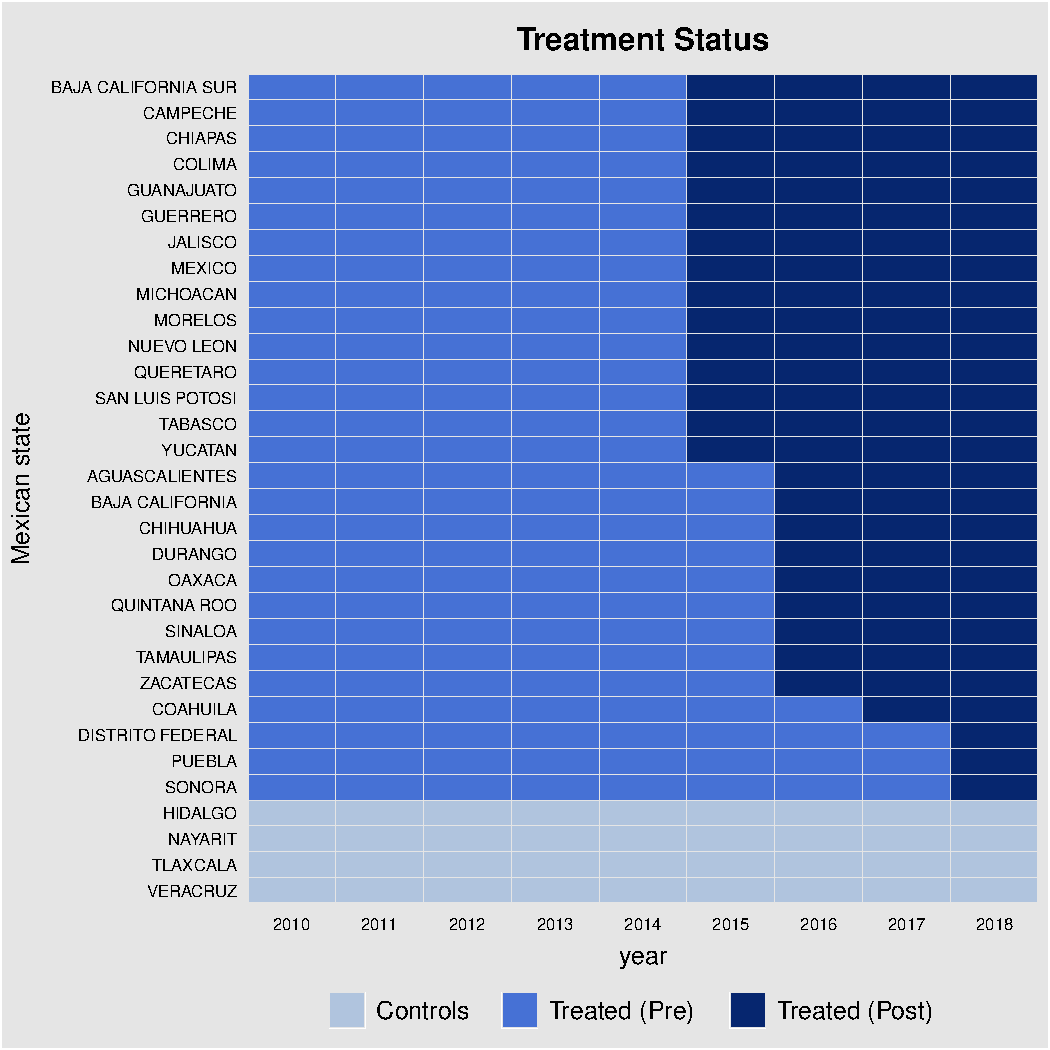
\includegraphics[width=0.75\textwidth]{Figures/reform_treatmentstatus.pdf}     
\captionsetup{justification=centering} 
\end{figure}   

 
A second source of discretion granted to state-level legislatures revolved around the reelection implementation date. The reform dictated that any change would not affect 2014 elections, and would be implemented for federal legislators till the elections of 2018. For local legislators and mayors, however, state-legislators defined the implementation period. Given governors influence in candidate selection of legislators (and mayors in some cases), their staggered calendar and political power seems to explain most of the variation in the timing of the implementation of the reform: governors with terms ending near the Reform approval date (2014) introduced reelection as early as possible, while those whose terms where starting pushed reelection further down the line \citep{motolinia_2020}.\footnote{For more detail on the political background of the Electoral Reform see Appendix \ref{appendix:reform_backgorund}.}
   
Figure \ref{fig:treatment_status} describes the implementation period or treatment status of each of Mexico's 32 states.\footnote{Mexican states share the same administrative level as US states.} This figures allows to visualize the staggered rollout of the term limit removal. We have five timing groups. Four states never receive treatment during this time period (Hidalgo, Nayarit, Tlaxcala and Veracruz), while the rest commence treatment in different years from 2015 to 2019. %The always-treated group is composed by the states of Baja California Sur, Campeche, Chiapas, Colima, Guanajuato, Guerrero, Jalisco, Mexico, Michoacan, Morelos, Nuevo Leon, Queretaro, San Luis Potosi, Tabasco and Yucatan. 
    

\section{Data \label{sec:data}}  

I construct a novel database on security cooperation agreements signed by mayors with upper-level governments in Mexico from 2010 to 2018. I use the Municipal Government Census (\emph{Censos de Gobierno Municipal}) from 2011 to 2019 which collect information on the security capacity of municipalities, as well as their relationship with other governments and institutions. From 2011 to 2019 the census asked whether a municipality signed a centralized command agreement with the governor. From 2014 onwards it included additional questions of whether a mayor delegated security policy through a security cooperation agreement with other political actors including the President, governors from other states, mayors from other municipalities in the same state or other, as well as the conditions of agreements. I construct a dummy measure for whether a municipality had an agreement with the governor or not; likewise, I construct a dummy of whether they had an agreement with other political actors. I construct dummy variables for the conditions of agreements of whether the mayor decided to delegate public security activities, traffic, security prevention, training, sharing of equipment and technology, research capacity, analysis and intelligence and the formation of unified criteria on procedures of public security institutions and laws. I also construct dummy variables on the reasons expressed to signing the security cooperation agreement with the governor, including a constitutional reform, change in local legislation, lack of resources, need of professionalization, a need for coordination, and given the prevalence of crime.
 

To proxy for citizens security preferences, I rely on the National Survey of Victimization from 2011 to 2019 (\emph{ENVIPE} in Spanish). ENVIPE collects state-level representative data on the year previous to the collection.  In particular, I focus on the question of the topic that worries citizens the most which include any of the following: narcotraffic, insecurity, the punishment of criminals, corruption, poverty, unemployment, health, inflation, natural disasters, water scarcity and education. I construct the average rate of responses by state-year of these dummy variables. Four additional variables are constructed using the average response to the questions on the level of trust in police forces, whether citizens can identify them, their perceived level of corruption and efficiency.\footnote{The questions of trust and efficiency have a 4 item scale from ``a lot", ``somewhat", ``little", to  ``nothing" for either municipal, state or federal forces. I construct a dummy variable that takes the value of 1 for the items ``a lot" or ``somewhat" and 0 otherwise. The questions on whether citizens can identify each police force and corruption have only ``yes'' and ``no'' as response items. There are multiple police forces identified. I categorize them in the following way: traffic and preventive police forces correspond to the municipal level; state police and state attorney police forces to the state level; federal police, ministerial police, army and marines to the federal level.} 
 
Electoral data for recent Mexican elections at the governor and municipal level as well as data on the rollout of the electoral reform at the municipal level comes from \citet{magar_2012} and \citet{magar_2017}. The data compiled from multiple sources including state electoral institutes, Banamex Electoral Database, Voz y Voto, etc. contains voting counts per party as well as candidate lists at the governor level. I construct winning margins at the municipal and state level as the difference between the first and second runner.  Indicators to measure party-alignment between the federal executive, state and municipal governors are also build. These variables are used for controls. 

Lastly, to test the effect of the Term Limit Reform on public security and violence, I build a database on violence and effort placed by federal and municipal-level security forces for all municipalities in Mexico from 2010 to 2018.\footnote{Mexico has 2,467 municipalities. Thus, the total possible number of observation is 22,203 municipality-years (2,467 municipalities X 9 years).} The main outcome of interest is violence proxied by homicide related deaths collected by the National Institute of Statistics and Geography (INEGI for its acronym in Spanish).\footnote{INEGI reports two homicide datasets. One the one hand, homicide related deaths that come from the total death certificates marked as ``presumed homicides''. On the other hand, homicide statistics made up of the number of previous investigations initiated for the crime of homicide, by year and state. As noted by \citet{rivera_2012} these datasets do not coincide for a simple reason: the former counts bodies, the latter counts cases. I choose homicides based on death certificates since those based on initiated investigations tend to miscalculate the total number of deaths. For instance, borrowing a practical example by \citet{rivera_2012}, consider a mass grave with charred human remains. A preliminary investigation will count the number of deaths, and this will become part of the homicide related deaths figure. However, the investigation will only file one case, regardless of the number of victims found. I thus prefer to count victims rather than cases.} I measure homicides per capita to rule out municipality population differences. Population estimates come from the 2010 Census, the 2015 Population Count (both by INEGI), and CONAPO's population projections at the municipal level. Homicides per capita are highly skewed, with a long right tail of municipalities with substantially greater homicides than others. I therefore run the estimation on the impact of the reform on homicides per capita on logged values. For robustness, following \citet{mackinnon_maggie_1990}, I use the inverse hyperbolic sine (IHS) to transform the main outcome. %For robustness, I run estimates based on a second homicide database build by the SNSP.\footnote{For more detail on the SNSP homicide database please see Appendix \ref{appendix:SNSP_homicides}.}


To approximate the level of effort placed by municipal forces and the military I build a novel database on narcotics, arms and laboratories eradicated by the military -army and marines- from 2006 to 2019 at the municipal level  based on information petitions through the Mexican portal INFOMEX.\footnote{Information petitions number 0000700274419 and 0000700274519.} The dataset includes narcotic eradication (kg) of marijuana, heroine, methamphetamine, and cocaine, as well as marijuana and poppy kg per hectare erradicated, eradicated laboratories, and secured cartridges, vehicles, planes, short and long weapons as well as the detection of clandestine airstrips. %I aggregate the data to the yearly level by municipality. 
Another information petition to INFOMEX was made for municipalities to report the number of criminal detentions made month by month to proxy local level police effort. Detentions were aggregated at the yearly and municipal level. As with homicides, detentions and narcotic eradication and laboratories detected are highly skewed. I transform detentions to per capita logged values (also IHS), and narcotic and laboratories using logged (IHS) values as well. Lastly, to measure criminal presence, I rely on the 2010 cartel presence index from \citet{camilo_etal_2018}. 
 Appendix Table \ref{tab:descriptive} presents descriptive statistics of the variables used in the paper.

\section{Research Design \label{sec:design}}  

To investigate whether reelection incentives affected the delegation of security policy in Mexico, I explore the variation in the reelection incentives generated by the removal of term limits. This comparison has been widely used in the social sciences to identify the effect of reelection incentives (e.g., \citet{Besley_case_1995}; and see \citet{ashworth_2012} for a summary of its use in the literature). Specifically, I exploit the staggered implementation of the 2014 Electoral Reform in Mexico that removed term limits for local executives up to two periods. I compare first-term mayors who are term limited to first-term mayors who can be reelected, ``and so faced the same selection pressures, but have different incentives to impress the voters. Comparing these [incumbents] isolates the incentive effect.'' (\citet{ashworth_2012}, p.196). Comparing first term incumbents allows me to tease important endogenous concerns, particularly those arising from selection including differences in the experience and ability of incumbents \citep{ferraz_finan_2011}. 
   
%A first-term governor who can be reelected and a first-term governor who is term-limited have each won election once, and so faced the same selection pressures, but have different incentives to impress the voters. Comparing these governors isolates the incentive effect. A term-limited governor who has won election once and a term-limited governor who has won election twice both face the same incentives, but with different histories of selection. Comparing them isolates the electoral selection effect. Ashworth 2012.  

 To account for potential cohort treatment heterogeneity, I estimate  a cohort weighted event-study design following \citet{abraham_sun_2020} that exploits the staggered implementation of the reform and state-level variation.\footnote{A two-way fixed effect model at the municipal and year level would be the go to specification. However, recent literature has shown that in the presence of staggered treatment timing and heterogeneous treatment effects across cohorts, the coefficient from two-way fixed effects models are not causally interpretable \citep{goodman_bacon_2018, callaway_santana_2019, strezhnev_2018, chaisemarting_etal_2019}. Furthermore, for event-study designs \citet{abraham_sun_2020} find that even under strong parallel trends assumption, pre-reform coefficients may not be non-zero and the post-reform coefficients may not correspond with a convex weighted averages of cohort-specific treatment effects at particular lags and leads. In other words, coefficients of a given lag or lead can be biased by the effects from other time periods, and pretrends may be driven by treatment effect heterogeneity.}  
 I saturate the time and unit fixed effects structure so that treated units do not enter the test window as control units. Specifically, I replace the binary indicator variable for the start of the treatment reform with a series of lead/lag indicators $\gamma_k$ for being ``k" years away from treatment. I focus on the window from 8 years prior to treatment to three years afterwards i.e. for $k \in \{-8,3\} $ which correspond to the time period of 2010 to 2018, with 2015 the first year of Term Limit Reform implementation.\footnote{See Figure \ref{fig:treatment_status} where those treated in 2018 have 8 lags prior to treatment, while those treated in 2015 have 3 leads, the full window of analysis for $k \in \{-8,3\} $.} %In addition to including $\gamma_k$ for $k \in \{-8,3\} $, I saturate the model with indicators for years less than 3 years before treatment, and more than three years after treatment. 
I exclude the indicator on $\gamma_{-1}$ to avoid collinearity and for comparison: estimated coefficients are interpreted as the difference relative to $t-1$, i.e. one year prior to the implementation of the electoral reform. Following   \citet{abraham_sun_2020}, I also exclude $k=-8$ due to collinearity. The estimated equation is as follows:


 
 \begin{equation}
\label{eq:abraham} 
y_{mt}=\mu_m + \mu_t + \sum^{5}_{e=1} \sum^3_{k=-7, \neq {-8,-1}} \gamma_{e,k}(1\{E_i=e\} \cdot R^k_{m,t}) + \sum^{5}_{e=1} \sum^3_{k=-7, \neq {-8,-1}}  \Theta'X_{s(m)t} (1\{E_i=e\} \cdot R^k_{m,t}) + \epsilon_{mt}
%y_{mt}=\mu_m + \mu_t + \sum^5_{e=1} \sum^{3}_{k \neq {-8,-1}} \gamma_{e,k}(1\{E_i=e\} \cdot R^k_{m,t}) + \sum^5_{e=1} \sum^{3}_{k \neq {-8,-1}}  \Theta'X_{m(s)t} (1\{E_i=e\} \cdot R^k_{m,t}) + \epsilon_{mt}
%y_{mt}=\mu_m + \mu_t + \sum^5_{e=1} \sum^{3}_{k \neq {-1,-8}} \gamma_{e,k}(1\{E_i=e\} \mathbbm{1} (t-I_{m}=k)  ) + \sum\limits^{3}_{k=-8, k \neq -1} \Theta'X_{it} \mathbbm{1}(t-I_{m}=k) + \epsilon_{mt}
%y_{mt}=\mu_i + \mu_t + \sum^5_{e=1} \sum^{3}_{k \neq {-1,-8}} \gamma_{e,k}(1\{E_i=e\}\cdot R^k_{m,t} ) + \sum\limits^{3}_{k=-8, k \neq -1} \Theta'X_{it} \mathbbm{1}(t-I_{m}=k) + \epsilon_{mt}
\end{equation} 
  
where $y_{mt}$ is a dummy that takes the value of 1 if a municipality has a cooperation agreement with the governor, 0 otherwise. $E_i$ are cohort-specific indicators if a Mexican state removed term limits in a given year.\footnote{As noted in Figure \ref{fig:treatment_status}, there are five treatment cohorts including the never treated. The never-treated cohort is made up of the municipalities in the states of Hidalgo, Nayarit, Tlaxcala and Veracruz.} $R^k_{m,t}\in \{0,1\}$  is the Term Limit Reform treatment status indicator at period $k$ relative to treatment, for municipality $m$ at calendar time $t$.\footnote{$t=e+k$.} $X_{s(m)t}$ is a matrix of state $s$ (municipal $m$) level covariates interacted with the set of cohort-specific fixed effects including pre-treatment governor's winning margin, party alignment with the governor, party alignment with the President, mayor's winning margin, logged homicide related deaths per capita, and a dummy indicator on the presence of cartels.  The year indicators by treatment cohort  $\gamma_{e,k}$ are the difference-in-difference (DiD) estimators for the Cohort Average Treatment Effects (CATTs). Conditional on municipal and period fixed effects, as well state-level covariates, these CATTs represent the annual difference in mean security agreements signed with governors between municipalities that removed term-limits relative to those that did not, $k$ years before and after treatment. Standard errors are clustered at the state-level as that is the treatment level of the Term Limit Reform. Since the number of clusters is small (32 states), I adjust standard errors using wild bootstrap when indicated. 

I take the linear combination of the CATTs for each relative time period $k$, weighting each cohort by its relative share of the sample, to construct the interaction weighted (IW) estimator of \citet{abraham_sun_2020}:   

\begin{equation}
\hat{\nu}_g=\frac{1}{|g|}\sum_{k \in g}\sum_e \hat{\gamma_{e,k}} \hat{Pr}\{E_i=e | E_i \in [-k, T-k]\}	
\end{equation}

where $\hat{\gamma_{e,k}}$ is returned from equation \ref{eq:abraham} and $\hat{Pr}\{E_i=e | E_i \in [-k, T-k]\}$  are the estimated weights equal to the share of each cohort in the relevant time period, normalized by the size of  $g$, with $g$ the universe of the $k$ periods relative to treatment. Since I estimate a IW estimator per year $|g|=1$. Lastly, to estimate the average treatment effect from $t$ to $t+3$ I run the linear average of weighted coefficients across the CATTs of those time periods relative to treatment. 

\section{Main Results \label{sec:results}}


   
Figure \ref{fig:event_study_agreements} reports the IW estimator %\footnote{From here on all tables report IW estimators.} 
 for each lead and lag relative to the first year a municipality implemented reelection. In average from $t$ to $t+3$ , reelection incentives decreased delegation of public security provision to the governor by 41.97\% significant to the 5\% level. In magnitude, this result represents 1.5 times the mean or almost 1 standard deviation. In other words, compared to term limit incumbents, incumbents seeking reelection will decrease the delegation of public security provision to the governor. This is true whether we adjust the standard errors for the small number of clusters using Wild bootstrap or not (see Appendix Table \ref{tab:as_agreements}).\footnote{Including a lag outcome may introduce Nickell bias. More importantly, the lagged outcome conflates controls for heterogeneity and modeling dynamic treatment effects. To avoid these problems I only control for pretreatment outcomes to deal with heterogeneity and do not include  any lags of the dependent variable. Alternatively, I use matching on pre-treatment outcomes and find that results show similar effects (see Section \ref{sec:robustness}).}   
         
     
If delegation of security policy decreases, what specific services are provided by incumbents? Figure \ref{fig:services} shows that incumbents with reelection incentives decrease signing agreements that delegate the service of public security (-10.31\% significant to the 1\% level) and also public traffic (2.4\% significant to the 5\% level). Meanwhile, those related to capacity building are not different relative to term-limited mayors including training, equipment and technology, research and intelligence and the unification of laws and procedures. 

\begin{figure}[h] 
\centering
 \caption{Effect of Term Limit Reform on Security Cooperation Agreements signed with the Governor, 2010-2018}
 \label{fig:event_study_agreements}
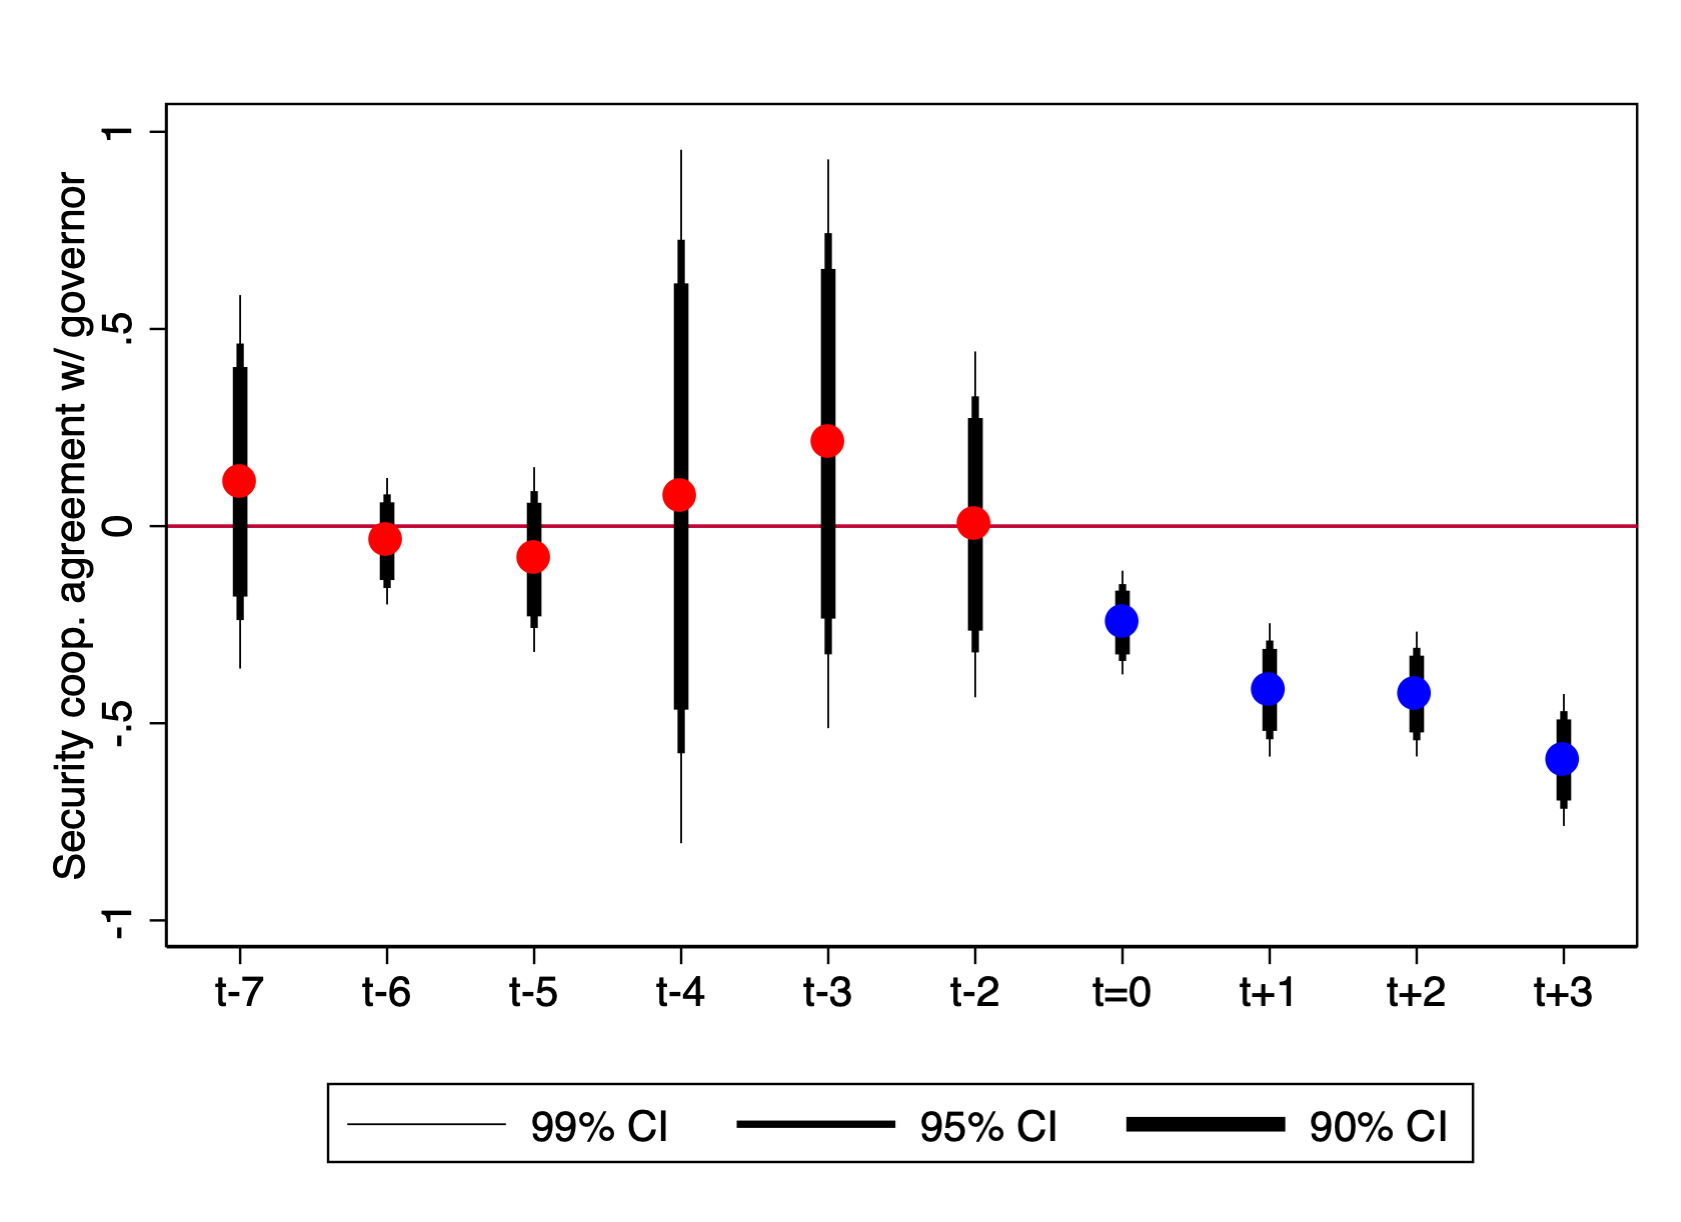
\includegraphics[width=0.75\textwidth]{Figures/catts_agreements.png}
       \captionsetup{justification=centering}
       
 \textbf{Note:} Figure \ref{fig:event_study_agreements} shows the IW estimators following \citet{abraham_sun_2020} for each lead and lag relative to the first year a municipality implemented reelection. Red points are pre-treatment, while blue ones post-treatment. 
     
\end{figure}   

 \begin{figure}[h]   
\centering
 \caption{Comparison: Security Cooperation Agreements with Governor vs. Other Actors, 2014-2018}
 \label{fig:services}
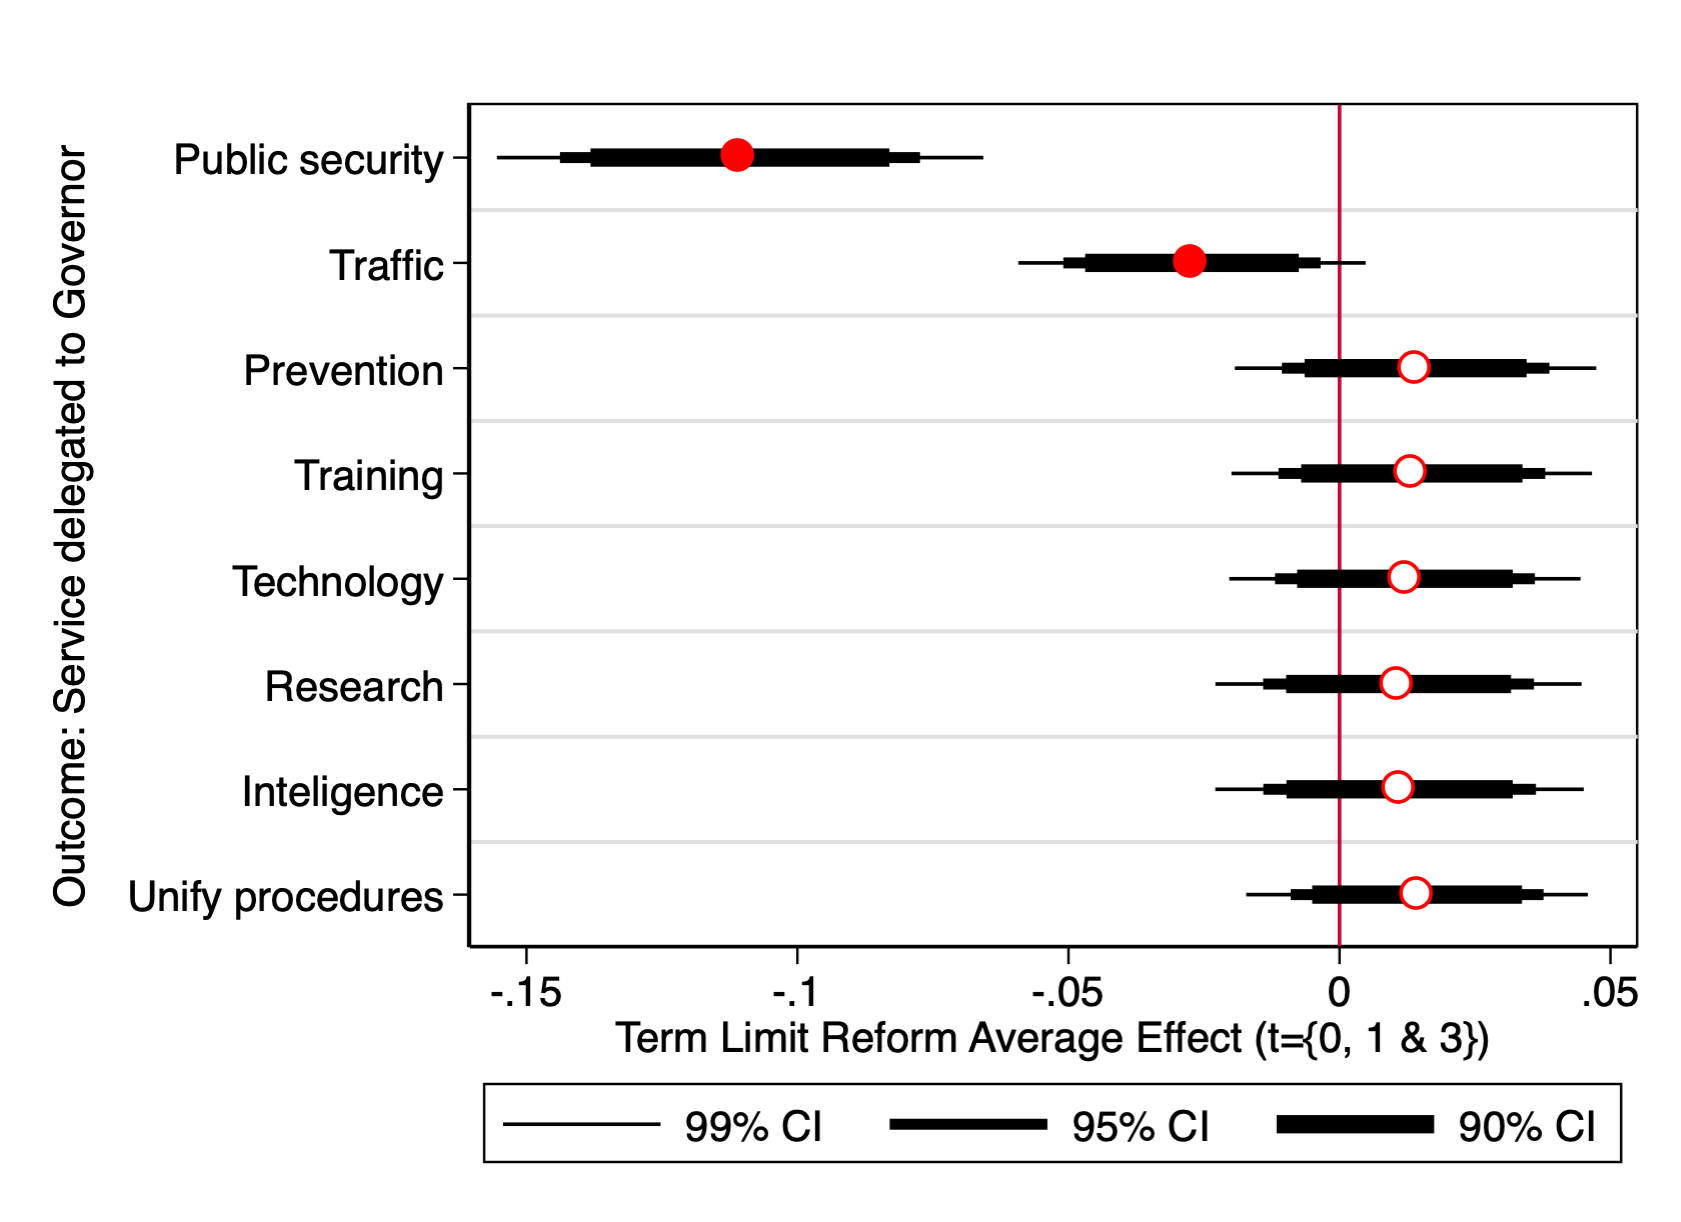
\includegraphics[width=0.65\textwidth]{Figures/services.png}
       \captionsetup{justification=centering}
       
 \textbf{Note:} Figure \ref{fig:services} shows the average treatment effect from t, t+1 and t+3 across multiple specifications. This average effect was estimated using the IW estimators following \citet{abraham_sun_2020} for each lead and lag relative to the first year a municipality implemented reelection. Red points show that parallel trends hold, while hollow ones imply pretrends. 
\end{figure}  

\subsection{Identification \label{sec:identification}}
 
Once we consider cohort weights, I find strong evidence of parallel trends as noted in Figure \ref{fig:event_study_agreements}. Besides no pretrends, identification in this setting implies that the staggered roll-out of the Term Limit Reform is orthogonal to municipal-specific characteristics, conditional on municipal and year fixed effects. This implies {\emph as-if} random assignment to the treatment status visualized in Figure \ref{fig:treatment_status}. If say, strong governors delay or adjust the implementation of the reform according to their political agenda or calendar, then identification would fail. To address this problem equation \ref{eq:abraham} interacts the state covariates with cohort-specific fixed effects to adjust for any changes correlated to the evolution of governors strength, the term $X_{s(m)t} (1\{E_i=e\} \cdot R^k_{m,t})$. Pretreatment covariates include governor winning margin and an indicator of governor party alignment with the Federal Executive, since pressure from former President Enrique Pena Nieto modified state legislators approval of the electoral reform, particularly for PRI states (for more detail see Section \ref{sec:reform}). Identification assumption implies now that conditional on municipal and year fixed effects, and cohort specific linear trends in state-level covariates, unobserved factors are not correlated with the electoral reform treatment assignment over time.\footnote{I further validate this by following \citet{altonji_etal_2005} to check if unobserved variation is likely to explain the signing of security cooperation agreements with the Governor by mayors. I regress the treatment (whether the municipality held reelection) on all the available covariates used for Figure \ref{fig:event_study_agreements}. I then take the fitted value from the regression and use it to predict each outcome, this time including unit and year fixed effects. Appendix Table \ref{tab:unobservables} suggests that – under the assumption that observables are representative of unobservables – selection on unobservables is not driving the results.}   

An additional identification assumption in event-study designs speaks to no anticipatory behavior from municipalities (or states) to the implementation of reelection. If states have private knowledge of the future treatment path this may change their behavior in anticipation to being treated and thus the potential outcome prior to treatment may not be that of baseline outcomes: estimated coefficients may reflect the anticipatory effects of the reform rather than differences in untreated potential outcomes between untreated and treated groups. %\citep{malani_rief_2015}.
%In this setting, knowledge from incumbents of the term limit removal could lead to a decrease in public security (and public good) provision since this will be the period a term limited politician could extract rents or pursue clientelistic practices without the electoral penalty of reelection. The violation of this identification assumption would lead to a (positive) bias of concern. 
I test this assumption by comparing if early and late adopters differed in their estimated effects. As seen in Appendix Figure \ref{fig:CDLZ_agreements}, this is not the case: there is wide variation in estimated coefficients across early (red) and late (blue) adopters of the reform.\footnote{For more detail on how I compare early to late adopters, please see Appendix \ref{appendix:CDLZ}.}  

In short, taking together parallel trends, evidence on no-anticipatory behavior from municipalities (and states) and cohort weighted estimates that account for treatment effect heterogeneity, I find a robust and unbiased negative effect of reelection incentives on the delegation of security policy.  The following section further probes the results through different robustness and falsification tests.
         

\section{Robustness \label{sec:robustness}}
 
  Figure \ref{fig:robustness_agreements} compares 6 models (see also Appendix Table \ref{tab:as_aggregate}). I find the naive two-way fixed effect model by municipality and year to reflect a negative non-signifiant effect. However, pretrends are found and results need to be interpreted with caution as non-weighted estimates are biased \citep{abraham_sun_2020}. Adjusting standard errors using Wild bootstrap yields similar results. However, the main model with and without standard error adjustment shows parallel trends and significant results. This result holds when changing the reference period from $t-1$ to $t=0$. Results also hold when performing the common practice of trimming relative time periods relative to treatment \citep{borusyak_2017, dobkin_etal_2018}, in this case by trimming all periods prior to $t-4$ to be balanced in relative periods. Moreover, across specifications the average effect from $t$ to $t+3$ remains relatively similar. %Overall, we see that the result that reelection incentives decreased delegation of security policy to the governor are robust across multiple specifications and models.
        
  
\begin{figure}[h]   
\centering
 \caption{Effect of Term Limit Reform on Security Cooperation Agreements signed with the Governor, 2010-2018}
 \label{fig:robustness_agreements}
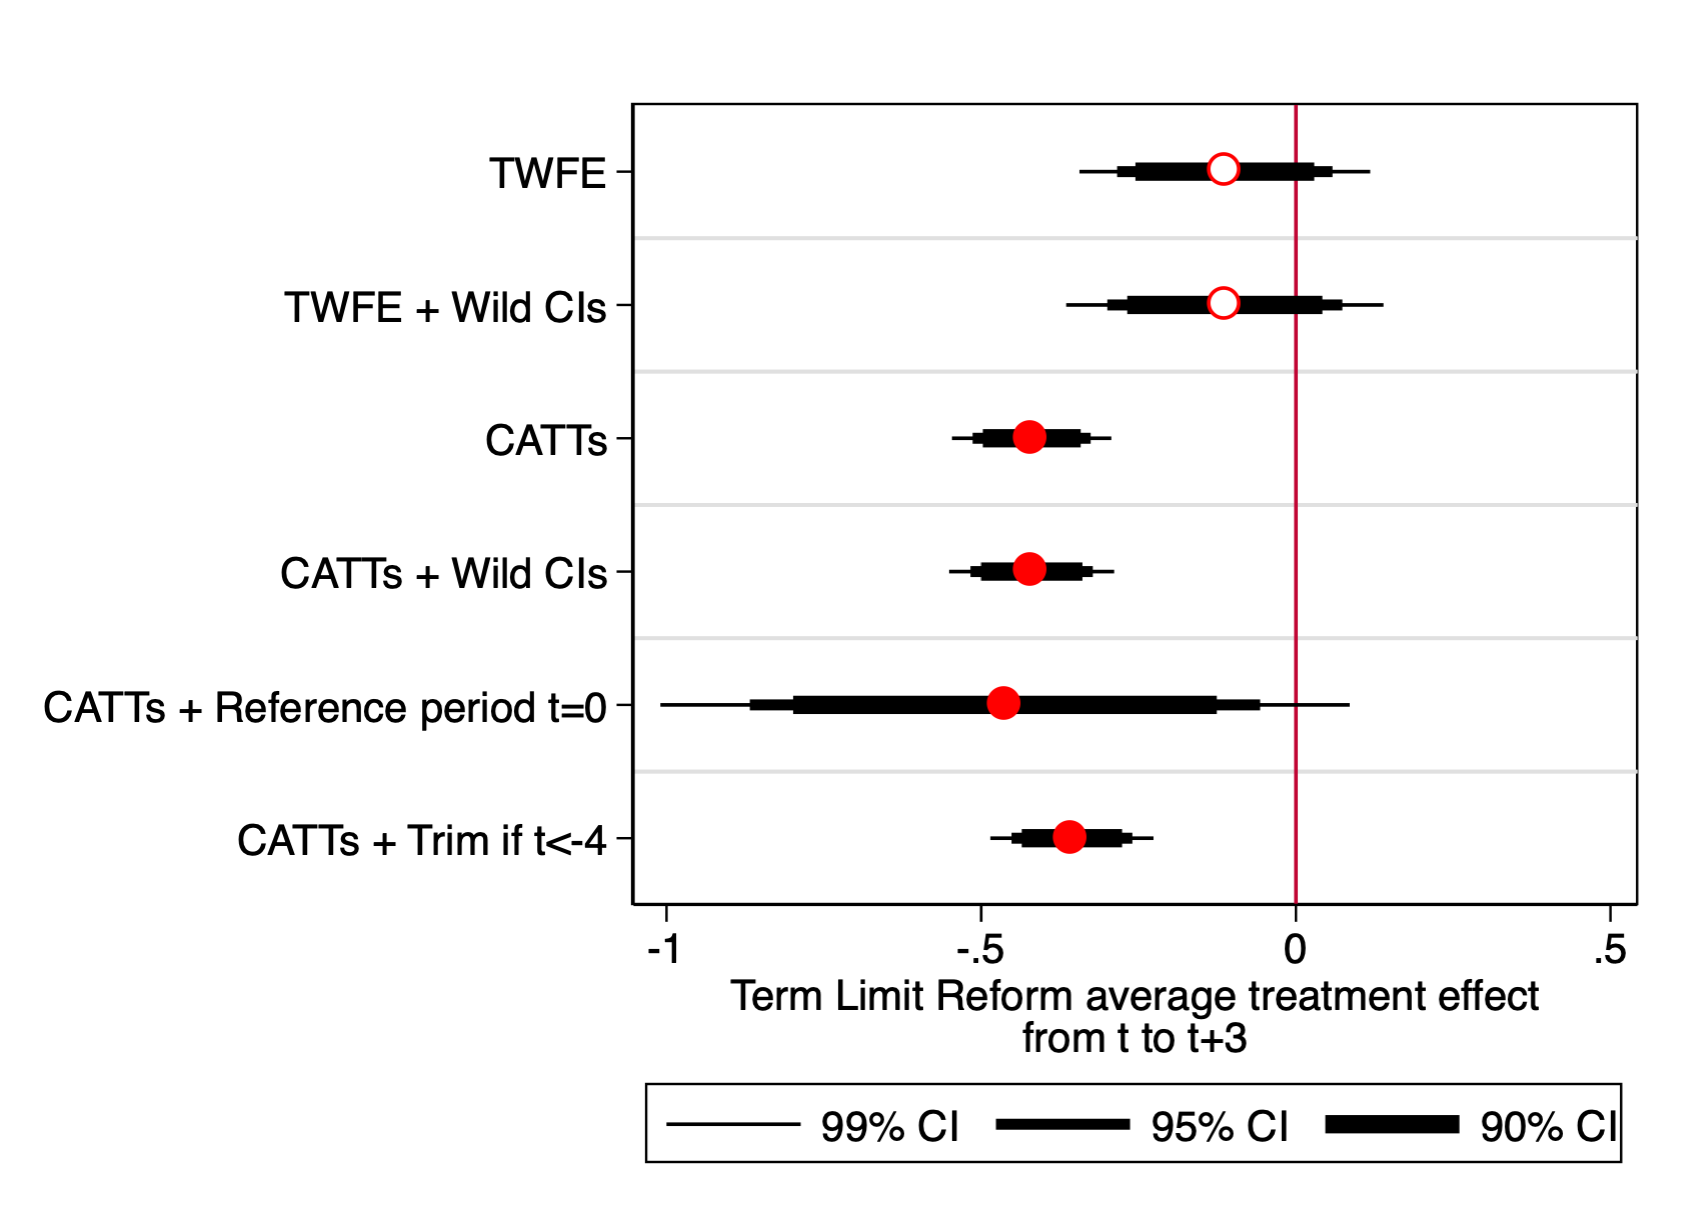
\includegraphics[width=0.75\textwidth]{Figures/average_effects.png}
       \captionsetup{justification=centering}
       
 \textbf{Note:} Figure \ref{fig:robustness_agreements} shows the average treatment effect from t to t+3 across multiple specifications. This average effect was estimated using the IW estimators following \citet{abraham_sun_2020} for each lead and lag relative to the first year a municipality implemented reelection. Red points show that parallel trends hold, while hollow ones imply pretrends. 
\end{figure}   

Now, I run a placebo test by seeing the effect of the reform on security cooperation agreements signed with actors like the President, and governors and mayors from other states. Local mayors have no interest in differentiating themselves from these actors and reelection incentives should not change the degree in which agreements are signed relative to local incumbents facing term limits. With governors, however, local mayors are in direct electoral competition. In Mexico, the federal structure creates a vertical competition between governors and local mayors primarily, i.e. when there are multiple public good service providers voters compare their efficiency and punish and reward them accordingly \citep{treisman_2000}.\footnote{The extent to which dual accountability exists varies by study case. See \citet{rodden_2010} for an example.} As a result, incumbents may over-provide public goods to differentiate themselves \citep{salmon_1987, Breton_1996, treisman_2000} and in this case decrease delegation. As expected,  the falsification test in Figure \ref{fig:comparison_fed_estatal} shows a positive and non-significant effect. 
    

 \begin{figure}[h]   
\centering
 \caption{Comparison: Security Cooperation Agreements with Governor vs. Other Actors, 2014-2018}
 \label{fig:comparison_fed_estatal}
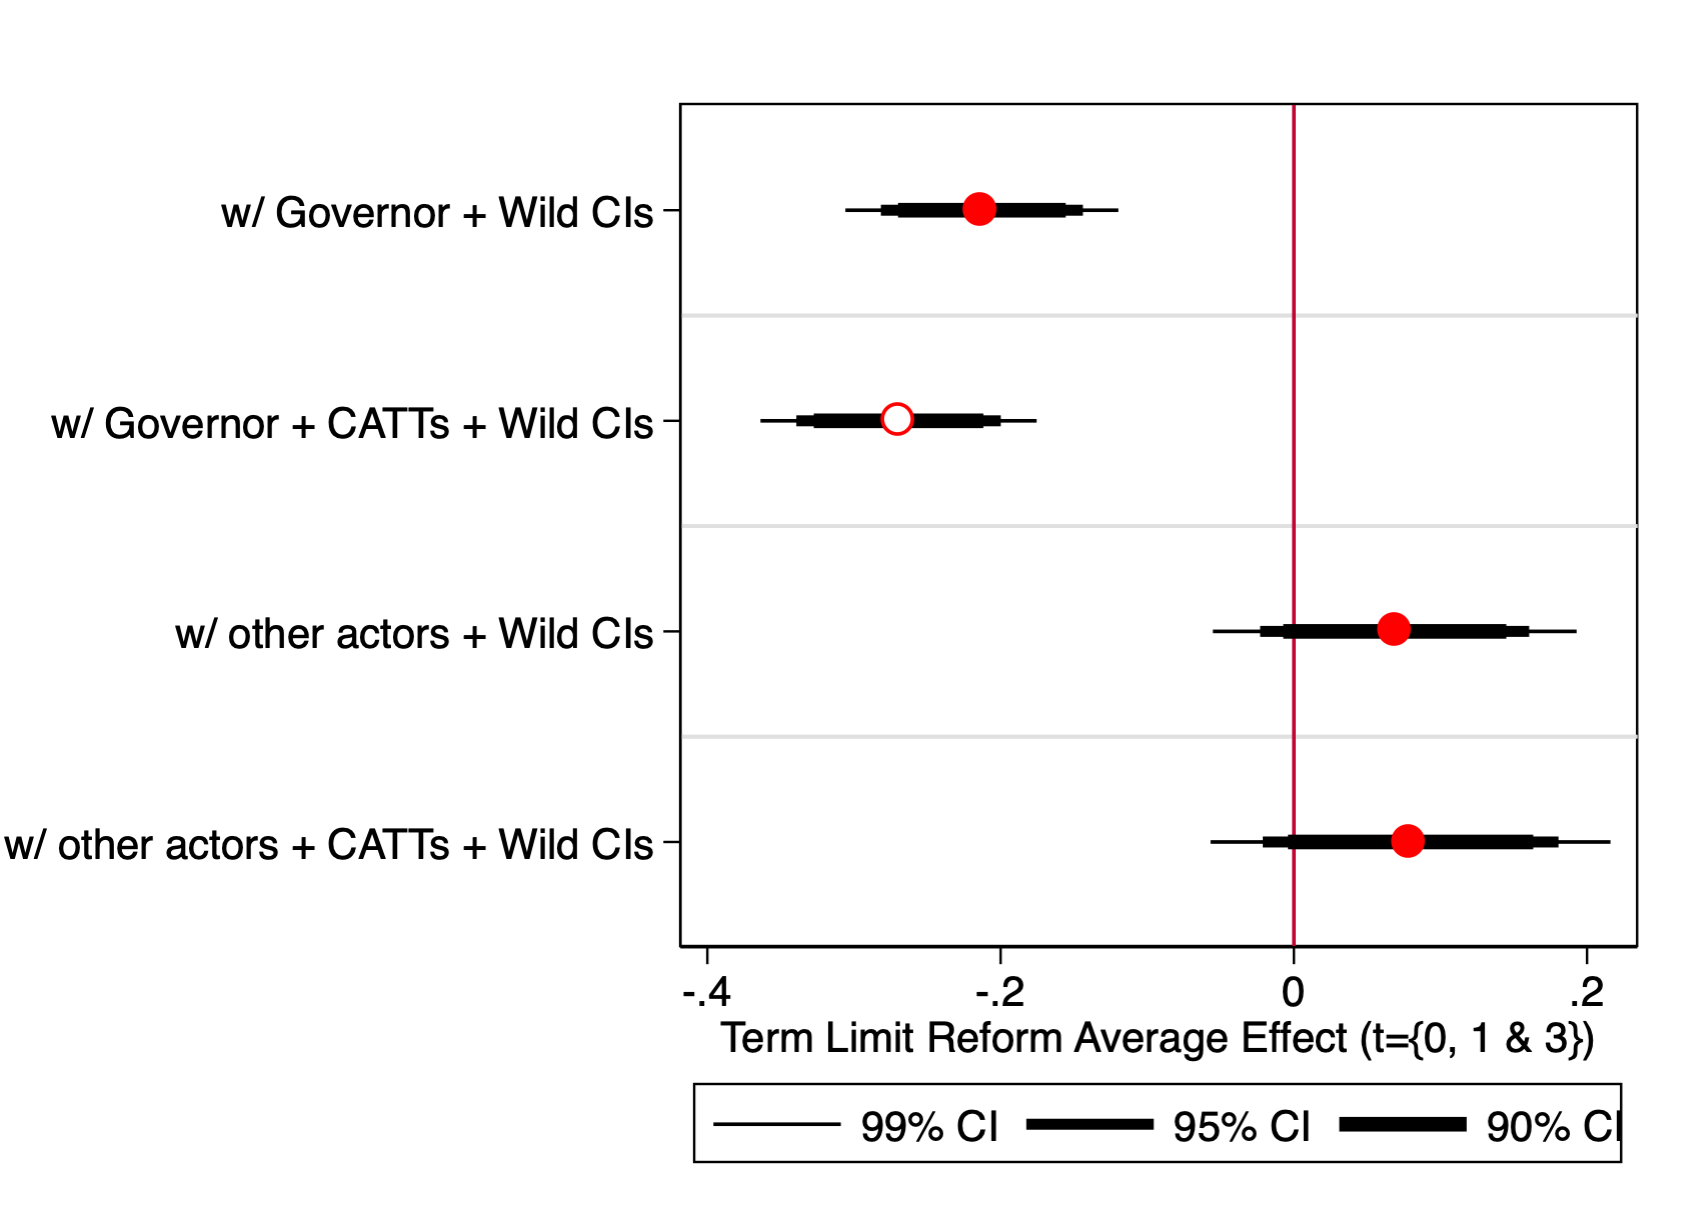
\includegraphics[width=0.75\textwidth]{Figures/average_effects_comparisonfedest.png}
       \captionsetup{justification=centering}
       
 \textbf{Note:} Figure \ref{fig:comparison_fed_estatal} shows the average treatment effect from t to t+3 across multiple specifications. This average effect was estimated using the IW estimators following \citet{abraham_sun_2020} for each lead and lag relative to the first year a municipality implemented reelection. Red points show that parallel trends hold, while hollow ones imply pretrends. 
\end{figure}   

Further validation is provided by the use of secondary research designs including \citet{imai_etal_2020} non-parametric generalization of the difference-in-difference estimator that does not rely on linearity assumption and corrects for invalid negative weighting in standard two-way fixed effects models (see Appendix Figure \ref{fig:matching}), as well as \citet{chaisemarting_etal_2019} difference-in-difference with multiple time period correction (see Appendix Figure \ref{fig:chaisemarting_agreements}).


\section{Mechanisms: Heterogeneous Effects by the Level of Concern of Narcotraffic by Citizens}

As discussed in Section \ref{sec:reelection_incentives}, we would expect incumbents with reelection incentives to be more responsive to policies that citizens deem as valuable \citep{milner_2004}. In such cases, electoral spoils are more efficient when the public good is more valuable to constituents \citep{lizzeri_2001}. In the context of American politics, for example, \citet{list_sturm_2006} find that governors seeking reelection adopt greener policies when their states hold large pro-environmental groups, while the opposite occurs in those with lower environmental support. In a similar tenor, we would expect that when citizens have high concerns for security policy then incumbents with reelection incentives will provide security directly. This is what we find in Figure \ref{fig:preferences_all} that runs an interaction between the treatment of the Electoral Reform on narcotraffic as the topic that citizens´ worry the most. When there is a low concern of narcotraffic the effect is statistically indistinguishable from zero. However, when citizens have high concerns of narcotraffic mayors racing reelection decrease the delegation of security policy to governors relative to term-limit mayors. This is particularly salient with narcotraffic, but not for overall insecurity or the desire of punishment to criminals. It is important to note that this finding is conditional on    pre-treatment violence levels, i.e. the differences in the concern of narcotraffic or delegation are not explained by differences in levels of violence but variation in idiosyncrasies between states of Mexico. As a  falsification test,  Figure \ref{fig:preferences_all} includes other topics that citizens worries the most but are not related with public security provision. Overall, we see null findings and in some cases they are even positive. These cases belong to topics that are ``too big'' or of the national order in which cooperation is needed such as natural disasters and water scarcity. 
 
\begin{figure}[H]   
\centering
 \caption{Interaction effects by citizens' preferences}
 \label{fig:preferences_all}
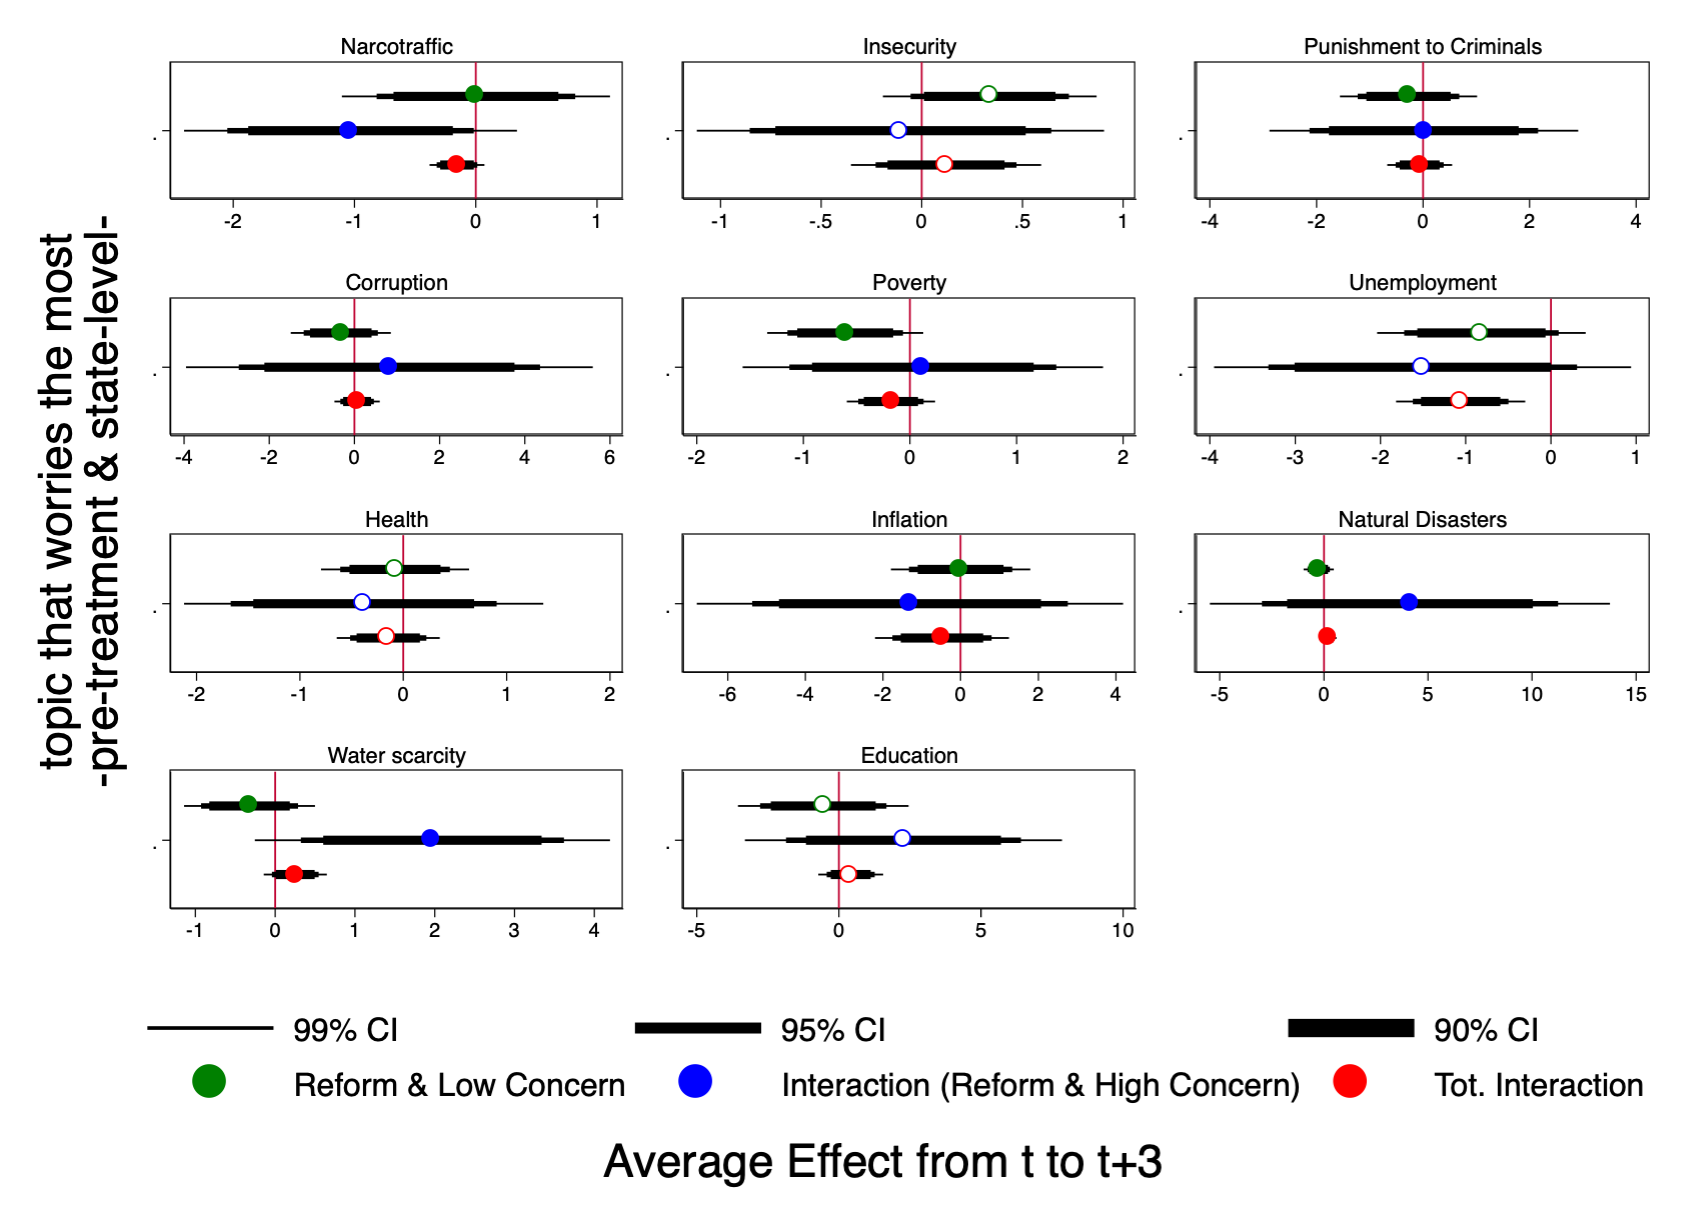
\includegraphics[width=1\textwidth]{Figures/preferences.png}
       \captionsetup{justification=centering}
       
 \textbf{Note:} Figure \ref{fig:preferences_all} shows the average treatment effect from t to t+3 across multiple specifications. This average effect was estimated using the IW estimators following \citet{abraham_sun_2020} for each lead and lag relative to the first year a municipality implemented reelection. Filled points show that parallel trends hold, while hollow ones imply pretrends.  
\end{figure} 
  
Now, political alignment is an important piece in the theory of responsiveness to citizens concerns: for incumbents with reelection incentives to care about citizens preferences, citizens need to be able to blame incumbents for public security inefficiencies. In the case of Mexico, \citet{ley_2017} shows that citizens hold the capacity to blame (and reward) local executives for inefficient (efficient) public security provision if their party is aligned with that of the governor. When not-aligned, citizens cannot clearly identify the responsible. This speaks to the claim that we should observe more delegation when the contributions of each level of government is clear to citizens \citep{treisman_2000}. Figure \ref{fig:alignment} shows the interaction effect of party alignment on the Term Limit Reform. As expected in the first panel, when there is alignment with the President the effect is statistically zero: citizens in this case are not capable to blame local incumbents for public security inefficiencies. However, when aligned with governors they hold such capacity, and as a response incumbents seeking reelection decrease the delegation of security policy to governors (second panel). This is particularly salient for those aligned both with PRI governors (third panel). Interestingly, a bigger negative point estimate exists for those not aligned, i.e for incumbents from an opposition party, but results are not statistically different from zero. 

In conclusion, compared to aligned and not aligned term limit incumbents, incumbents seeking reelection and aligned with the governor will decrease the delegation of public security provision to the governor. Moreover, there is no difference in this behavior when aligned with other political actors like the President where alignment does not make citizens capable of blaming or rewarding the responsiveness of incumbents in the issue of security policy. %we also see a more negative point estimate when incumbents are not aligned, that is when incumbents are from an opposition party. While there is no statistical difference with those who are aligned, the difference in point estimates goes in line with the prediction that political alignments across different levels of government jeopardize the implementation of national policies: when opposition parties control subnational levels of government, they hinder the implementation of national and regional policies creating a heterogeneity in terms of coverage. For example, \citet{niedzwiecki_2018} shows this to be the case for conditional cash transfer and health programs in Brazil and Argentina where non-alignment jeopardizes the implementation of national policies.

\begin{figure}[H]   
\centering
 \caption{Reform interaction with Party Alignment}
 \label{fig:alignment}
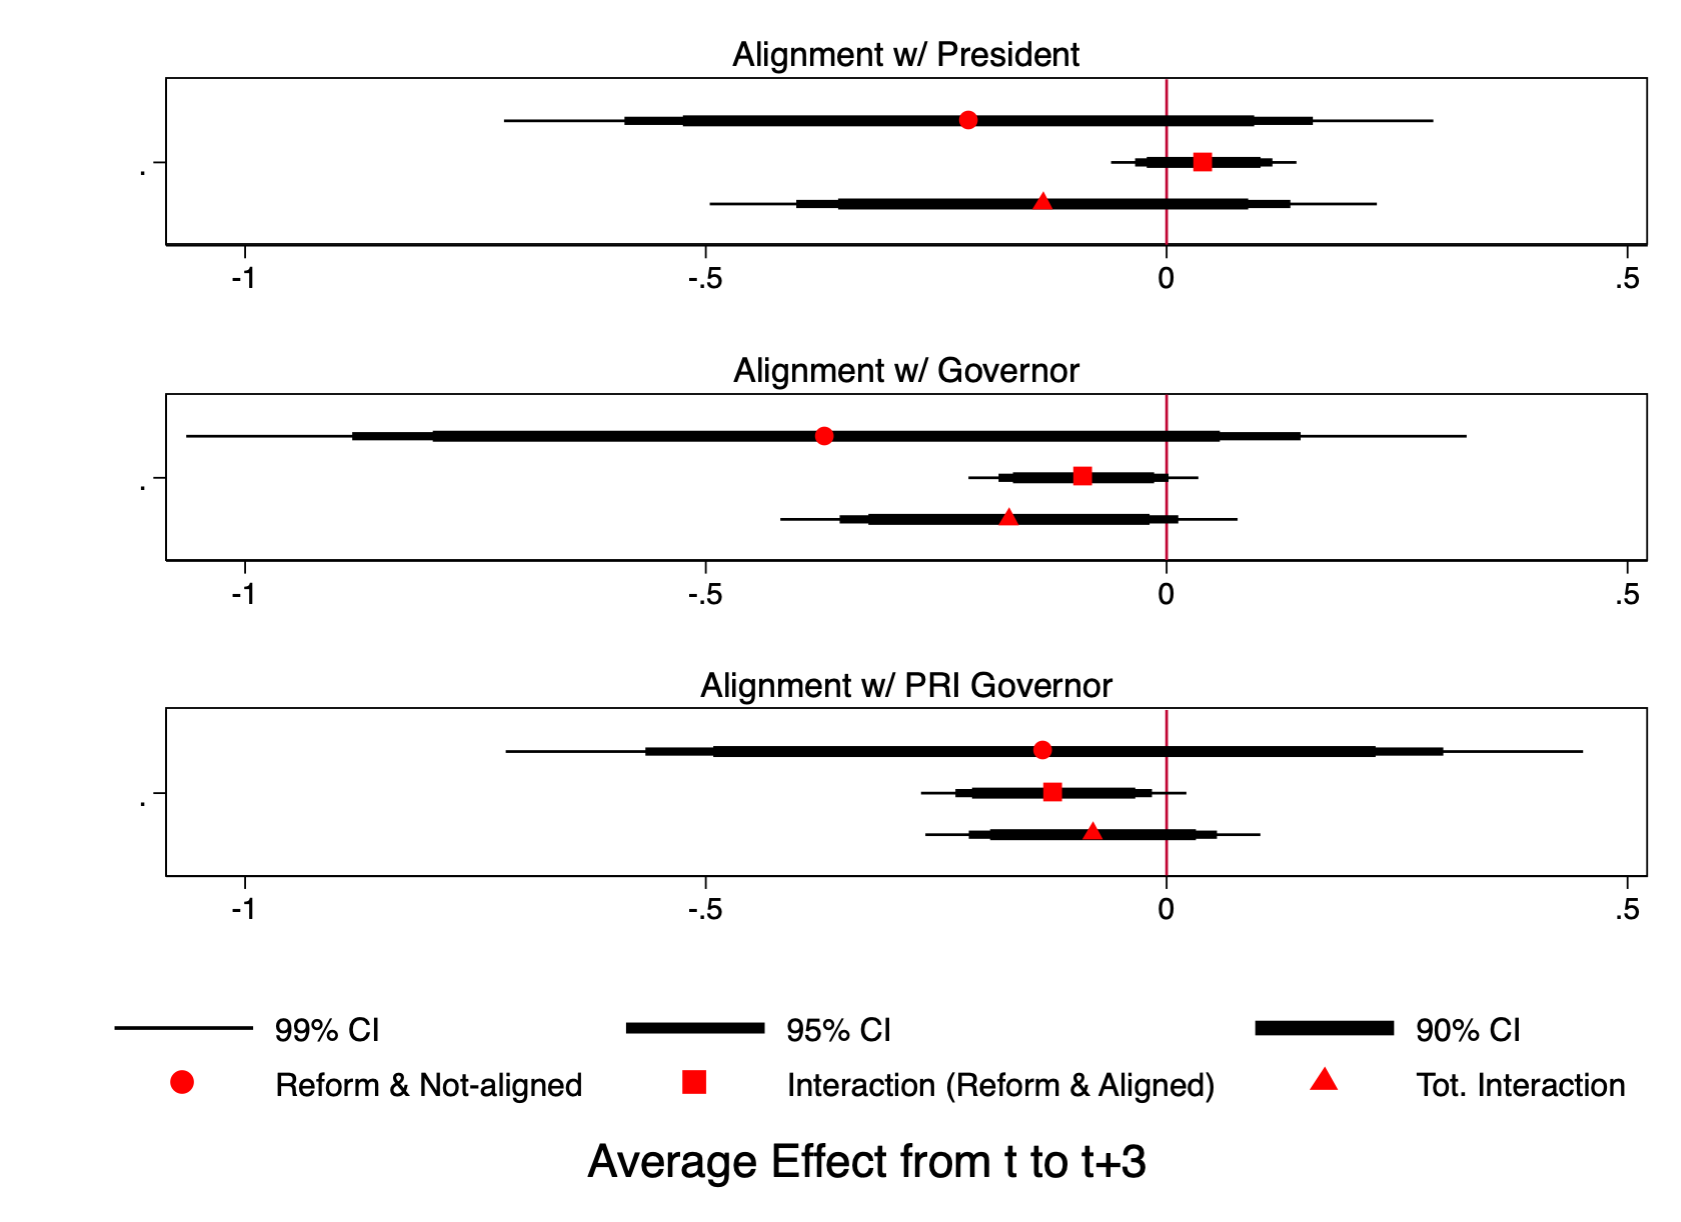
\includegraphics[width=0.9\textwidth]{Figures/interaction_alignment_full.png}
       \captionsetup{justification=centering}
       
 \textbf{Note:} Figure \ref{fig:alignment} shows the average treatment effect from t to t+3 across multiple specifications. This average effect was estimated using the IW estimators following \citet{abraham_sun_2020} for each lead and lag relative to the first year a municipality implemented reelection. Red points show that parallel trends hold, while hollow ones imply pretrends. To check parallel trends see Appendix Figure \ref{tab:interaction_alignment}.  
\end{figure}  
\begin{comment}
	
In a similar tenor, incumbents up for reelection should portray responsiveness by taking charge of security policy when police forces from upper-level jurisdictions are not deemed as reliable. The keft graph of Figure \ref{fig:trust_identify} shows the total interaction effect of the interaction of trust and the Term Limit Reform 

and the whether citizens are able to identify a police force on t

that delegation decreases when state and federal forces are not trusted 

4. Mayors facing reelection do not sign agreements when other security forces are highly trusted or identified.

\begin{figure}[H]   
\centering
 \caption{Total interaction effects by citizens' trust and identification of police forces}
 \label{fig:trust_identify}
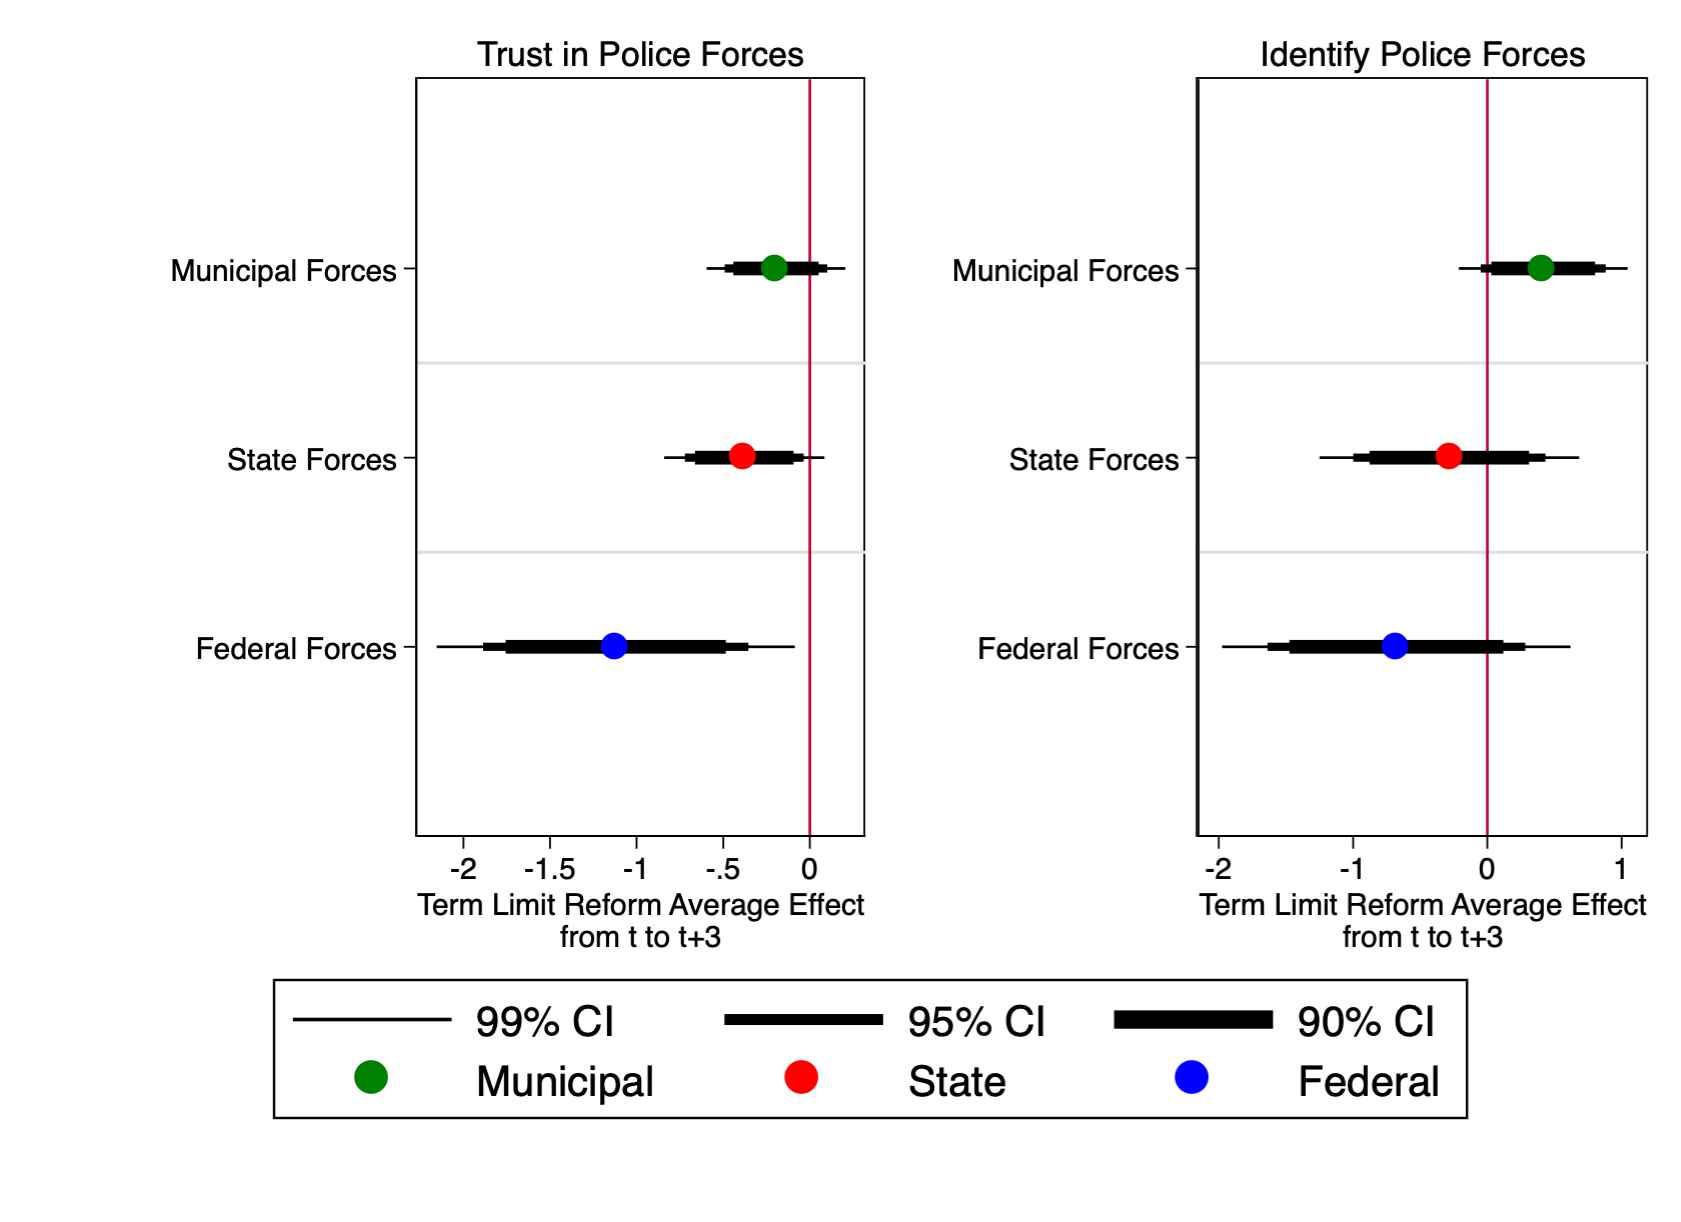
\includegraphics[width=1\textwidth]{Figures/trust&preferences.png}
       \captionsetup{justification=centering}
       
 \textbf{Note:} Figure \ref{fig:trust_identify} shows the average treatment effect from t to t+3 across multiple specifications. This average effect was estimated using the IW estimators following \citet{abraham_sun_2020} for each lead and lag relative to the first year a municipality implemented reelection. Filled points show that parallel trends hold, while hollow ones imply pretrends.       
\end{figure}   
   
  \end{comment}

\section{Ruling out Alternative Hypothesis: Cartel Presence and Captured Incumbents}

A reason why reelection may decrease delegation to upper-level governments is state capture. Public good provision entails, sometimes, the interaction with a third player. For example, incumbents interrelate with firms who compete for procurement bids. In the process, however, incumbents may be captured, changing the market structure and decreasing welfare. This is even more prevalent with longer tenures \citep{coviello_etal_2017}. As noted by  \citet{canen_etal_2020} influence groups are strategic and react to the uncertainty of the political environment by capturing the local apparatus. Incumbents may be captured by non-state armed groups who modify local institutions in favor of their self interest \citep{ch_etal_2018}, including a reduction in state-led violence agains them which could be achieved by not delegating security policy to more capable agents like the governor. 

Moreover, in the paper, so far, I have assumed that DTOs are non-strategic players. However, this assumption is hard to defend: incumbents with longer tenures are more likely to be captured by DTOs. In such case, we would expect a reduction in the delegation of public security. However, the research design only compares first term mayors with and without term limits. Moreover, all specifications and results control for the presence of cartels and homicide related deaths pre treatment. This rules out the possibility that findings are explained by capture and not reelection incentives.  

\begin{comment}
	
\subsection{Citizens' Evaluation of Corruption and Efficiency of Police Forces}

\begin{figure}[h]   
\centering
 \caption{Interaction effects by citizens' evaluation of efficiency and corruption of police forces}
 \label{fig:corruption}
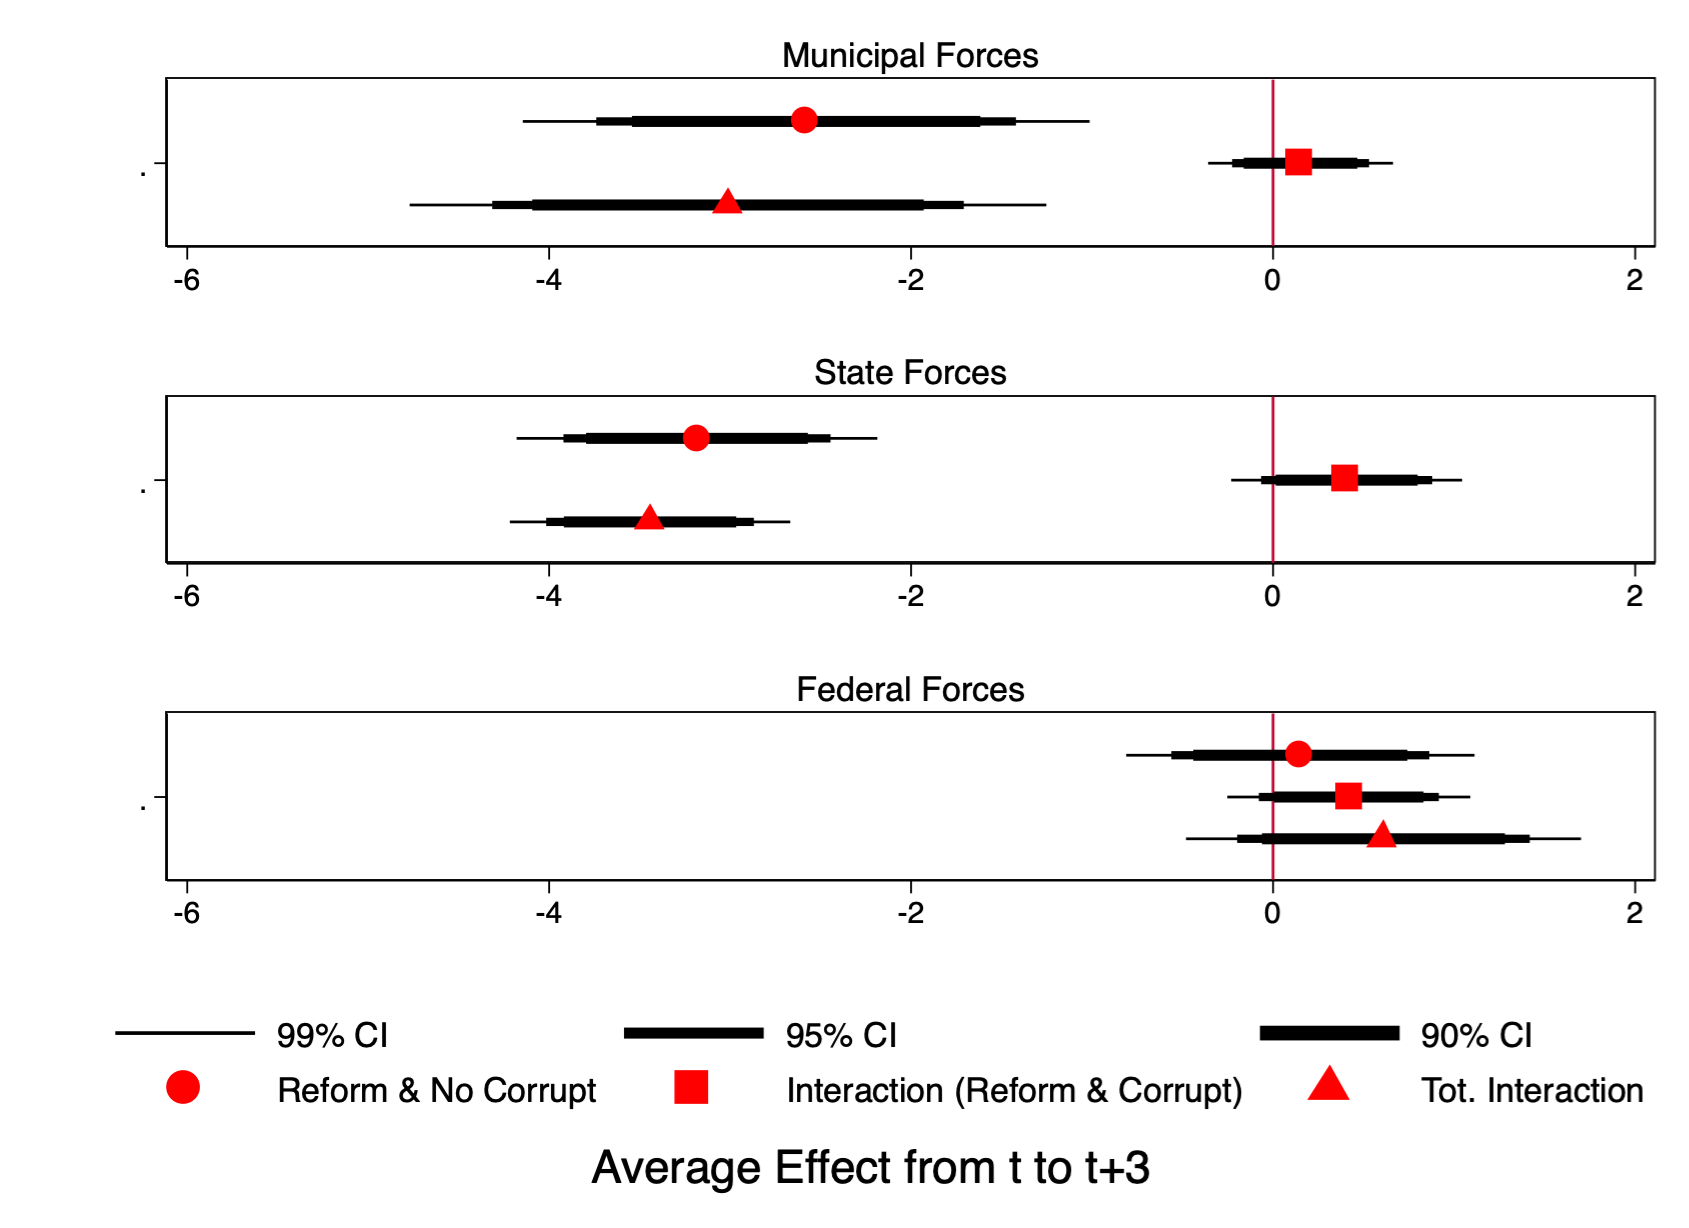
\includegraphics[width=0.7\textwidth]{Figures/corupt_byforces.png}
       \captionsetup{justification=centering}
         
 \textbf{Note:} Figure \ref{fig:efficiency_corruption} shows the average treatment effect from t to t+3 across multiple specifications. This average effect was estimated using the IW estimators following \citet{abraham_sun_2020} for each lead and lag relative to the first year a municipality implemented reelection. Filled points show that parallel trends hold, while hollow ones imply pretrends.        
\end{figure}   

Another potential concern that could confound the relationship between reelection incentives and the delegation of public security is corruption. Reelection incentives have been shown to decrease corruption \citep{ferraz_finan_2008, ferraz_finan_2011}, and delegations has been tied to a decrease in politicization and corruption \citep{Rodrick_1996}. While I cannot control for a measure of municipal corruption, we know that by comparing the first term of mayors with and without term limits we are avoiding the problems of selection, including experience and ability that could be correlated with corruption skills. A second exercise that can be done is the study heterogeneous treatment effects of the electoral reform on agreements by different levels of perceived corruption by citizens. Figure \ref{fig:corruption} show that when citizens see municipal state forces as not corrupt, 
\end{comment}

\section{Unintended consequences: Violence and Security Underprovision \label{sec:unintended}}
\begin{comment}
	
\subsection{Preferences for order and security}
1. PREFERENCES: citizens increase their valuation of insecurity as a pressing issue and decrease the valuation of other topics. Recall results are conditional on violence. So in the next election, they will vote for another hawk. This ties to the incumbency advantage.

\begin{figure}[H]    
\centering
 \caption{Effect of Term Limit Reform on Citizens' Preferences}
 \label{fig:preferences}
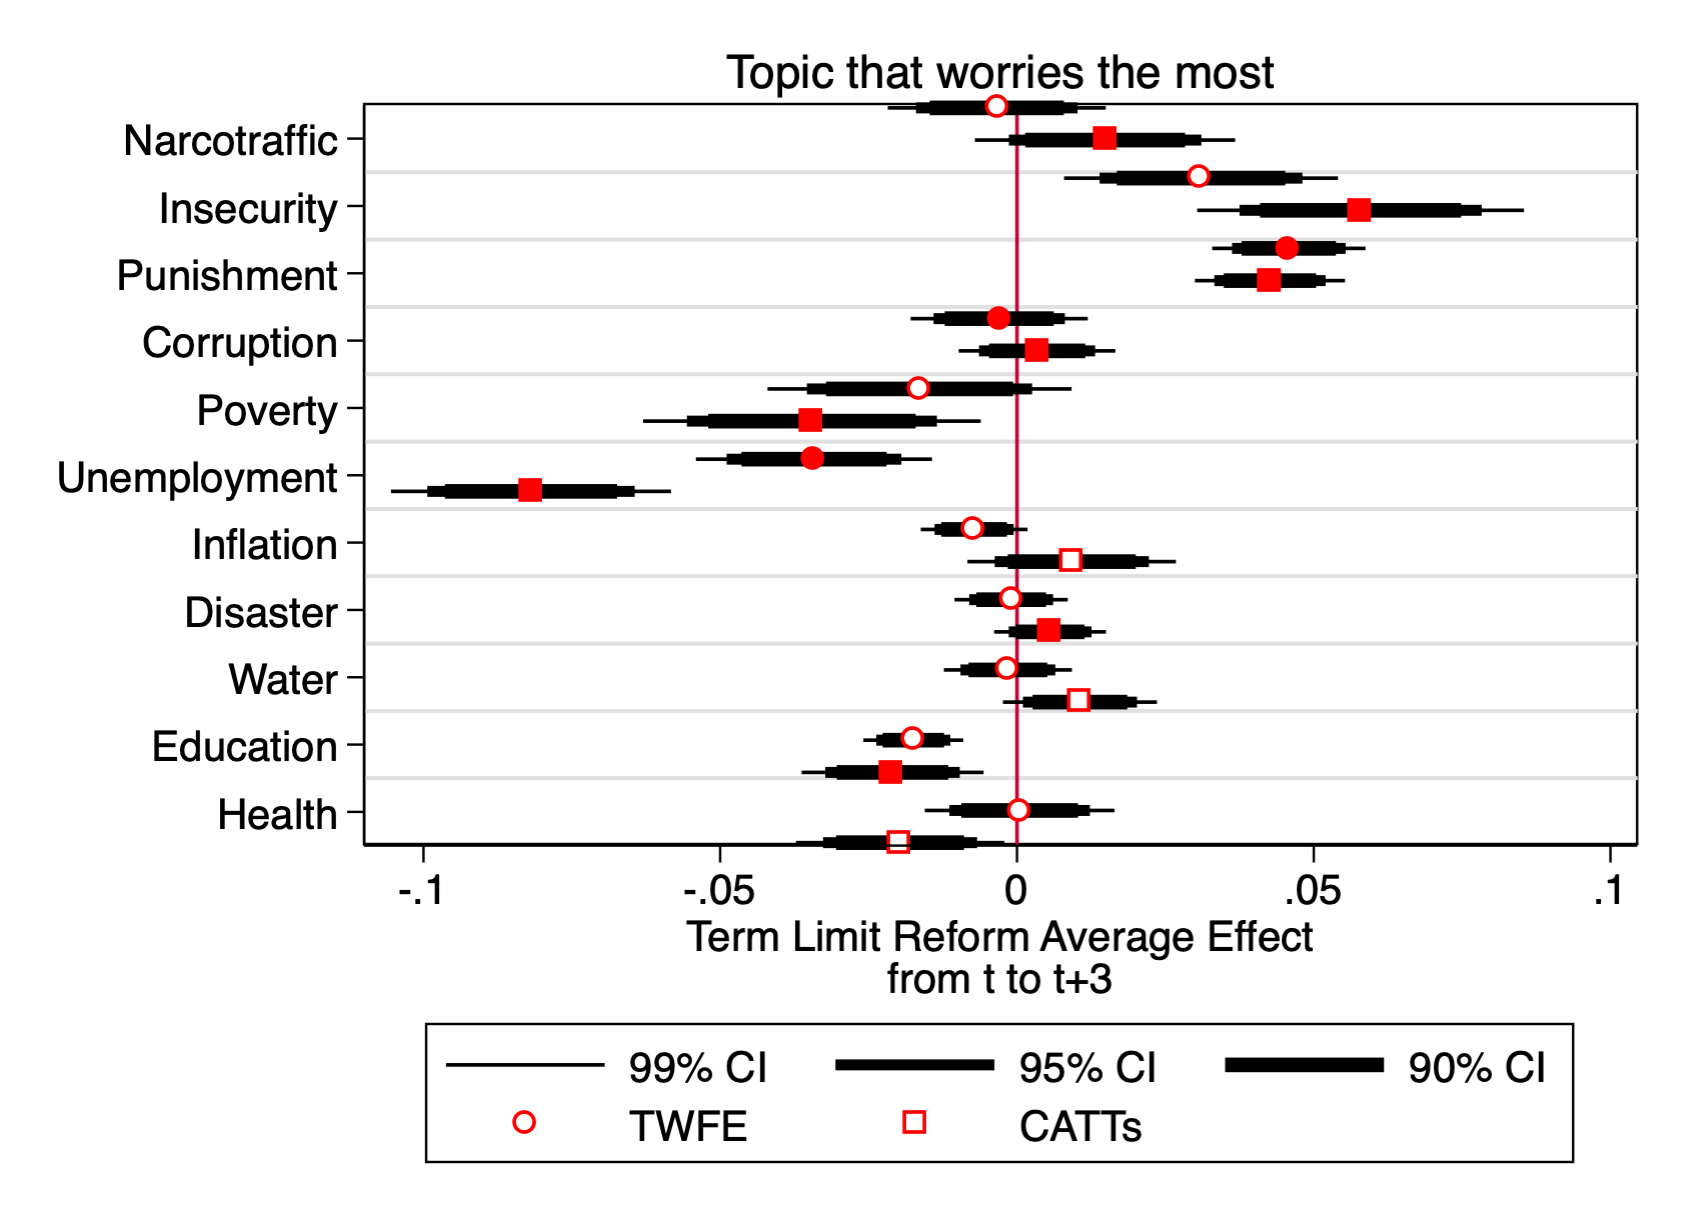
\includegraphics[width=1\textwidth]{Figures/change_preferences_comparison.png}
       \captionsetup{justification=centering}
         
 \textbf{Note:} Figure \ref{fig:preferences} shows the average treatment effect from t to t+3 across multiple specifications. This average effect was estimated using the IW estimators following \citet{abraham_sun_2020} for each lead and lag relative to the first year a municipality implemented reelection. Filled points (squares) show that parallel trends hold, while hollow ones imply pretrends.        
\end{figure}   
 
\end{comment}

\begin{figure}[h] 
\centering
 \caption{Effect of Term Limit Reform on Violence}
 \label{fig:as_violence}
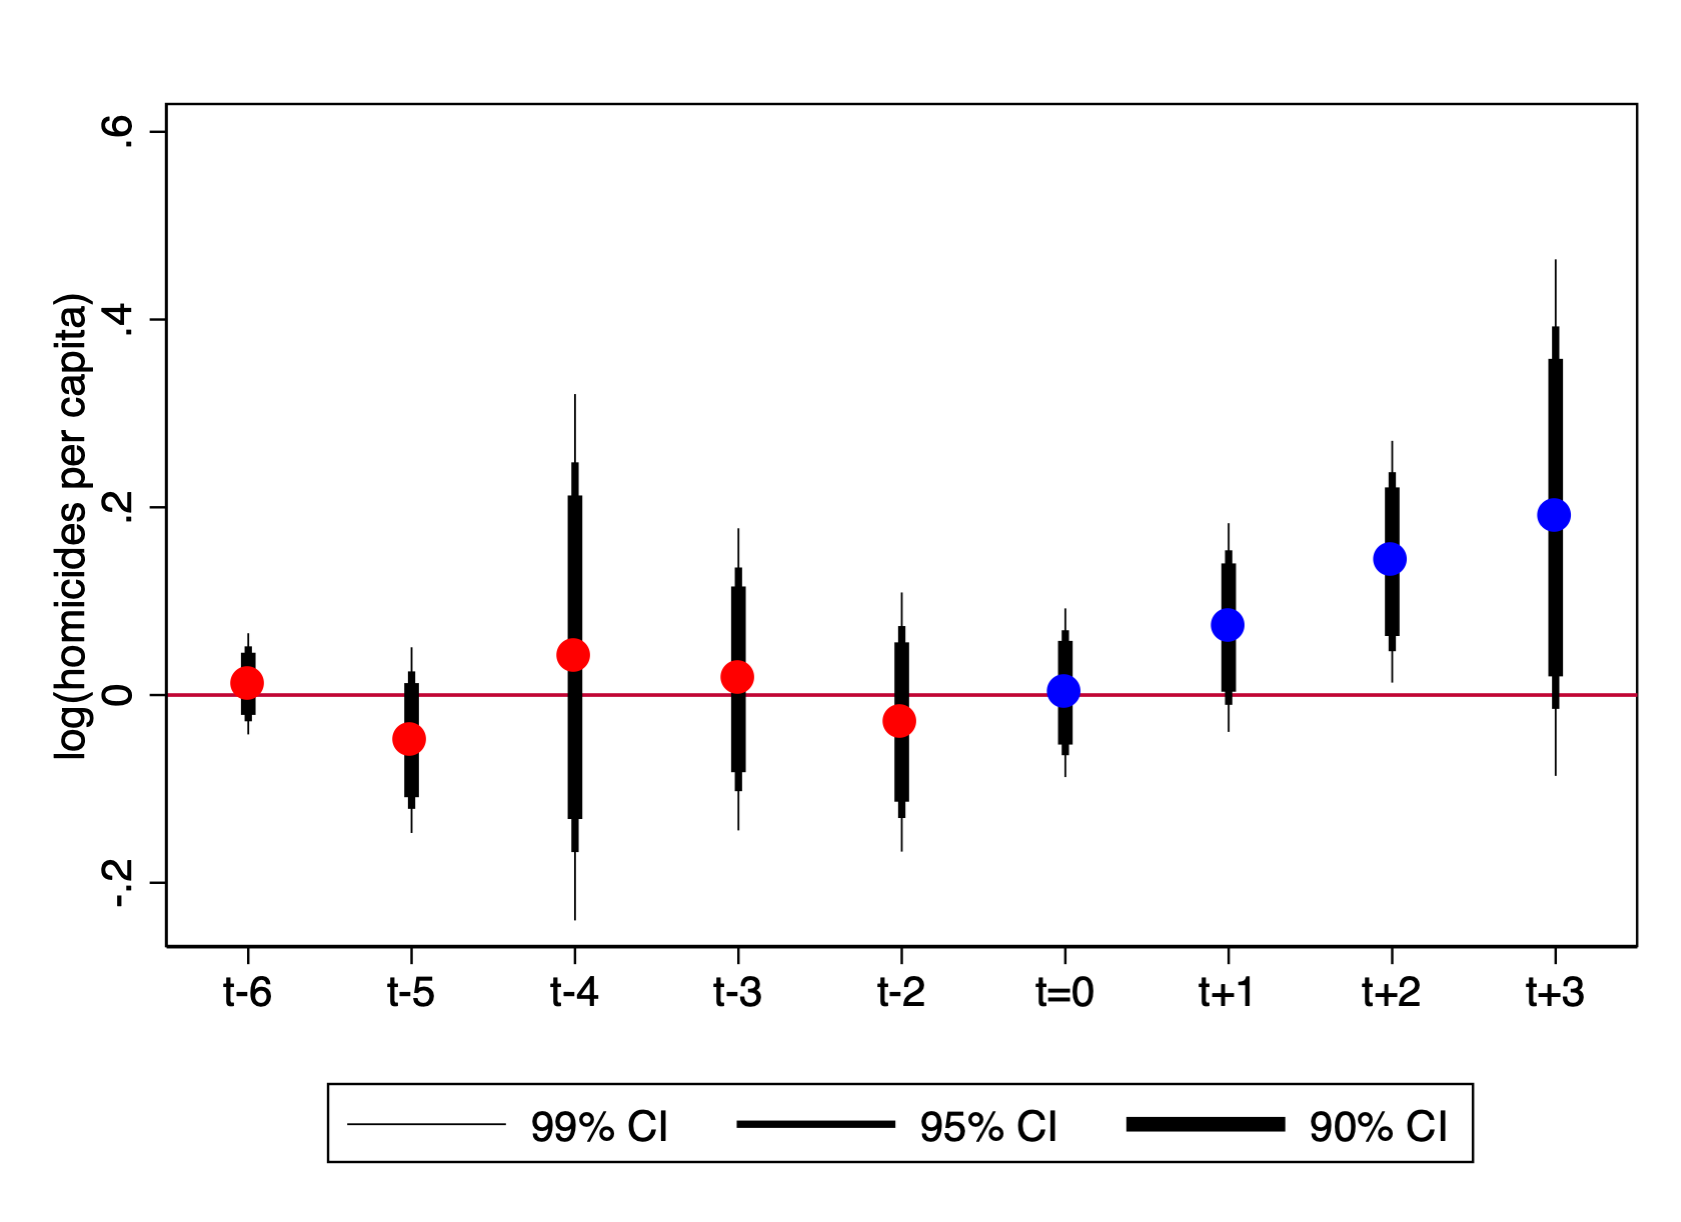
\includegraphics[width=0.9\textwidth]{Figures/catts_homicides.png}
       \captionsetup{justification=centering}
       
 \textbf{Note:} Figure \ref{fig:as_violence} shows the IW estimators following \citet{abraham_sun_2020} for each lead and lag relative to the first year a municipality implemented reelection. Red points are pre-treatment, while blue ones post-treatment. 
    
\end{figure}    
     

What are the results of not delegating security policy to more capable agents like the governor? Until now, I have assumed that the public security provision is a more efficient endeavor under the hands of governors who can pool a greater amount of resources, information, skills and expertise than mayors. Moreover, given the high presence of spillovers delegation seems to be the most efficient way to achieve the monopoly of violence \citep{oates_1972}. Figure \ref{fig:as_violence} reports the IW estimator for each lead and lag relative to the first year a municipality implemented reelection. Results show a disastrous backlash from reelection incentives. On average, from $t$ to $t+3$, homicides per capita increased in 10.4\% using a logarithmic transformation and 6.6\% using the inverse hyperbolic transformation, significant to the 5 and 10\% respectively. As Appendix Figure \ref{fig:robustness_violence} shows, results are robust across multiple specifications including changing the reference period of the reform and adjusting for the small number of clusters (states) using Wild bootstraps. Further validation is provided by the use of \citet{imai_etal_2020} non-parametric generalization of the difference-in-difference estimator that corrects for invalid negative weighting in standard two-way fixed effects models through propensity score matching (see Appendix Figure \ref{fig:matching_violence}). 

One concern could be that while the Term Limit Reform increased the level of violence in the reduced form specification, the decrease in agreements might not be the explaining mediator. To validate delegation as a mechanism for violence, Table \ref{tab:2sls_agreement_violence} shows a two-stage least squares model where agreements are instrumented by the Term Limit Reform using the cohort-weighted event study design of Figure \ref{fig:event_study_agreements}.\footnote{\citet{mostad_etal_2020} have raised concerns that the two-stage least squares with multiple instrumental variables might yield biased results in the presence of heterogeneous treatment effects. However, since we take care of this by relying on the cohort-weighted event study design by \citet{abraham_sun_2020}.} The table shows that the delegation of security policy to governors decreases violence by 15.2 percentage points, significant to the 5\% level when including state-clustered standard errors corrected for the small number of clusters using wild bootstrap. In other words, a decrease in the delegation of security policy increases violence. 
   
    
\begin{table}[h]\def\sym#1{\ifmmode^{#1}\else\(^{#1}\)\fi}
\centering
\caption{Effect of Security Cooperation Agreements signed with the Governor on Violence}
\label{tab:2sls_agreement_violence}
\scalebox{0.7}{
\begin{tabular}{l*{2}{c}}
\hline \hline
\multicolumn{3}{l}{Dependent variable: log(homicides per capita)} \\
  &\multicolumn{1}{c}{(1)}         &\multicolumn{1}{c}{(2)}         \\
\addlinespace
Predicted Agreement w/ Governor&     -0.1521\sym{*}  &     -0.1521\sym{**} \\
            &    (0.0802)         &    (0.0749)         \\
\addlinespace
Observations&      12,173         &      12,173         \\
R2          &       0.724         &       0.724         \\
Controls$^a$    &  \checkmark         &  \checkmark         \\
Mun. FE     &  \checkmark         &  \checkmark         \\
Year FE     &  \checkmark         &  \checkmark         \\
State Cluster S.E.&                     &  \checkmark         \\
Wild CI$^b$     &                     &  \checkmark         \\
First stage F-stat      &        1,739         &        1,739         \\
\hline \hline
\multicolumn{3}{p{0.7\textwidth}}{\footnotesize{Notes: Coefficients show IW estimators following \citet{abraham_sun_2020}. Two relative time periods (lag 8 and 1) were removed to avoid collinearity problems noted by \citet{abraham_sun_2020}. Standard errors in parentheses are clustered at the state level unless indicated, with the following significance-level: $^{***}$ 1\%; $^{**}$ 5\%; and $^*$ 10\%, that refer to two-sided t-test with the null hypothesis equal to 0 for each relative time period.  $^a$ Pretreatment controls include: governor winning margin; party alignment with the President;  party alignment with the Governor; municipal winning margin; and Cartel presence. $^a$ Wild bootstrap standard errors clustered at the state-level are reported when indicated.}} \\
\end{tabular}
}
\end{table} 

\begin{figure}[H]  
\centering
\caption{Effect of Term Limit Reform on Effort of Local and Federal Security Forces} 
\label{fig:effort}

   
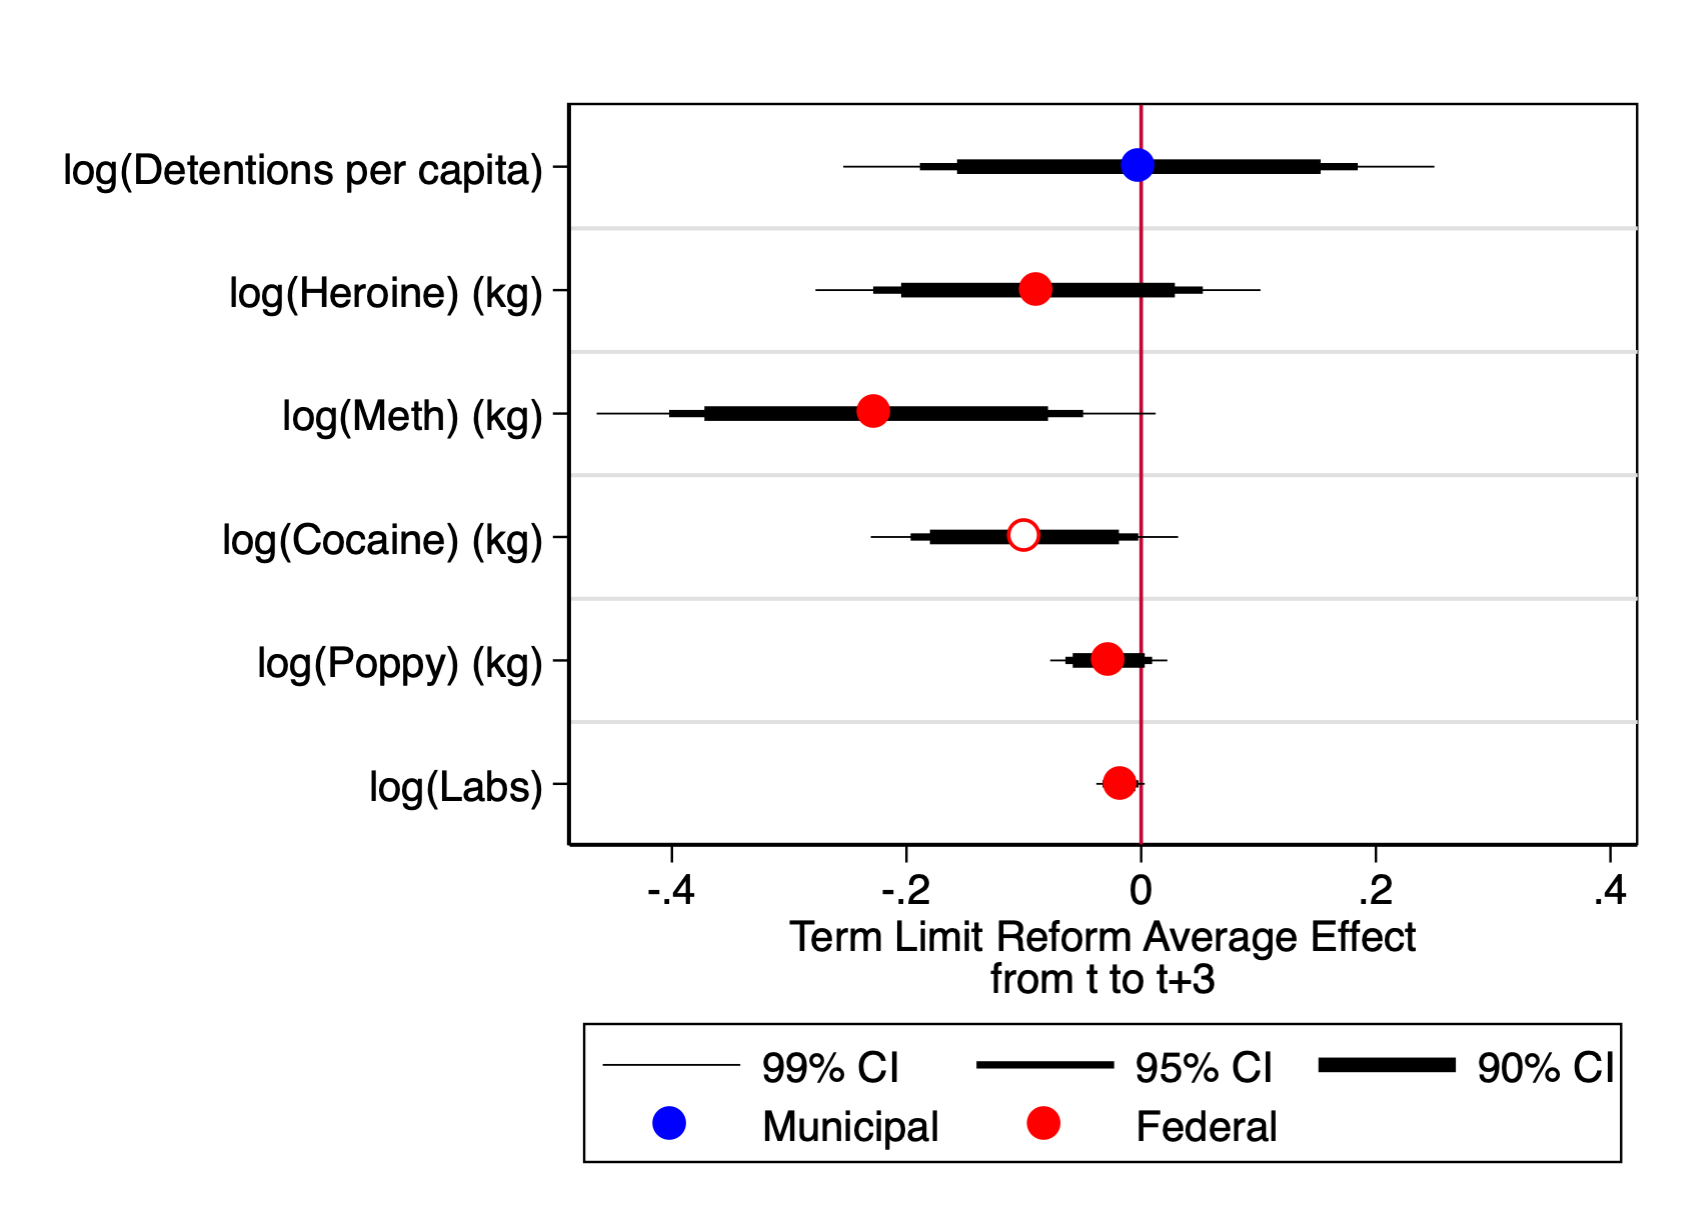
\includegraphics[width=0.75\textwidth]{Figures/effort.png}
  
 \textbf{Note:} Figure \ref{fig:effort} shows the average treatment effect from t to t+3 across multiple specifications. This average effect was estimated using the IW estimators following \citet{abraham_sun_2020} for each lead and lag relative to the first year a municipality implemented reelection. Filled points show that parallel trends hold, while hollow ones imply pretrends.        
\end{figure} 


Is the level of effort placed by incumbents seeking reelection explaining this increase in violence? Figure \ref{fig:effort} shows that while the effort placed by the local police in municipalities with mayors seeking reelection remains similar to that of term-limited incumbents as measured by the number of detentions per capita made by the municipal police, we observe a decrease in anti-narcotic activities by federal and state-level forces. In other words, municipalities that do not delegate security provision are left to their luck to fight crime. 


 
\section{Conclusion \label{sec:conclusion}}

This paper studies a classic problem faced by governments with a supra-entity capable of providing and delivering public goods: to delegate or not to delegate. Specifically, it delves into an understudied phenomenon of delegation, the role of reelection incentives. I find that reelection encourages mayors to focus on policies with the highest “electoral yield”—namely, not to delegate public security to the governor. Why? By directly delivering public security mayors are responsiveness to citizens and signal a competent type to voters. This behavior is predominant when citizens are concerned about narcotraffic and when citizens are capable of blaming or rewarding local politicians, i.e. when incumbents seeking reelection are aligned with the party of the governor. Since delegation of local security policy to the governor is the most efficient choice in this setting, reelection incentives lead to an inefficient outcome: an increase in violence. These results suggests that reelection incentives may lead incumbents to differentiate themselves by tacking charge of policy at the expense of inefficiency. This makes delegation not only a political but an electoral decision. 
  
    
            
%BIBLIOGRAPHY -----------------------------------------------
\clearpage
   
%%%%%%%%%%%%
\bibliographystyle{aer} 
\bibliography{References}      

\clearpage
%APPENDIX -----------------------------------------------
\begin{appendix}


%%%%%%%%% Electoral Reform 2014
\section{Political Background of the 2014 Electoral Reform}\label{appendix:reform_backgorund}


It is important to understand the electoral reform political motivation, which involved a bargaining process with the opposition as well as the incorporation of pending laws from the political reform of 2012 under the PAN presidency. In the last year of Felipe Calderon presidency, a political reform was introduced in Congress including a term limit removal for all political actors. This reform was proposed and introduced during the electoral period of that year, increasing political tensions among the incumbent and opposition parties. The PRI -at the time part of the opposition and in control of the lower legislative house- blocked the reform and targeted reelection and the introduction of a second electoral round for the presidential election. 
 
  The 2012 presidential election was won by the coalition ``Alliance for Mexico'' with its presidential candidate Enrique Pena Nieto.\footnote{The PRI won with 38.2\% of total votes, followed by the PRD with 32.6\% and the PAN with 25.390\%.} However, the election suffered multiple electoral irregularities exposed by the national media. Among anomalies, opposition parties led by Andres Manuel Lopez Obrador -the second runner of presidential election and at the time presidential candidate for the left-wing party PRD-, argued PRI's financial expenses above campaign caps and vote-buying practices including the distribution of gift cards from several institutions, including one of the country's largest supermarket chains, Soriana, to voters in the State of Mexico and Mexico city. \citet{cantu_2019} finds not only an effect of the gift cards in PRI electoral return, but a magnitude that increases given proximity of electoral precincts to stores. While the special commission in the Chamber of Deputies found that the PRI invested \$5,200 million pesos in the campaign, an amount 15 times larger than the finance cap of \$336 million pesos, and the Inspection Unit from the Federal Electoral Institute (IFE for its acronym in Spanish) detailed the financing network where Soriana, Banamex, Monex and other firms where involved, the Unit did not point to any law violation. Without a public discussion, the ministers of the Federation Judicial Electoral Tribunal (TEPJF for its acronym in Spanish) deemed the appeal filed by the PRD unfounded and endorsed IFE's  criterion that the PRI was not obliged to register the agreement with Soriana, Banamex or Monex as campaign expenses.\footnote{In his presentation, magistrate Manuel Gonzalez Oropeza stated that the analysis carried by the Inspection Unit showed that ``neither the allegedly hidden financing was accredited individually or jointly" by any member of the PRI. See \url{https://www.jornada.com.mx/2013/01/24/politica/013n2pol} for more detail.} The final resolution of IFE's Council and the TEPJF increased citizens and opposition mistrust on electoral institutions. 

By early 2013, the Pena Nieto administration pushed an aggressive set of reforms to privatize the energy sector and modify the existent fiscal institutions in the country. To increase the probability of success, the PRI with the PAN and PRD, the three main political parties at the time, lead the construction of the Mexican Pact Accord, a series of roundtables intended to negotiate the energy sector reform along a set of structural reforms that had fail to pass through congress due to political gridlocks.\footnote{The PRD was no longer under the Lopez Obrador leadership who left the party to build a new left-wing party called MORENA once the leaders from the PRD agreed to form part of the Mexican Pact Accord.} While the Electoral Reform was not under PRI's set of desired reforms, the opposition utilize it as a bargaining chip to approve those pursued by the PRI \citep{zamitiz_2017}. By the end of May 2013, a roundtable to discuss the electoral reform was installed. Specifically, commitment 94 of the Pact Accord introduced reelection for discussion. However, due to lack of consensus, the Mexican Pact Accord did not submit an electoral reform proposal to Congress and left the bargaining process to the Senate. Two months later, on July 24, 2013, PAN and PRD pushed a political-electoral reform with 36 law changes that included  the creation of a National Electoral Institute (INE for its acronym in Spanish) that would be in charge of federal, state and local elections and reelection for federal and local legislators and mayors. In the words of the current Chairman of the INE, Lorenzo Cordova, ``[w]ith the reform, we went from an electoral model made up of a federal electoral system and thirty-two electoral systems, to a national election system in which a national authority and thirty-two local authorities coexist; a national administrative body was created, with clear powers and powers for local elections, and an authority was created that coordinates and guarantees the same parameters for the application of laws by local authorities, in order to standardize the conditions of the electoral competition in all elections and to promote a more transparent and impartial democracy throughout the country€.\footnote{From Cfr. Compendio de Legislacion Nacional Electoral, Mexico, INE, FEPADE, UNAM, TEPJF, Tomo II, 2014, p. XXXIX.} 


The reaction of governors was not smooth since reelection would limit the influence of governors and local elites on the electoral processes of the 32 states. Strong governors like the priista Eruviel Avila Villegas from the State of Mexico labeled this initiative as ``democratic regression".\footnote{For more detail see ``Regresion democratica, creacion del Instituto Nacional de Elecciones€, La Jornada, 30 de octubre, 2013, p. 15. \url{https://www.20minutos.com.mx/noticia/b82075/regresion-democratica-creacion-del-instituto-nacional-de-elecciones/}} Given the state-level opposition, Senate leaders from the PAN and PRD chose to approve the electoral reform in December 2, 2013, before the energy reform, and thus increased their political grip over the PRI.\footnote{The electoral reform approved by the Senate included reelection for federal legislators and governors for up to 12 years, as well as reelection for local legislators and mayors. Congress, however, modified the proposal removing governors reelection. The electoral reform was approved with 408 votes in favor and 69 against in Congress on December 3, 2013, and weeks later by the Senate due to modifications of the original reform project.} By January 2014, PAN and PRD threatened to back the energy reform  if the PRI did not push local state legislatures from approving the electoral reform, a constraint imposed by the Mexican constitution, which at the time where blocking the reform given pressure from various PRI governors.\footnote{For more detail see Enrique Mendez, ``PAN: estancados, cambios en materia politica por presion de los gobernadores€, La Jornada, 9 de enero de 2014, p. 5., \url{https://jornada.com.mx/2014/01/09/politica/005n3pol}.} The political gridlock led former President Pena Nieto to ``exhort" local legislators to approve the electoral reform. On January 31, 2014, the reform was promulgated by the President and contained three main changes: (1) the creation of the INE; (2) removal of term limits of mayors, local and federal legislators for up to 2 terms; (3) the introduction of a ``party-lock"	where mayors or legislators who wish to reelected could not switch parties. As a result, while voter accountability increased, party control remained unchanged since candidate nominations and campaign funding still depended strongly on them. 
 \clearpage 
  
%%%%%%%%%%%%%%%%%%%%%%%%%%%%%%%%%%%%

\renewcommand{\thetable}{B-\arabic{table}}
\setcounter{table}{0}
 
 \renewcommand{\thefigure}{B-\arabic{figure}}
\setcounter{figure}{0}

\clearpage
\section{Additional Tables and Figures \label{sec:additional_tables}}

\subsection{Descriptive Statistics}

%Table
\begin{table}[H]
\centering 
\caption{Descriptive statistics}
 
\label{tab:descriptive}
\scalebox{0.65}{ 
{
\def\sym#1{\ifmmode^{#1}\else\(^{#1}\)\fi}
\begin{tabular}{l*{1}{ccccc}}
\hline\hline
            &        \textbf{Mean}&  \textbf{SD}&  \textbf{Min}&  \textbf{Max}& \textbf{N}\\
\hline
\emph{Pane A - Security Cooperation Agreements:} 	&		&		&		&		\\
Security Coop. Agreement with governor&        0.28&        0.45&           0&           1&      17,832\\
Security Coop. Agreement with other actors besides the governor&        0.06&        0.24&           0&           1&       6,466\\
Delegate Public Security Provision&        0.29&        0.45&           0&           1&       7,123\\
Delegate Transit Activities&        0.10&        0.30&           0&           1&       7,123\\
Delegate Training of Police Forces&        0.08&        0.27&           0&           1&       4,750\\
Delegate Equipment and Technology&        0.08&        0.26&           0&           1&       4,750\\
Delegate Research Activities&        0.07&        0.26&           0&           1&       4,750\\
Delegate Intelligence Activities&        0.07&        0.26&           0&           1&       4,750\\
Delegate the Unification of Laws and Procedures&        0.08&        0.27&           0&           1&       4,750\\
Delegate Public Security Prevention&        0.08&        0.27&           0&           1&       4,750\\
Reason to delegate: Constitutional Change&        0.12&        0.33&           0&           1&      14,248\\
Reason to delegate: Change in Local Laws&        0.11&        0.31&           0&           1&      14,248\\
Reason to delegate: Constitutional Change&        0.11&        0.31&           0&           1&      14,248\\
Reason to delegate: Need of Professionalization&        0.12&        0.33&           0&           1&      14,248\\
Reason to delegate: Need of Coordination&        0.17&        0.38&           0&           1&      14,248\\
Reason to delegate: Prevalence of Crime&        0.09&        0.29&           0&           1&      14,248\\
Reason to delegate: Other&        0.07&        0.25&           0&           1&      14,248\\


\\
\emph{Panel B - Violence:} 	&		&		&		&		\\
deaths by homicide per capita (INEGI)&       23.99&      128.24&           0&       8,462&      21,375\\
log(deaths by homicide per capita) (INEGI)&       -8.34&        1.04&         -13&        -2.4&      21,375\\
asinh(deaths by homicide per capita) (INEGI)&        2.33&        1.91&           0&         9.7&      21,375\\

\\
\emph{Panel C - Citizens' Preferences:} 	&		&		&		&		\\
Topic that worries most: narcotraffic (for all years)&        0.15&        0.05&           0&         .37&      16,625\\
Topic that worries most: insecurity (for all years)&        0.56&        0.09&           0&         .77&      16,625\\
Topic that worries most: punishment of criminals (for all years)&        0.17&        0.06&           0&         .38&      16,625\\
Topic that worries most: corruption (for all years)&        0.26&        0.04&           0&         .36&      16,625\\
Topic that worries most: poverty (for all years)&        0.34&        0.07&           0&         .52&      16,625\\
Topic that worries most: unemployment (for all years)&        0.40&        0.07&           0&         .57&      16,625\\
Topic that worries most: inflation (for all years)&        0.35&        0.04&           0&         .46&      16,625\\
Topic that worries most: natural disaster (for all years)&        0.05&        0.02&           0&         .12&      16,625\\
Topic that worries most: water scarcity (for all years)&        0.15&        0.04&           0&         .25&      16,625\\
Topic that worries most: health (for all years)&        0.23&        0.03&           0&         .31&      16,625\\
Topic that worries most: education (for all years)&        0.31&        0.05&           0&         .47&      16,625\\

\\
\emph{Panel D - Incumbents' quality:} 	&		&		&		&		\\
Incumbent undergraduate or graduate title (indicator)&        0.06&        0.24&           0&           1&      19,430\\

\\ 
%\emph{Pane B - 2014 Electoral Reform:} 	&		&		&		&		\\
%rel\_year==    -8.0000&        0.02&        0.13&           0&           1&      18,000\\
rel\_year==    -7.0000&        0.02&        0.14&           0&           1&      18,000\\
rel\_year==    -6.0000&        0.06&        0.24&           0&           1&      18,000\\
rel\_year==    -5.0000&        0.11&        0.31&           0&           1&      18,000\\
rel\_year==    -4.0000&        0.11&        0.31&           0&           1&      18,000\\
rel\_year==    -3.0000&        0.11&        0.31&           0&           1&      18,000\\
rel\_year==    -2.0000&        0.11&        0.31&           0&           1&      18,000\\
rel\_year==    -1.0000&        0.11&        0.31&           0&           1&      18,000\\
rel\_year==     0.0000&        0.11&        0.31&           0&           1&      18,000\\
rel\_year==     1.0000&        0.09&        0.29&           0&           1&      18,000\\
rel\_year==     2.0000&        0.09&        0.29&           0&           1&      18,000\\
rel\_year==     3.0000&        0.05&        0.22&           0&           1&      18,000\\


%\\

\\ 
 

\hline\hline
\multicolumn{6}{p{1.3\textwidth}}%{\footnotesize{Note: .        
 % }} \\  

\end{tabular} 
} 
}
\end{table}

\pagebreak

%Table
\begin{table}[H]
\centering 
\caption{Descriptive statistics (continuation)}
 
\label{tab:descriptive2}
\scalebox{0.65}{ 
{
\def\sym#1{\ifmmode^{#1}\else\(^{#1}\)\fi}
\begin{tabular}{l*{1}{ccccc}}
\hline\hline
            &        \textbf{Mean}&  \textbf{SD}&  \textbf{Min}&  \textbf{Max}& \textbf{N}\\
\hline

\emph{Panel E - Mechanisms:} 	&		&		&		&		\\
Topic that worries most: narcotraffic (average pre-treatment)&        0.15&        0.05&           0&         .27&      21,375\\
Topic that worries most: insecurity (average pretreatment)&        0.52&        0.08&           0&         .68&      21,375\\
Topic that worries most: punishment of criminals (average pretreatment)&        0.12&        0.02&           0&         .19&      21,375\\
Topic that worries most: poverty (average pretreatment)&        0.37&        0.07&           0&          .5&      21,375\\
Topic that worries most: unemployment (average pretreatment)&        0.46&        0.04&           0&         .52&      21,375\\
Topic that worries most: inflation (average pretreatment)&        0.37&        0.03&           0&         .41&      21,375\\
Topic that worries most: natural disaster (average pretreatment)&        0.05&        0.01&           0&        .088&      21,375\\
Topic that worries most: water scarcity (average pretreatment)&        0.15&        0.03&           0&          .2&      21,375\\
Topic that worries most: corruption (average pretreatment)&        0.24&        0.04&           0&         .34&      21,375\\
Topic that worries most: health (average pretreatment)&        0.24&        0.03&           0&         .29&      21,375\\
Topic that worries most: education (average pretreatment)&        0.31&        0.06&           0&          .4&      21,375\\
Trust in Municipal Security Forces&        0.21&        0.05&           0&          .4&      21,375\\
Trust in State Security Forces&        0.22&        0.05&           0&         .37&      21,375\\
Trust in Federal Security Forces, including the military&        0.55&        0.16&           0&         .77&      21,375\\
Identify Municipal Security Forces&        0.70&        0.06&           1&         .87&      21,375\\
Identify State Security Forces&        0.51&        0.07&           0&          .7&      21,375\\
Identify Federal Security Forces, including the military&        0.53&        0.08&           0&         .75&      21,375\\
Corruption of Municipal Security Forces&        1.24&        0.15&           1&         1.7&      21,375\\
Corruption of State Security Forces&        1.24&        0.14&           1&         1.6&      21,375\\
Corruption of Federal Security Forces, including the military&        1.07&        0.14&           1&         1.6&      21,375\\
Efficiency of Municipal Security Forces&        0.24&        0.06&           0&         .42&      21,375\\
Efficiency of State Security Forces&        0.25&        0.06&           0&         .41&      21,375\\
Efficiency of Federal Security Forces, including the military&        0.57&        0.15&           0&         .78&      21,375\\
Detained by local police per capita (in flagrancy, SNSP)&       10.29&      133.10&           0&      11,408&      21,375\\
log(Detained by local police per capita) (in flagrancy, SNSP)&       -9.06&        1.32&         -14&        -2.2&      21,375\\
log(heroine kg), SEDENA&        0.01&        0.15&           0&         5.4&      21,375\\
log(meth kg), SEDENA&        0.05&        0.48&           0&          10&      21,375\\
log(cocaine kg), SEDENA&        0.04&        0.36&           0&         7.8&      21,375\\
log(poppy kg), SEDENA&        0.19&        0.82&           0&         8.8&      21,375\\
log(laboratories erradicated), SEDENA&        0.02&        0.17&           0&         4.1&      21,375\\
 
\\
\emph{Panel F - Controls:} 	&		&		&		&		\\
Population (INEGI and CONAPO projections)&      53,389&     141,924&         409&   1,714,709&       2,227\\
 
Winning margin: first - second runner (governor)&        0.15&        0.13&           0&           1&      21,375\\
alignment with federal executive=1; 0 otherwise&        0.77&        0.42&           0&           1&      17,962\\
alignment with state executive=1; 0 otherwise&        0.37&        0.48&           0&           1&      17,962\\
Winning margin: first - second runner&        0.11&        0.11&           0&           1&      17,962\\
PAN mayor=1; 0 otherwise&        0.29&        0.46&           0&           1&      17,962\\
PRI mayor=1; 0 otherwise&        0.46&        0.50&           0&           1&      17,962\\
Incidence of Cartel Presence&        0.22&        0.35&           0&           1&      21,375\\

\\ 
 
    
\hline\hline
\multicolumn{6}{p{1.3\textwidth}}%{\footnotesize{Note: .        
 % }} \\  

\end{tabular} 
} 
}
\end{table}

\pagebreak
   
\subsection{Main Results}
\begin{table}[H]\def\sym#1{\ifmmode^{#1}\else\(^{#1}\)\fi}
\centering
\caption{Effect of 2014 Term Limit Reform on Security Cooperation Agreements signed with the Governor, 2010-2018}
\label{tab:as_agreements}
\scalebox{0.75}{
\begin{tabular}{lcc}
\hline \hline
\\ \multicolumn{3}{l}{Dependent variable:}\\
& \multicolumn{2}{c}{Security Cooperation Agreement} \\
& \multicolumn{2}{c}{w/ Governor$^{a}$} \\

& \multicolumn{1}{c}{(1)} & \multicolumn{1}{c}{(2)} \\
\cmidrule(lrr){2-2}  \cmidrule(lrr){3-3}\\
\addlinespace
Lag 7 years &      $ 0.1123^{} $ &  $ 0.1123^{} $   \\
& ($ 0.1709$) & ($ 0.7117 $) \\
Lag 6 years &          $ -0.0383^{} $ &   $ -0.0383^{} $  \\
& ($ 0.0579$) & ($ 0.2458 $) \\
Lag 5 years &        $ -0.0848^{} $ &   $ -0.0848^{} $ \\
& ($ 0.0846$) & ($ 0.2404 $) \\
Lag 4 years &         $ 0.0751^{} $ &      $ 0.0751^{} $  \\
& ($ 0.3174$) & ($ 0.2890 $) \\
Lag 3 years &        $ 0.2088^{} $ &     $ 0.2088^{} $ \\
& ($ 0.2603$) & ($ 0.2139 $) \\
Lag 2 years &        $ 0.0044^{} $ &    $ 0.0044^{} $  \\
& ($ 0.1583$) & ($ 0.2139 $) \\
Reform, time 0 &        $ -0.2446^{***} $ &     $ -0.2446^{***} $ \\
& ($ 0.0475$) & ($ 0.0685 $) \\
Lead 1 year &         $ -0.4154^{***} $ &       $ -0.4154^{***} $ \\
& ($ 0.0610$) & ($ 0.0610 $) \\
Lead 2 years &         $ -0.4259^{***} $ &      $ -0.4259^{***} $  \\
& ($ 0.0571$) & ($ 0.0571 $) \\
Lead 3 years &        $ -0.5931^{***} $ &     $ -0.5931^{***} $ \\
& ($ 0.0604$) & ($ 0.0604 $) \\
\addlinespace
Observations       &                 12,173        &          12,173  \\
R-squared        &              0.4545        &           0.4545   \\
Mun. FEs       &     \checkmark         &  \checkmark    \\
Year. FEs       &     \checkmark         &  \checkmark   \\
Controls$^b$   &      \checkmark       &      \checkmark    \\
Cohort weighted   &   \checkmark       &   \checkmark    \\
WILD CI   &          &   \checkmark    \\
Aggregate effect        &           $   -0.4197^{***} $        &           $-0.4197^{***} $    \\
SE (aggregate eff.)        &              0.0457        &           0.0473   \\
\hline \hline
\multicolumn{3}{p{0.6\textwidth}}{\footnotesize{Notes: Coefficients show IW estimators following \citet{abraham_sun_2020}. Two relative time periods (lag 8 and 1) are removed to avoid collinearity problems noted by \citet{abraham_sun_2020}. Standard errors in parentheses are clustered at the state level, with the following significance-level: $^{***}$ 1\%; $^{**}$ 5\%; and $^*$ 10\%, that refer to two-sided t-test with the null hypothesis equal to 0 for each relative time period. $^a$ Refers to security cooperation agreements signed with the Governor. $^b$ Pretreatment controls include: governor winning margin; party alignment with the President;  party alignment with the Governor; municipal winning margin; logged population; logged organized crime related deaths; and Cartel presence.}} \\
\end{tabular}
} 
\end{table}
    
 
 \clearpage
\subsection{Robustness}

\begin{table}[htbp]\def\sym#1{\ifmmode^{#1}\else\(^{#1}\)\fi}
\centering
\caption{Effect of 2014 Term Limit Reform on Signing Security Cooperation Agreements, Average Effect }
\label{tab:as_aggregate}
\scalebox{0.7}{
\begin{tabular}{lcccc}
\hline \hline
\\ \multicolumn{3}{l}{Dependent variable: Sign Security Cooperation Agreement w/ Governor}\\
Model: & CATTs & CATTs w/ WILD CIs & Change ref. period (t=0) & Trim $<$ t-4 \\
& \multicolumn{1}{c}{(1)} & \multicolumn{1}{c}{(2)} & \multicolumn{1}{c}{(3)}  & \multicolumn{1}{c}{(4)}  \\
\cmidrule(lrr){2-2}  \cmidrule(lrr){3-3}  \cmidrule(lrr){4-4} \cmidrule(lrr){5-5}\\
\addlinespace
Reform Average Effect (from t to t+3)       & $-0.4197^{***} $$ & $-0.4197 ^{***} $$ & $-0.4622 ^{**} $$ & $-0.3559 ^{***} $$   \\
& (0.0457( & (0.0473)  & (0.1977) & (0.0468)  \\
\addlinespace
Observations       &      12,173 &      12,173 &      12,173 &      12,173 \\
R-squared         & 0.4545 & 0.4545 & 0.4545 & 0.4544 \\
Mun. FEs       &     \checkmark         &  \checkmark &     \checkmark         &  \checkmark     \\
Year. FEs       &     \checkmark         &  \checkmark  &     \checkmark         &  \checkmark \\
Controls$^b$   &      \checkmark       &      \checkmark &      \checkmark       &      \checkmark    \\
Cohort weighted   &   \checkmark       &   \checkmark  &   \checkmark       &   \checkmark  \\
Parallel trend holds   &   \checkmark       &   \checkmark  &   \checkmark       &   \checkmark   \\
\hline \hline
\multicolumn{5}{p{1.3\textwidth}}{\footnotesize{Notes: Coefficients show IW estimators following \citet{abraham_sun_2020}. Two relative time periods (lag 8 and 1) are removed to avoid collinearity problems noted by \citet{abraham_sun_2020} except for the specification that trims periods prior to t-4. Standard errors in parentheses are clustered at the state level, with the following significance-level: $^{***}$ 1\%; $^{**}$ 5\%; and $^*$ 10\%, that refer to two-sided t-test with the null hypothesis equal to 0 for each relative time period. $^b$ State-level controls include governor winning margin in last pre-treatment election and an indicator of whether the governor's party is the same as the federal incumbent party.}} \\
\end{tabular}
}
\end{table}
 

\begin{table}[htbp]\def\sym#1{\ifmmode^{#1}\else\(^{#1}\)\fi}
\centering
\caption{Effect of 2014 Term Limit Reform on the likelihood of signing Security Cooperation Agreements, \citet{chaisemarting_etal_2019} correction}
\label{tab:chaisemartin_agreements}
\scalebox{1}{
\begin{tabular}{lcc}
\hline \hline
\\ \multicolumn{3}{l}{Dependent variable:}\\
& \multicolumn{1}{c}{Agreement A} & \multicolumn{1}{c}{Agreement B$^{a}$} \\
& \multicolumn{1}{c}{(1)} & \multicolumn{1}{c}{(2)} \\
\cmidrule(lrr){2-2}  \cmidrule(lrr){3-3}\\
\addlinespace
t-6 &          $ -0.0645^{} $ &   $ -0.0645^{} $  \\
& ($ 0.0399$) & ($ 0.8961 $) \\
t-5 &        $ -0.2071^{**} $ &   $ -0.2071^{} $ \\
& ($ 0.0751$) & ($ 2.6703 $) \\
t-4 &         $ -0.0712^{} $ &      $ -0.0712^{} $  \\
& ($ 0.1733$) & ($ 1.2658 $) \\
t-3 &        $ 0.1037^{} $ &     $ 0.1037^{} $ \\
& ($ 0.1362$) & ($ 0.3138 $) \\
t-2 &        $ -0.0251^{} $ &    $ -0.0251^{} $  \\
& ($ 0.1157$) & ($ 0.3138 $) \\
t-1 &        $ -0.0738^{} $ &     $ -0.0738^{} $ \\
& ($ 0.0918$) & ($ 1.6557 $) \\
t+1 &         $ -0.2837^{} $ &       $ -0.2837^{} $ \\
& ($ 0.2012$) & ($ 0.2012 $) \\
t+2 &         $ -0.6165^{**} $ &      $ -0.6165^{**} $  \\
& ($ 0.2330$) & ($ 0.2330 $) \\
t+3 &        $ -0.4813^{*} $ &     $ -0.4813^{*} $ \\
& ($ 0.2641$) & ($ 0.2641 $) \\
\addlinespace
Observations       &                 12,173        &          12,173  \\
R-squared        &              0.4542        &           0.4542   \\
Mun. FEs       &     \checkmark         &  \checkmark    \\
Year. FEs       &     \checkmark         &  \checkmark   \\
Controls$^b$   &      \checkmark       &      \checkmark    \\
Cohort weighted   &   \checkmark       &   \checkmark    \\
WILD CI   &          &   \checkmark    \\
Aggregate effect        &              -0.4605        &           -0.4605   \\
SE (aggregate eff.)        &              0.1973        &           0.1973   \\
p-value(aggregate eff.)       &              0.0273        &           0.0273   \\
\hline \hline
\multicolumn{3}{p{0.8\textwidth}}{\footnotesize{Notes: Coefficients show IW estimators following \citet{abraham_sun_2020}. Two relative time periods (lag 8 and 1) are removed to avoid collinearity problems noted by \citet{abraham_sun_2020}. Standard errors in parentheses are clustered at the state level, with the following significance-level: $^{***}$ 1\%; $^{**}$ 5\%; and $^*$ 10\%, that refer to two-sided t-test with the null hypothesis equal to 0 for each relative time period. $^a$ Refers to the inverse hyperbolic sine transformation. $^b$ State-level controls include governor winning margin in last pre-treatment election and an indicator of whether the governor's party is the same as the federal incumbent party.}} \\
\end{tabular}
}
\end{table}
  
    
 \begin{table}[htbp]\def\sym#1{\ifmmode^{#1}\else\(^{#1}\)\fi}
\centering
\caption{Effect of Term Limit Reform on Security Cooperation Agreements signed with the Governor, trimming periods}
\label{tab:as_agreements_trim}
\scalebox{1}{
\begin{tabular}{lcc}
\hline \hline
\\ \multicolumn{3}{l}{Dependent variable:}\\
& \multicolumn{2}{c}{Security Cooperation Agreement} \\
& \multicolumn{2}{c}{w/ Governor$^{a}$} \\
& \multicolumn{1}{c}{(1)} & \multicolumn{1}{c}{(2)} \\
\cmidrule(lrr){2-2}  \cmidrule(lrr){3-3}\\
\addlinespace
t-4 years &         $ 0.1961^{} $ &      $ 0.1961^{} $  \\
& ($ 0.2680$) & ($ 0.8260 $) \\
t-3 &        $ 0.2193^{} $ &     $ 0.2193^{} $ \\
& ($ 0.2070$) & ($ 0.2702 $) \\
t-2 &        $ 0.0370^{} $ &    $ 0.0370^{} $  \\
& ($ 0.1546$) & ($ 0.2702 $) \\
t=0 (Reform) &        $ -0.3057^{***} $ &     $ -0.3057^{} $ \\
& ($ 0.0682$) & ($ 0.4093 $) \\
t+1 &         $ -0.2858^{***} $ &       $ -0.2858^{} $ \\
& ($ 0.0725$) & ($ 0.2610 $) \\
t+2 &         $ -0.2389^{***} $ &      $ -0.2389^{} $  \\
& ($ 0.0823$) & ($ 0.2369 $) \\
t+3  &        $ -0.5931^{***} $ &     $ -0.5931^{***} $ \\
& ($ 0.0604$) & ($ 0.0715 $) \\
\addlinespace
Observations       &                 12,173        &          12,173  \\
R-squared        &              0.4544        &           0.4544   \\
Mun. FEs       &     \checkmark         &  \checkmark    \\
Year. FEs       &     \checkmark         &  \checkmark   \\
Controls$^b$   &      \checkmark       &      \checkmark    \\
Cohort weighted   &   \checkmark       &   \checkmark    \\
WILD CI   &   \checkmark       &   \checkmark    \\
Aggregate effect        &              $-0.3559^{***} $     &          $ -0.3559^{**} $     \\
SE (aggregate eff.)        &              0.0468        &           0.1395   \\
\hline \hline
\multicolumn{3}{p{0.6\textwidth}}{\footnotesize{Notes: Coefficients show IW estimators following \citet{abraham_sun_2020}. I trimmed the periods lag 8, 7, 6 and 5, and removed the period 1 to avoid collinearity problems noted by \citet{abraham_sun_2020}. Standard errors in parentheses are clustered at the state level, with the following significance-level: $^{***}$ 1\%; $^{**}$ 5\%; and $^*$ 10\%, that refer to two-sided t-test with the null hypothesis equal to 0 for each relative time period. $^a$ Refers to security cooperation agreements signed with the Governor. $^b$ Pretreatment controls include: governor winning margin; party alignment with the President;  party alignment with the Governor; municipal winning margin; logged population; logged organized crime related deaths; and Cartel presence.}} \\
\end{tabular}
}
\end{table}
  

  \begin{table}[htbp]\def\sym#1{\ifmmode^{#1}\else\(^{#1}\)\fi}
\centering
\caption{Effect of 2014 Term Limit Reform on the likelihood of signing Security Cooperation Agreements}
\label{tab:chaisemartin}
\scalebox{1}{
\begin{tabular}{lcc}
\hline \hline
\\ \multicolumn{3}{l}{Dependent variable:}\\
& \multicolumn{1}{c}{Agreement A} & \multicolumn{1}{c}{Agreement B$^{a}$} \\
& \multicolumn{1}{c}{(1)} & \multicolumn{1}{c}{(2)} \\
\cmidrule(lrr){2-2}  \cmidrule(lrr){3-3}\\
\addlinespace
Lag 5 years &        $     .^{} $ &     $     .^{} $ \\
& ($     .$) & ($     . $) \\
Lag 4 years &        $     .^{} $ &     $     .^{} $ \\
& ($     .$) & ($     . $) \\
Lag 3 years &        $ -0.000^{} $ &     $ -0.035^{} $ \\
& ($ 0.466$) & ($ 0.054 $) \\
Lag 2 years &        $ -0.000^{} $ &     $ -0.006^{} $ \\
& ($ 0.075$) & ($ 0.053 $) \\
Reform, time 0 &        $ 0.057^{} $ &     $ -0.200^{**} $ \\
& ($ 0.167$) & ($ 0.094 $) \\
Lead 1 year &         $ -0.091^{} $ &       $ -0.256^{} $ \\
& ($ 0.898$) & ($ 0.296 $) \\
Lead 2 years &         $ -0.182^{} $ &      $ -0.211^{} $  \\
& ($ 0.725$) & ($ 0.189 $) \\
\addlinespace
Controls$^b$   &    \checkmark      &   \checkmark    \\
\hline \hline
\multicolumn{3}{p{0.8\textwidth}}{\footnotesize{Notes: Coefficients show corrected estimators following \citet{chaisemarting_etal_2019}. Standard errors in parentheses are clustered at the state level, with the following significance-level: $^{***}$ 1\%; $^{**}$ 5\%; and $^*$ 10\%.$^a$ Secondary version of security cooperation agreements. $^b$ State-level controls include governor winning margin in last pre-treatment election and an indicator of whether the governor's party is the same as the federal incumbent party.}} \\
\end{tabular}
}
\end{table}
  
      
     \clearpage
      
\begin{figure}[H] 
\centering
 \caption{Effect of Term Limit Reform on Security Cooperation Agreements signed with the Governor, propensity score matching on pretreatment covariates}
 \label{fig:matching}
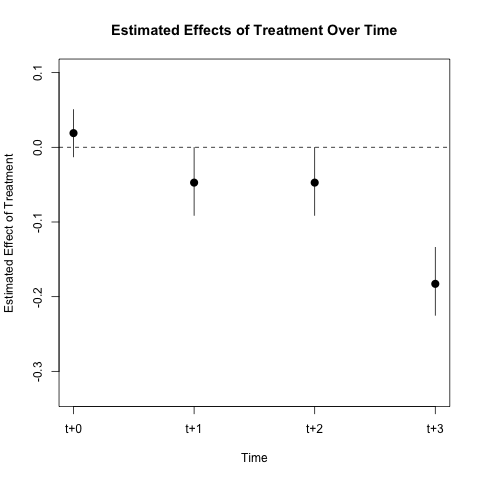
\includegraphics[width=0.9\textwidth]{Figures/acuerdo_gobestatal.png}
       \captionsetup{justification=centering}
       
        
 \textbf{Note:} Figure \ref{fig:matching} produced by propensity score matching that adjust for the treatment and covariate histories during the 5 year periods prior to the treatment. I report 95\% bootstrap confidence intervals clustered at the state level. Covariates include those used to generate Figure \ref{fig:event_study_agreements}. 

\end{figure}   
 
 \clearpage 
\begin{figure}[H] 
\centering
 \caption{Effect of Term Limit Reform on Security Cooperation Agreements signed with the Governor, 2010-2018}
 \label{fig:chaisemarting_agreements}
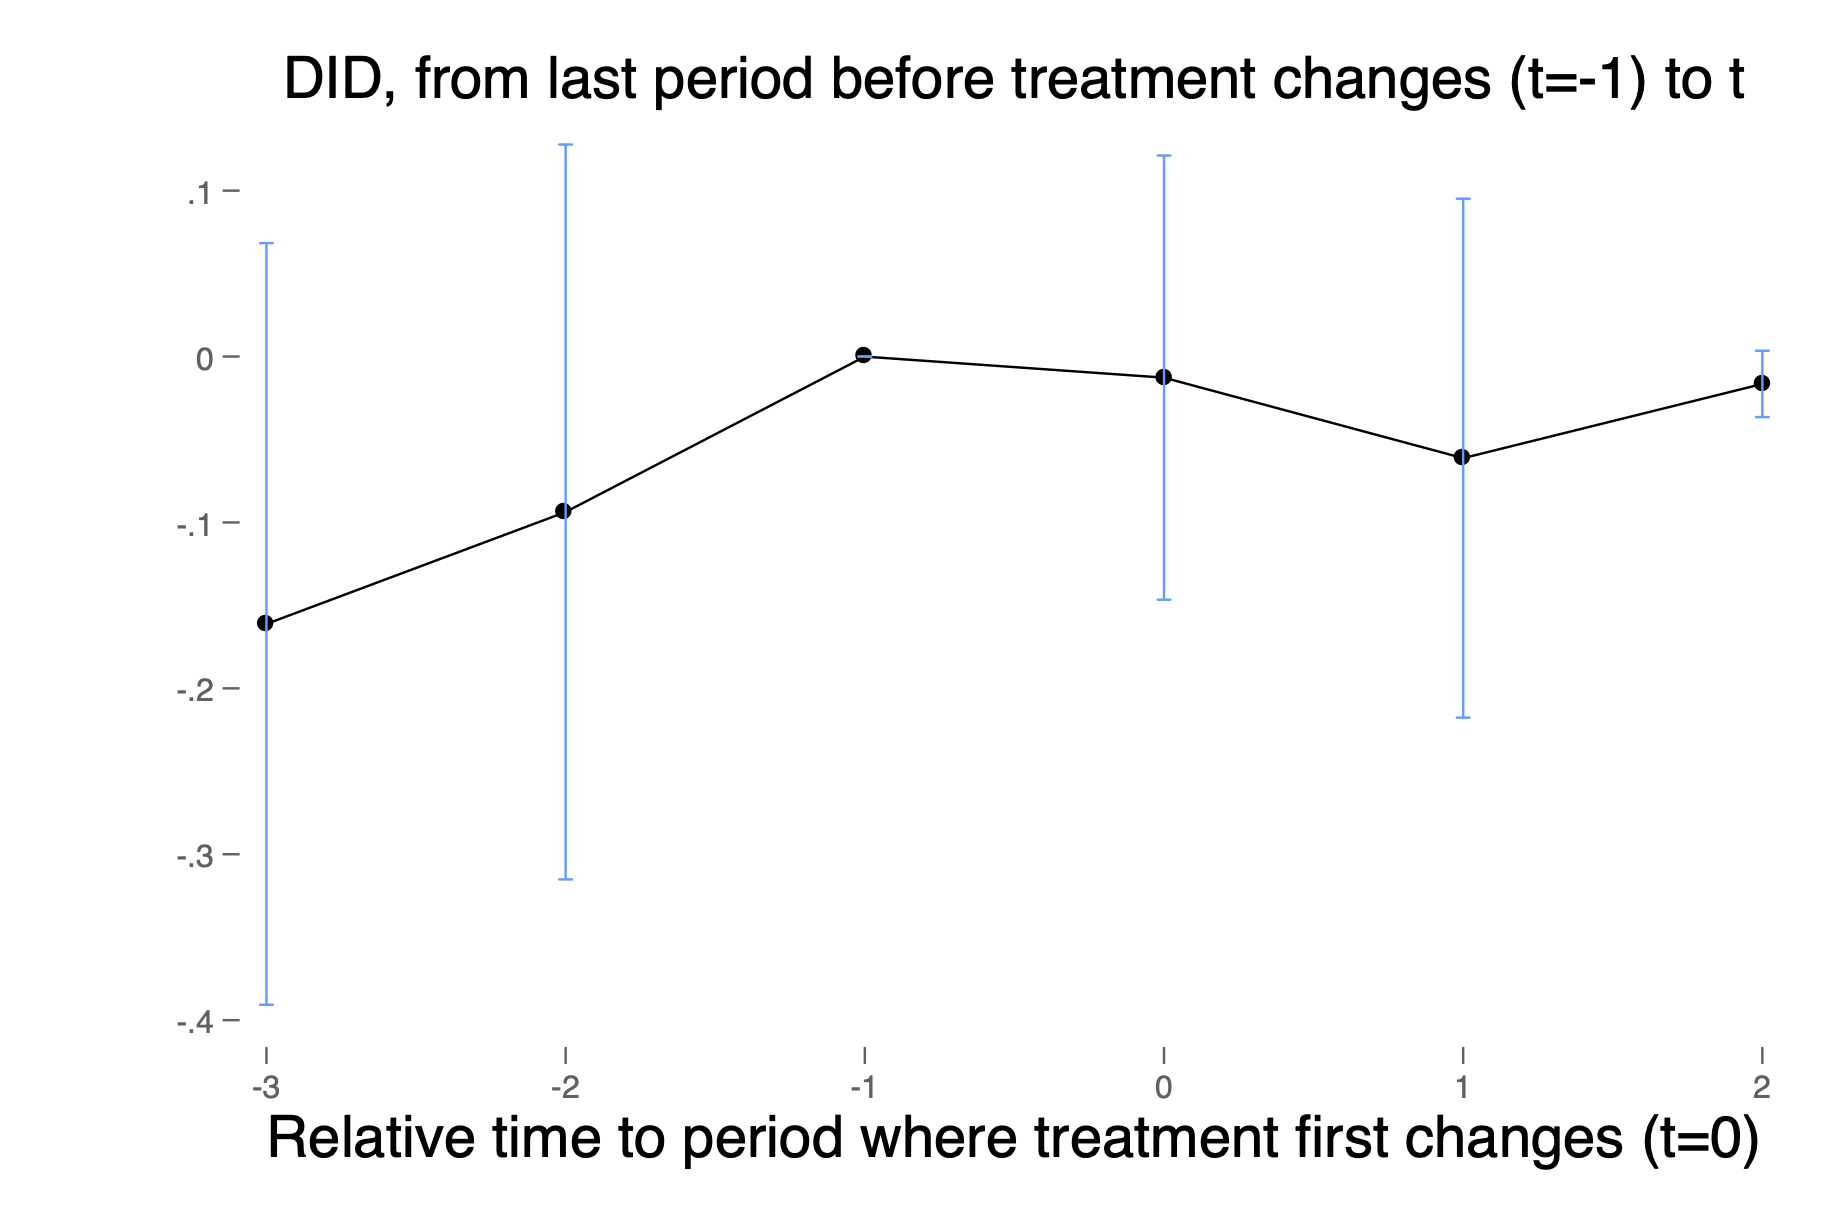
\includegraphics[width=0.9\textwidth]{Figures/chaisemartin_acuerdo_estcom.png}
       \captionsetup{justification=centering}
\end{figure}   

  %\begin{table}[htbp]\def\sym#1{\ifmmode^{#1}\else\(^{#1}\)\fi}
\centering
\caption{Comparison: Security Cooperation Agreements with Governor vs. Other Actors, 2014-2018}
\label{tab:as_comparison_agreements}
\scalebox{1}{
\begin{tabular}{lcc}
\hline \hline
\\ \multicolumn{3}{l}{Dependent variable: Security Cooperation Agreement}\\
& w/ Governor &  w/ Other Political Actors$^a$\\
& \multicolumn{1}{c}{(1)} & \multicolumn{1}{c}{(2)} \\
\cmidrule(lrr){2-2}  \cmidrule(lrr){3-3}\\
\addlinespace
Lag 4 years &         $ 0.0197^{} $ &      $ -0.0326^{} $  \\
& ($ 0.3292$) & ($ 0.0763 $) \\
Lag 3 years &        $ -0.0102^{***} $ &     $ 0.2193^{} $ \\
& ($ 0.0000$) & ($ 0.2702 $) \\
Lag 2 years &        $ 0.1418^{} $ &    $ -0.0648^{} $  \\
& ($ 0.1318$) & ($ 0.0524 $) \\
Reform, time 0 &        $ 0.0064^{} $ &     $ -0.0089^{} $ \\
& ($ 0.0354$) & ($ 0.0069 $) \\
Lead 1 year &         $ -0.2230^{***} $ &       $ -0.2858^{} $ \\
& ($ 0.0435$) & ($ 0.2610 $) \\
Lead 3 years &        $ -0.5921^{***} $ &     $ 0.1665^{} $ \\
& ($ 0.0708$) & ($ 0.1040 $) \\
\addlinespace
Observations       &                  4,382        &           4,382  \\
R-squared        &              0.6434        &           0.5469   \\
Mun. FEs       &     \checkmark         &  \checkmark    \\
Year. FEs       &     \checkmark         &  \checkmark   \\
Controls$^b$   &      \checkmark       &      \checkmark    \\
Cohort weighted   &   \checkmark       &   \checkmark    \\
WILD CI   &          &       \\
Aggregate effect        &              $-0.2696^{***} $$         &            $0.0796^{} $$   \\
SE (aggregate eff.)        &              (0.0339)       &           (0.0491)   \\
\hline \hline
\multicolumn{3}{p{0.7\textwidth}}{\footnotesize{Notes: Coefficients show IW estimators following \citet{abraham_sun_2020}. Two relative time periods (lag 5 and 1) are removed to avoid collinearity problems noted by \citet{abraham_sun_2020}. Standard errors in parentheses are clustered at the state level, with the following significance-level: $^{***}$ 1\%; $^{**}$ 5\%; and $^*$ 10\%, that refer to two-sided t-test with the null hypothesis equal to 0 for each relative time period. $^a$ Refers primarily to the President but could include Governors and mayors from other states or other municipalities from the same state. $^b$ Pretreatment controls include: governor winning margin; party alignment with the President;  party alignment with the Governor; municipal winning margin; logged population; logged organized crime related deaths; and Cartel presence.}} \\
\end{tabular}
}
\end{table}
   
  
  \begin{table}[htbp]\def\sym#1{\ifmmode^{#1}\else\(^{#1}\)\fi}
\centering
\caption{Effect of 2014 Term Limit Reform on the likelihood of signing Security Cooperation Agreements,  by type}
\label{tab:comparison_fed_estatal}
\scalebox{1}{
\begin{tabular}{lcccc}
\hline \hline
\\ \multicolumn{3}{l}{Dependent variable:}\\
& \multicolumn{2}{c}{Security Cooperation Agreement w/ Governor$^{a}$} & \multicolumn{2}{c}{Security Cooperation Agreement w/ Other$^{b}$} \\
& \multicolumn{1}{c}{(1)} & \multicolumn{1}{c}{(2)} & \multicolumn{1}{c}{(3)} & \multicolumn{1}{c}{(4)} \\
\cmidrule(lrr){2-3}  \cmidrule(lrr){4-5}\\
\addlinespace
t-4 &         $ 0.3497^{} $ &         $ 0.0193^{} $ &     $ -0.2763^{} $ &   $ -0.0326^{} $  \\
& ($ 1.8038$) & ($ 0.3316$) & ($ 0.5842$)  & ($ 0.0761 $) \\
t-3 &         $ -0.7355^{} $ &        $ -0.0102^{***} $  &     $ 0.2469^{} $ &     $ 0.2206^{} $ \\
& ($ 37.4159$) & ($ 0.0000$) & ($ 15.0281$) & ($ 0.2702 $) \\
t-2 &         $ 0.3861^{} $ &        $ 0.1420^{} $  &     $ -0.1496^{} $ &    $ -0.0649^{} $  \\
& ($ 0.3279$) & ($ 0.1323$) & ($ 0.1250$) & ($ 0.0524 $) \\
Reform (t=0) &         $ 0.2233^{***} $ &        $ 0.0065^{} $  &     $ -0.0599^{**} $  &     $ -0.0089^{} $ \\
& ($ 0.0581$) & ($ 0.0353$) & ($ 0.0273$) & ($ 0.0070 $) \\
t+1 &         $ -0.2198^{**} $ &         $ -0.2230^{***} $  &     $ 0.1148^{} $ &       $ -0.2845^{} $ \\
& ($ 0.0930$) & ($ 0.0435$) & ($ 0.0904$) & ($ 0.2602 $) \\
t+3 &         $ -0.5915^{***} $ &        $ -0.5921^{***} $ &     $ 0.1660^{*} $  &     $ 0.1665^{} $ \\
& ($ 0.0783$) & ($ 0.0708$) & ($ 0.0953$) & ($ 0.1040 $) \\
\addlinespace
Observations   &                  4,382     &                  4,382  &                  4,382        &           4,382  \\
R-squared      &              0.6433    &              0.6434   &            0.5469        &           0.5469   \\
Mun. FEs       &     \checkmark         &  \checkmark   &     \checkmark         &  \checkmark   \\
Year. FEs       &     \checkmark         &  \checkmark  &     \checkmark         &  \checkmark   \\
Controls$^b$   &      \checkmark       &      \checkmark   &      \checkmark       &      \checkmark   \\
Cohort weighted   &          &   \checkmark   &          &   \checkmark   \\
WILD CI  &     \checkmark         &  \checkmark   &     \checkmark         &  \checkmark   \\
Aggregate effect     &              $-0.213^{***} $$    &        $-0.2696^{***} $$      &            $0.069^{} $$   &       $0.0796^{} $$   \\
SE (aggregate eff.)      &              0.034   &              0.0339    &              0.045       &           0.0491   \\
\hline \hline
\multicolumn{5}{p{1.2\textwidth}}{\footnotesize{Notes: Coefficients in columns (2) and (4) show IW estimators following \citet{abraham_sun_2020}. In those models, two relative time periods (lag 8 and 1) are removed to avoid collinearity problems noted by \citet{abraham_sun_2020}. Standard errors in parentheses are clustered at the state level, with the following significance-level: $^{***}$ 1\%; $^{**}$ 5\%; and $^*$ 10\%, that refer to two-sided t-test with the null hypothesis equal to 0 for each relative time period. $^a$ Refers to security cooperation agreements signed with the governor only. $^b$ Refers to security cooperation agreements signed with other instituions but not the governor. $^c$ State-level controls include governor winning margin in last pre-treatment election and an indicator of whether the governor's party is the same as the federal incumbent party.}} \\
\end{tabular}
}
\end{table}
   
 
 
\def\sym#1{\ifmmode^{#1}\else\(^{#1}\)\fi}
\begin{table}[htbp]\def\sym#1{\ifmmode^{#1}\else\(^{#1}\)\fi}
\centering
\caption{Test on selection on unobservables}
\label{tab:unobservables}
\begin{tabular}{l*{1}{c}}
\hline \hline
&\multicolumn{1}{c}{(1)}         \\
\addlinespace
Fitted value&      0.1312         \\
            &    (0.0780)         \\
\addlinespace
Observations&      10,668         \\
R2          &       0.459         \\
Mun. FE     &      \checkmark               \\
Year FE     &      \checkmark               \\
State Cluster S.E.&     \checkmark                \\
\hline \hline 
\multicolumn{2}{p{0.6\textwidth}}{\footnotesize{Notes: I follow \citet{altonji_etal_2005} to check if unobserved variation is likely to explain the signing of security cooperation agreements with the Governor by mayors. To do so, I regress the treatment (whether the municipality held reelection) on all the available covariates used for Figure \ref{fig:event_study_agreements}.} I then take the fitted value from the regression and use it to predict each outcome, this time including unit and year fixed effects. This test suggests that – under the assumption that observables are representative of unobservables – selection on unobservables is not driving the results.} \\
\end{tabular}
\end{table} 

\clearpage 


\begin{comment}
\begin{figure}[H]
\centering
\caption{Effect of Electoral Reform on Security Cooperation Agreement using non parametric methods\\ -95\% confidence intervals-} 
\label{fig:non_did_agreement}
\begin{center} 
\begin{center} 
	{\textbf Figure A: Generalized Synthetic Control following \citet{xu_2016} }
\end{center}
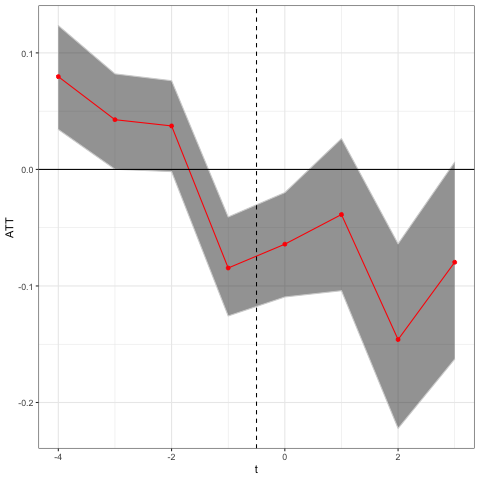
\includegraphics[width=0.55\textwidth]{Figures/gsynth_wcov_acuerdo.png}

\begin{center}
	{\textbf Figure B: Matrix Completion following \citet{Athey, Bayati, Doudchenko, Imbens, and Khosvari}
\end{center}
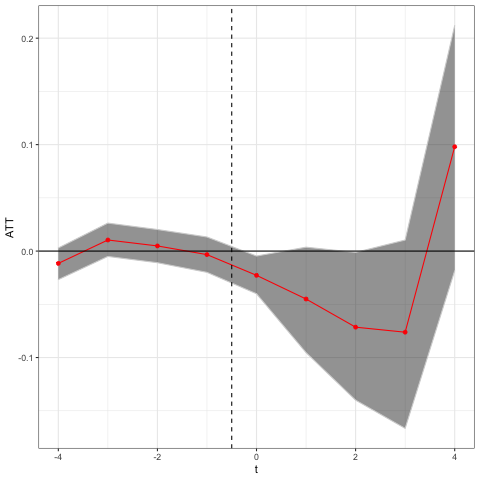
\includegraphics[width=0.55\textwidth]{Figures/matrix_completion.png}
       \captionsetup{justification=centering}
       \\
 %{\textbf Note: 95\% confidence intervals estimated using 1,000 bootstrap replications.} .   
\end{figure}      
\end{comment}


\clearpage

\subsection{Mechanisms}

\begin{figure}[H] 
\centering
 \caption{Effect of 2014 Term Limit Reform on Motives to Sign Security Agreements w/ Governor}
 \label{fig:motives}
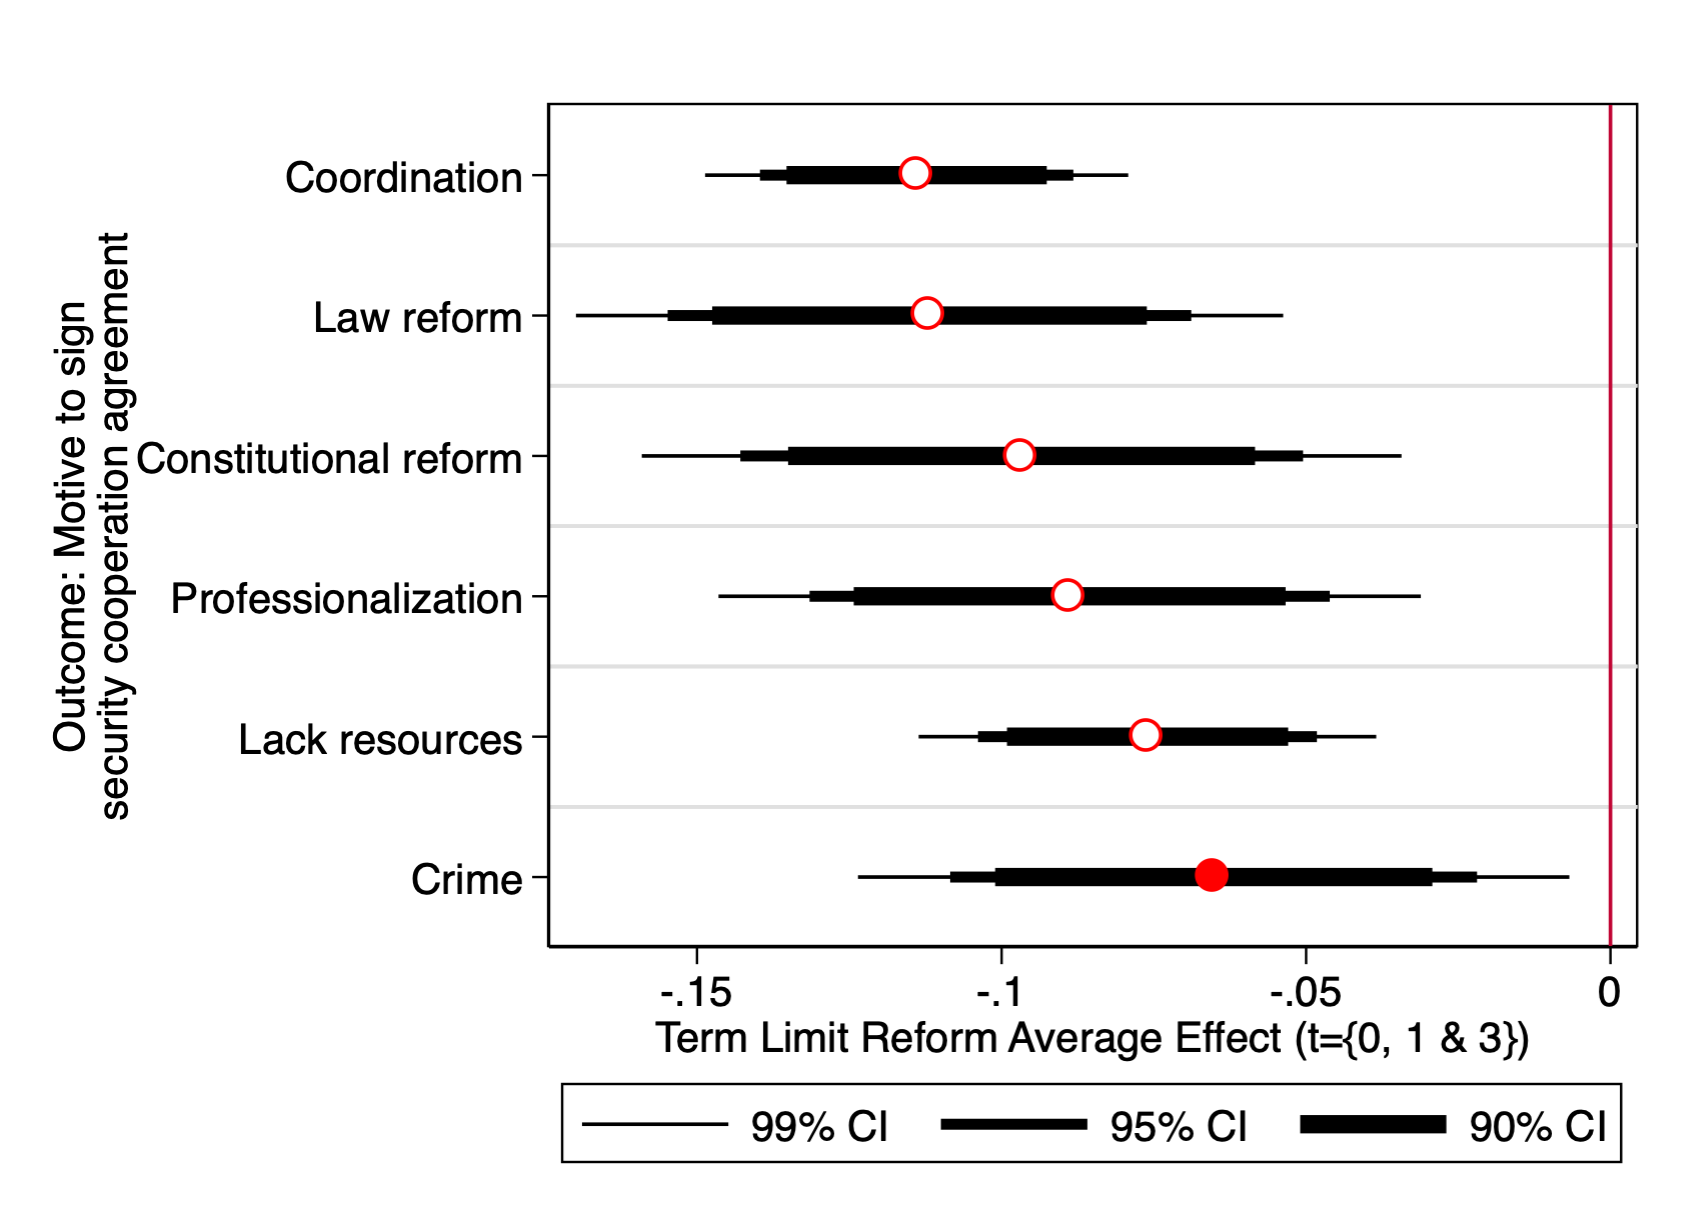
\includegraphics[width=0.9\textwidth]{Figures/motives.png}
       \captionsetup{justification=centering}
\end{figure}   

  \begin{landscape}
\begin{table}[htbp]\def\sym#1{\ifmmode^{#1}\else\(^{#1}\)\fi}
\centering
\caption{Effect of 2014 Term Limit Reform on Motives to Sign Security Agreements w/ Governor}
\label{tab:motives_final}
\scalebox{0.70}{
\begin{tabular}{lcccccc}
\hline \hline
\\ \multicolumn{7}{l}{Dependent variable:}\\
Motive: & Cons. reform  & Law reform & Lack resources & Professionalization & Coordination & Crime \\
& \multicolumn{1}{c}{(1)} & \multicolumn{1}{c}{(2)} & \multicolumn{1}{c}{(3)} & \multicolumn{1}{c}{(4)} & \multicolumn{1}{c}{(5)} & \multicolumn{1}{c}{(6)}  \\
\cmidrule(lrr){2-2}  \cmidrule(lrr){3-3} \cmidrule(lrr){4-4} \cmidrule(lrr){5-5} \cmidrule(lrr){6-6} \cmidrule(lrr){7-7} \\
\addlinespace
t-7 &     $ -0.2350^{***} $ &     $ -0.2581^{**} $ & $ -0.0955^{*} $ & $ -0.2000^{***} $  &     $ -0.1570^{*} $   &     $ -0.1538^{} $ \\
&     ($0.0407$) &     ($0.1175$) & ($0.0484$)& ($ 0.0671$)  &    ($0.0844$)   &   ($0.1078$) \\
t-6 &     $ -0.0758^{***} $ &     $ -0.0876^{***} $ &  $ -0.0615^{***} $ &  $ -0.0647^{} $  &     $ -0.0827^{**} $ &     $ -0.0369^{} $ \\
&     ($0.0176$) &     ($0.0199$) & ($0.0162$)& ($ 0.0585$)  &    ($0.0346$)   &   ($0.0265$) \\
t-5 &     $ 0.0223^{} $ &     $ -0.0405^{} $ &  $ 0.0574^{} $ &  $ 0.0580^{} $ &     $ -0.0106^{} $  &     $ 0.0427^{} $ \\
&     ($0.0591$) &     ($0.0583$) & ($0.0481$)& ($ 0.0750$)  &    ($0.0709$)   &   ($0.0445$) \\
t-4 &     $ 0.0167^{} $ &     $ -0.0832^{} $ &   $ 0.1207^{} $ &   $ 0.0649^{} $  &     $ -0.1313^{} $ &     $ 0.0346^{} $ \\
&     ($0.0987$) &     ($0.0842$) & ($0.0854$)& ($ 0.1053$)  &    ($0.2085$)   &   ($0.1173$) \\
t-3 &     $ -0.0385^{} $ &     $ -0.0160^{} $ &   $ 0.0727^{} $ &   $ 0.0802^{} $  &     $ 0.0403^{} $ &     $ 0.0734^{} $ \\
&     ($0.1052$) &     ($0.0840$) & ($0.1002$)& ($ 0.0738$)  &    ($0.1662$)   &   ($0.1061$) \\
t-2 &     $ -0.1162^{} $ &     $ -0.0914^{} $ &  $ 0.0228^{} $  &  $ -0.0822^{} $  &     $ -0.2796^{*} $ &     $ -0.0753^{} $ \\
&     ($0.1012$) &     ($0.0917$) & ($0.0640$)& ($ 0.1195$)  &    ($0.1379$)   &   ($0.0667$) \\
Reform (t=0) &     $ 0.0457^{} $ &     $ 0.0292^{} $ &   $ 0.0214^{} $   &   $ 0.0282^{} $  &     $ 0.0233^{} $ &     $ 0.0272^{*} $ \\
&     ($0.0278$) &     ($0.0183$) & ($0.0179$)& ($ 0.0201$)  &    ($0.0209$)   &   ($0.0146$) \\
t+1 &     $ -0.0906^{***} $ &     $ -0.1071^{***} $ &    $ -0.0935^{***} $ &    $ -0.0935^{***} $ &     $ -0.1215^{***} $ &     $ -0.0735^{***} $  \\
&     ($0.0164$) &     ($0.0182$) & ($0.0106$)& ($ 0.0160$)  &    ($0.0291$)   &   ($0.0121$) \\
t+3 &     $ -0.2452^{***} $ &     $ -0.2576^{***} $ &   $ -0.1560^{***} $  &   $ -0.2011^{***} $ &     $ -0.2436^{***} $ &     $ -0.1492^{***} $ \\
&     ($0.0535$) &     ($0.0484$) & ($0.0350$)& ($ 0.0463$)  &    ($0.0431$)   &   ($0.0527$) \\
\\
\addlinespace
Observations       &              9,725    &              9,725    &           9,725      &           9,725  &              9,725    &              9,725     \\
R-squared        &          0.2974 &          0.3021    &    0.2617       &           0.2722 &          0.2865 &          0.2594      \\
Mun. FEs      &     \checkmark         &  \checkmark   &     \checkmark         &  \checkmark  &     \checkmark         &  \checkmark   &     \checkmark         &  \checkmark   \\
Year. FEs    &     \checkmark         &  \checkmark   &     \checkmark         &  \checkmark &     \checkmark         &  \checkmark   &     \checkmark         &  \checkmark   \\
Controls$^b$  &    \checkmark     &       \checkmark  &    \checkmark      &   \checkmark &    \checkmark     &       \checkmark  &    \checkmark      &   \checkmark     \\
Cohort weighted  &   \checkmark      &       \checkmark  &   \checkmark       &   \checkmark  &   \checkmark      &       \checkmark  &   \checkmark       &   \checkmark    \\
Reform aggregate effect         & $-0.0967^{***} $$      & $-0.1118^{***} $$    & $-0.0760^{***} $$      & $-0.0888^{***} $$     & $-0.1139^{***} $$      & $-0.0652^{***} $$     \\
SE       & (0.0225)  & (0.0210) & (0.0136)  & (0.0208)  & (0.0125)  & (0.0211)   \\
\hline \hline
\multicolumn{7}{p{1.2\textwidth}}{\footnotesize{Notes: Coefficients show IW estimators following \citet{abraham_sun_2020}. Two relative time periods (lag 8 and 1) are removed to avoid collinearity problems noted by \citet{abraham_sun_2020}. Standard errors in parentheses are clustered at the state level for estimates in saturaded model. Significance-level: $^{***}$ 1\%; $^{**}$ 5\%; and $^*$ 10\%, that refer to two-sided t-test with the null hypothesis equal to 0 for each relative time period. $^a$ Even columns with outcomes with missing values where replaced by zeros assuming no activity was registered. $^b$ State-level controls include governor winning margin in last pre-treatment election and an indicator of whether the governor's party is the same as the federal incumbent party.}} \\
\end{tabular}
}
\end{table}
\end{landscape}
   

   %\begin{landscape}
\begin{table}[htbp]\def\sym#1{\ifmmode^{#1}\else\(^{#1}\)\fi}
\centering
\caption{Effect of 2014 Term Limit Reform on Motives to Sign Security Agreements w/ Governor}
\label{tab:motives_average_final}
\scalebox{0.70}{
\begin{tabular}{lcccccc}
\hline \hline
\\ \multicolumn{7}{l}{Dependent variable:}\\
Motive: & Cons. reform  & Law reform & Lack resources & Professionalization & Coordination & Crime \\
& \multicolumn{1}{c}{(1)} & \multicolumn{1}{c}{(2)} & \multicolumn{1}{c}{(3)} & \multicolumn{1}{c}{(4)} & \multicolumn{1}{c}{(5)} & \multicolumn{1}{c}{(6)}  \\
\cmidrule(lrr){2-2}  \cmidrule(lrr){3-3} \cmidrule(lrr){4-4} \cmidrule(lrr){5-5} \cmidrule(lrr){6-6} \cmidrule(lrr){7-7} \\
\addlinespace
Reform average effect         & $-0.0967^{***} $$      & $-0.1118^{***} $$     & $-0.0760^{***} $$        & $-0.0888^{***} $$       & $-0.1139^{***} $$        & $-0.0652^{***} $$       \\
& (0.0225)  & (0.0210) & (0.0136)  & (0.0208)  & (0.0125)  & (0.0211)   \\
\\
\addlinespace
Observations       &              9,725    &              9,725    &           9,725      &           9,725  &              9,725    &              9,725    \\
R-squared        &          0.2974 &          0.3021    &    0.2617       &           0.2722 &          0.2865 &          0.2594   \\
Mun. FEs      &     \checkmark         &  \checkmark   &     \checkmark         &  \checkmark  &     \checkmark         &  \checkmark   &     \checkmark         &  \checkmark   \\
Year. FEs    &     \checkmark         &  \checkmark   &     \checkmark         &  \checkmark &     \checkmark         &  \checkmark   &     \checkmark         &  \checkmark   \\
Controls$^b$  &    \checkmark     &       \checkmark  &    \checkmark      &   \checkmark &    \checkmark     &       \checkmark  &    \checkmark      &   \checkmark     \\
Cohort weighted  &   \checkmark      &       \checkmark  &   \checkmark       &   \checkmark  &   \checkmark      &       \checkmark  &   \checkmark       &   \checkmark    \\
Parallel trend holds &   \checkmark      &       \checkmark  &   \checkmark       &   \checkmark  &   \checkmark      &       \checkmark  &   \checkmark       &   \checkmark    \\
\hline \hline
\multicolumn{7}{p{1.2\textwidth}}{\footnotesize{Notes: Coefficients show IW estimators following \citet{abraham_sun_2020}. Two relative time periods (lag 8 and 1) are removed to avoid collinearity problems noted by \citet{abraham_sun_2020}. Standard errors in parentheses are clustered at the state level for estimates in saturaded model. Significance-level: $^{***}$ 1\%; $^{**}$ 5\%; and $^*$ 10\%, that refer to two-sided t-test with the null hypothesis equal to 0 for each relative time period. $^a$ Even columns with outcomes with missing values where replaced by zeros assuming no activity was registered. $^b$ State-level controls include governor winning margin in last pre-treatment election and an indicator of whether the governor's party is the same as the federal incumbent party.}} \\
\end{tabular}
}
\end{table}
\end{landscape}
  
   
   
      
\begin{landscape}
\begin{table}[htbp]\def\sym#1{\ifmmode^{#1}\else\(^{#1}\)\fi}
\centering
\caption{Effect of 2014 Term Limit Reform on Services Delegated to the Governor}
\label{tab:services}
\scalebox{0.70}{
\begin{tabular}{lcccccccc}
\hline \hline
\\ \multicolumn{9}{l}{Dependent variable:}\\
Service delegated: & Public security  & Traffic & Prevention & Training  & Technology & Research & Inteligence & Unify procedures \\
& \multicolumn{1}{c}{(1)} & \multicolumn{1}{c}{(2)} & \multicolumn{1}{c}{(3)} & \multicolumn{1}{c}{(4)} & \multicolumn{1}{c}{(5)} & \multicolumn{1}{c}{(6)} & \multicolumn{1}{c}{(7)} & \multicolumn{1}{c}{(8)} \\
\cmidrule(lrr){2-2}  \cmidrule(lrr){3-3} \cmidrule(lrr){4-4} \cmidrule(lrr){5-5} \cmidrule(lrr){6-6} \cmidrule(lrr){7-7} \cmidrule(lrr){8-8} \cmidrule(lrr){9-9} \\
\addlinespace
t-2 &     $ -0.0244^{} $ &     $ -0.0441^{} $ &  $ -0.0598^{***} $  &  $ -0.0565^{***} $  &     $ -0.0567^{***} $ &     $ -0.0596^{***} $ & $ -0.0596^{***} $ & $ -0.0506^{***} $   \\
&     ($0.1046$) &     ($0.0818$) & ($0.0021$)& ($ 0.0012$)  &    ($0.0016$)   &   ($0.0017$) \\
Reform (t=0) &     $ 0.0702^{} $ &     $ 0.0256^{} $ &   $ 0.0175^{} $   &   $ 0.0214^{} $  &     $ 0.0194^{} $ &     $ 0.0194^{} $ & $ 0.0204^{} $ & $ 0.0233^{} $   \\
&     ($0.0436$) &     ($0.0369$) & ($0.0137$)& ($ 0.0142$)  &    ($0.0126$)   &   ($0.0138$) \\
t+1 &     $ -0.0947^{*} $ &     $ -0.0259^{*} $ &    $ 0.0106^{} $ &    $ 0.0053^{} $ &     $ 0.0047^{} $ &     $ 0.0024^{} $  & $ 0.0018^{} $ & $ 0.0053^{} $   \\
&     ($0.0509$) &     ($0.0147$) & ($0.0198$)& ($ 0.0193$)  &    ($0.0197$)   &   ($0.0201$) \\
t+3 &     $ -0.2847^{***} $ &     $ 0.0000^{} $  \\
&     ($0.0430$) &     ($0.0000$)  \\
\\
\addlinespace
Observations       &              4,865    &              4,865    &           3,244      &           3,244  &              3,244    &              3,244  &              3,244    &              6,481   \\
R-squared        &          0.4234 &          0.3703    &    0.5567       &           0.5477 &          0.5409 &          0.5473     &        0.5467    &        0.4894   \\
Mun. FEs      &     \checkmark         &  \checkmark   &     \checkmark         &  \checkmark  &     \checkmark         &  \checkmark   &     \checkmark         &  \checkmark   \\
Year. FEs    &     \checkmark         &  \checkmark   &     \checkmark         &  \checkmark &     \checkmark         &  \checkmark   &     \checkmark         &  \checkmark   \\
Controls$^b$  &    \checkmark     &       \checkmark  &    \checkmark      &   \checkmark &    \checkmark     &       \checkmark  &    \checkmark      &   \checkmark     \\
Cohort weighted  &   \checkmark      &       \checkmark  &   \checkmark       &   \checkmark  &   \checkmark      &       \checkmark  &   \checkmark       &   \checkmark    \\
Reform average effect         & $-0.1031^{***} $$      & $-0.0242^{} $$     & $0.0094^{} $$        & $0.0133^{} $$       & $0.0121^{} $$        & $0.0109^{} $$    & $0.0111^{} $$      & $0.0143^{} $$     \\
SE (average effect)      & (0.0225)  & (0.0162) & (0.0080)  & (0.0120)  & (0.0117)  & (0.0122)    & (0.0123)  & (0.0114)   \\
\hline \hline
\multicolumn{9}{p{1.5\textwidth}}{\footnotesize{Notes: Coefficients show IW estimators following \citet{abraham_sun_2020}. Two relative time periods (lag 8 and 1) are removed to avoid collinearity problems noted by \citet{abraham_sun_2020}. Standard errors in parentheses are clustered at the state level for estimates in saturaded model. Significance-level: $^{***}$ 1\%; $^{**}$ 5\%; and $^*$ 10\%, that refer to two-sided t-test with the null hypothesis equal to 0 for each relative time period. $^a$ Even columns with outcomes with missing values where replaced by zeros assuming no activity was registered. $^b$ State-level controls include governor winning margin in last pre-treatment election and an indicator of whether the governor's party is the same as the federal incumbent party.}} \\
\end{tabular}
}
\end{table}
\end{landscape}
   
%\begin{landscape}
\begin{table}[htbp]\def\sym#1{\ifmmode^{#1}\else\(^{#1}\)\fi}
\centering
\caption{Effect of 2014 Term Limit Reform on Services Delegated to the Governor}
\label{tab:services_average}
\scalebox{0.70}{
\begin{tabular}{lcccccccc}
\hline \hline
\\ \multicolumn{9}{l}{Dependent variable:}\\
Service delegated: & Public security  & Traffic & Prevention & Training  & Technology & Research & Inteligence & Unify procedures \\
& \multicolumn{1}{c}{(1)} & \multicolumn{1}{c}{(2)} & \multicolumn{1}{c}{(3)} & \multicolumn{1}{c}{(4)} & \multicolumn{1}{c}{(5)} & \multicolumn{1}{c}{(6)} & \multicolumn{1}{c}{(7)} & \multicolumn{1}{c}{(8)} \\
\cmidrule(lrr){2-2}  \cmidrule(lrr){3-3} \cmidrule(lrr){4-4} \cmidrule(lrr){5-5} \cmidrule(lrr){6-6} \cmidrule(lrr){7-7} \cmidrule(lrr){8-8} \cmidrule(lrr){9-9} \\
\addlinespace
Reform average effect         & $0.0149^{*} $$      & $0.0579^{***} $$     & $0.0426^{***} $$        & $0.0034^{} $$       & $-0.0345^{***} $$        & $-0.0819^{***} $$    & $0.0092^{} $$      & $0.0056^{} $$     \\
SE       & (0.0079)  & (0.0099) & (0.0046)  & (0.0048)  & (0.0103)  & (0.0085)    & (0.0063)  & (0.0034)   \\
\addlinespace
Observations       &             11,353    &             11,353    &          11,353      &          11,353  &             11,353    &             11,353  &             11,353    &             11,353   \\
R-squared        &          0.8662 &          0.8556    &    0.9239       &           0.8767 &          0.8548 &          0.8954     &        0.8557    &        0.7008   \\
Mun. FEs      &     \checkmark         &  \checkmark   &     \checkmark         &  \checkmark  &     \checkmark         &  \checkmark   &     \checkmark         &  \checkmark   \\
Year. FEs    &     \checkmark         &  \checkmark   &     \checkmark         &  \checkmark &     \checkmark         &  \checkmark   &     \checkmark         &  \checkmark   \\
Controls$^b$  &    \checkmark     &       \checkmark  &    \checkmark      &   \checkmark &    \checkmark     &       \checkmark  &    \checkmark      &   \checkmark     \\
Cohort weighted  &   \checkmark      &       \checkmark  &   \checkmark       &   \checkmark  &   \checkmark      &       \checkmark  &   \checkmark       &   \checkmark    \\
Parallel trend holds &   \checkmark      &       \checkmark  &          &     &         &       &          &       \\
\hline \hline
\multicolumn{9}{p{1.5\textwidth}}{\footnotesize{Notes: Coefficients show IW estimators following \citet{abraham_sun_2020}. Two relative time periods (lag 8 and 1) are removed to avoid collinearity problems noted by \citet{abraham_sun_2020}. Standard errors in parentheses are clustered at the state level for estimates in saturaded model. Significance-level: $^{***}$ 1\%; $^{**}$ 5\%; and $^*$ 10\%, that refer to two-sided t-test with the null hypothesis equal to 0 for each relative time period. $^a$ Even columns with outcomes with missing values where replaced by zeros assuming no activity was registered. $^b$ State-level controls include governor winning margin in last pre-treatment election and an indicator of whether the governor's party is the same as the federal incumbent party.}} \\
\end{tabular}
}
\end{table}
\end{landscape}
   

\begin{landscape}
\begin{table}[htbp]\def\sym#1{\ifmmode^{#1}\else\(^{#1}\)\fi}
\centering
\caption{Effect of 2014 Term Limit Reform on Services Delegated to the Governor}
\label{tab:interaction_alignment}
\scalebox{0.70}{
\begin{tabular}{lccc}
\hline \hline
\\ \multicolumn{4}{l}{Dependent variable: Signing Security Cooperation Agreement w/ Governor}\\
Alignment: & w/ President  & w/ Governor  & w/ Governor from PRI \\
& \multicolumn{1}{c}{(1)} & \multicolumn{1}{c}{(2)} & \multicolumn{1}{c}{(3)} \\
\cmidrule(lrr){2-2}  \cmidrule(lrr){3-3} \cmidrule(lrr){4-4} \\
\addlinespace
t-7 &     $ -0.2383^{*} $ &     $ -0.0191^{*} $ &  $ 0.0000^{} $ \\
&     ($0.1348$) &     ($0.0108$) & ($0.0000$) \\
t-6 &     $ -0.0807^{} $ &     $ 0.0199^{} $ &  $ -0.0430^{} $  \\
&     ($0.0873$) &     ($0.0499$) & ($0.0467$) \\
t-5 &     $ -0.1186^{} $ &     $ -0.2028^{**} $ &  $ -0.2406^{**} $  \\
&     ($0.1046$) &     ($0.0924$) & ($0.0922$) \\
t-4 &     $ 0.0665^{} $ &     $ -0.0784^{} $ &  $ -0.1077^{} $  \\
&     ($0.1483$) &     ($0.1203$) & ($0.1236$) \\
t-3 &     $ 0.3395^{**} $ &     $ 0.2569^{***} $ &  $ 0.2303^{***} $  \\
&     ($0.1651$) &     ($0.0720$) & ($0.0702$) \\
t-2 &     $ 0.0027^{} $ &     $ -0.0253^{} $ &  $ 0.0976^{} $  \\
&     ($0.1572$) &     ($0.1182$) & ($0.1471$) \\
Reform (t=0) &     $ -0.1686^{} $ &     $ -0.2236^{} $ &   $ 0.1790^{} $   \\
&     ($0.1877$) &     ($0.1316$) & ($0.1258$) \\
t+1 &     $ -0.2169^{} $ &     $ -0.5692^{**} $ &    $ -0.0199^{} $ \\
&     ($0.1884$) &     ($0.2119$) & ($0.1549$) \\
t+2 &     $ -0.1125^{} $ &     $ -0.5020^{*} $  &     $ -0.4753^{*} $ \\
&     ($0.2496$) &     ($0.2690$)  & ($0.2741$) \\
t+3 &     $ -0.2197^{} $ &     $ -0.3562^{} $  &     $ -0.3876^{} $ \\
&     ($0.2241$) &     ($0.3827$)  & ($0.3818$) \\
\\
\addlinespace
Observations       &             12,173    &             12,173    &          12,173    \\
R-squared        &          0.4555 &          0.4566    &    0.4541    \\
Mun. FEs      &     \checkmark         &  \checkmark   &     \checkmark    \\
Year. FEs    &     \checkmark         &  \checkmark   &     \checkmark    \\
Controls$^b$  &    \checkmark     &       \checkmark  &    \checkmark   \\
Cohort weighted  &   \checkmark      &       \checkmark  &   \checkmark    \\
Reform average effect         & $-0.1376^{} $$      & $-0.1538^{*} $$     & $-0.0551^{} $$     \\
SE (average effect)      & (0.1313)  & (0.0906) & (0.0652) \\
\hline \hline
\multicolumn{4}{p{1.5\textwidth}}{\footnotesize{Notes: Coefficients show IW estimators following \citet{abraham_sun_2020}. Two relative time periods (lag 8 and 1) are removed to avoid collinearity problems noted by \citet{abraham_sun_2020}. Standard errors in parentheses are clustered at the state level for estimates in saturaded model. Significance-level: $^{***}$ 1\%; $^{**}$ 5\%; and $^*$ 10\%, that refer to two-sided t-test with the null hypothesis equal to 0 for each relative time period. $^a$ Even columns with outcomes with missing values where replaced by zeros assuming no activity was registered. $^b$ State-level controls include governor winning margin in last pre-treatment election and an indicator of whether the governor's party is the same as the federal incumbent party.}} \\
\end{tabular}
}
\end{table}
\end{landscape}
   
%\begin{landscape}
\begin{table}[htbp]\def\sym#1{\ifmmode^{#1}\else\(^{#1}\)\fi}
\centering
\caption{Effect of 2014 Term Limit Reform on Services Delegated to the Governor}
\label{tab:interaction_alignment_average}
\scalebox{0.70}{
\begin{tabular}{lccc}
\hline \hline
\\ \multicolumn{4}{l}{Dependent variable: Signing Security Cooperation Agreement w/ Governor}\\
Alignment: & w/ President  & w/ Governor  & w/ Governor from PRI \\
& \multicolumn{1}{c}{(1)} & \multicolumn{1}{c}{(2)} & \multicolumn{1}{c}{(3)} \\
\cmidrule(lrr){2-2}  \cmidrule(lrr){3-3} \cmidrule(lrr){4-4} \\
\addlinespace
Reform average effect         & $-0.1376^{} $$      & $-0.1538^{*} $$     & $-0.0551^{} $$     \\
& (0.1313)  & (0.0906) & (0.0652) \\
\\
\addlinespace
Observations       &             12,173    &             12,173    &          12,173    \\
R-squared        &          0.4555 &          0.4566    &    0.4541    \\
Mun. FEs      &     \checkmark         &  \checkmark   &     \checkmark    \\
Year. FEs    &     \checkmark         &  \checkmark   &     \checkmark    \\
Controls$^b$  &    \checkmark     &       \checkmark  &    \checkmark   \\
Cohort weighted  &   \checkmark      &       \checkmark  &   \checkmark    \\
\hline \hline
\multicolumn{4}{p{1.5\textwidth}}{\footnotesize{Notes: Coefficients show IW estimators following \citet{abraham_sun_2020}. Two relative time periods (lag 8 and 1) are removed to avoid collinearity problems noted by \citet{abraham_sun_2020}. Standard errors in parentheses are clustered at the state level for estimates in saturaded model. Significance-level: $^{***}$ 1\%; $^{**}$ 5\%; and $^*$ 10\%, that refer to two-sided t-test with the null hypothesis equal to 0 for each relative time period. $^a$ Even columns with outcomes with missing values where replaced by zeros assuming no activity was registered. $^b$ State-level controls include governor winning margin in last pre-treatment election and an indicator of whether the governor's party is the same as the federal incumbent party.}} \\
\end{tabular}
}
\end{table}
\end{landscape}
   

        
\begin{landscape}
\begin{table}[htbp]\def\sym#1{\ifmmode^{#1}\else\(^{#1}\)\fi}
\centering
\caption{Effect of 2014 Term Limit Reform on Services Delegated to the Governor}
\label{tab:interaction_trust}
\scalebox{0.70}{
\begin{tabular}{lcccccccc}
\hline \hline
\\ \multicolumn{9}{l}{Dependent variable: Signing Security Cooperation Agreement w/ Governor}\\
Jurisdiction: & \multicolumn{2}{c}{Municipal} & \multicolumn{2}{c}{State} & \multicolumn{4}{c}{Federal} \\
Police force: & Traffic  & Preventive  & State Police & State Attorney Police & Federal Police & Ministerial Police & Army & Marines \\
& \multicolumn{1}{c}{(1)} & \multicolumn{1}{c}{(2)} & \multicolumn{1}{c}{(3)} & \multicolumn{1}{c}{(4)} & \multicolumn{1}{c}{(5)} & \multicolumn{1}{c}{(6)} & \multicolumn{1}{c}{(7)} & \multicolumn{1}{c}{(8)} \\
\cmidrule(lrr){2-2}  \cmidrule(lrr){3-3} \cmidrule(lrr){4-4} \cmidrule(lrr){5-5} \cmidrule(lrr){6-6} \cmidrule(lrr){7-7} \cmidrule(lrr){8-8} \cmidrule(lrr){9-9} \\
\addlinespace
t-7 &     $ 0.1781^{} $ &     $ 0.0000^{} $ &  $ 0.1737^{} $  &  $ 0.1270^{} $  &     $ 0.0908^{} $ &     $ 0.1162^{} $ & $ 0.1093^{*} $ & $ 0.0788^{} $   \\
&     ($0.1657$) &     ($0.0000$) & ($0.1372$)& ($ 0.1137$)  &    ($0.0736$)   &   ($0.0858$) \\
t-6 &     $ -0.0459^{} $ &     $ -0.0601^{} $ &  $ -0.0414^{} $  &  $ -0.0565^{} $  &     $ 0.0055^{} $ &     $ -0.0537^{} $ & $ 0.0234^{} $ & $ 0.0038^{} $   \\
&     ($0.0801$) &     ($0.0481$) & ($0.0539$)& ($ 0.0457$)  &    ($0.0390$)   &   ($0.0379$) \\
t-5 &     $ -0.8924^{***} $ &     $ -0.2958^{} $ &  $ -0.7754^{} $  &  $ -1.3246^{} $  &     $ -0.8583^{**} $ &     $ -1.3844^{***} $ & $ -0.6699^{**} $ & $ -0.5789^{} $   \\
&     ($0.2538$) &     ($0.2470$) & ($0.6291$)& ($ 0.9127$)  &    ($0.3310$)   &   ($0.2853$) \\
t-4 &     $ -0.8387^{} $ &     $ -0.4847^{} $ &  $ -0.8341^{} $  &  $ -1.8134^{} $  &     $ -1.0918^{} $ &     $ -1.2394^{} $ & $ -0.3796^{} $ & $ -0.4926^{} $   \\
&     ($0.7688$) &     ($0.7827$) & ($0.7594$)& ($ 1.3210$)  &    ($0.7492$)   &   ($1.0419$) \\
t-3 &     $ -0.0581^{} $ &     $ -0.2251^{} $ &  $ -0.4852^{} $  &  $ -1.8471^{} $  &     $ -0.6960^{} $ &     $ -0.8290^{} $ & $ 0.1192^{} $ & $ -0.1124^{} $   \\
&     ($0.8135$) &     ($0.8597$) & ($0.7511$)& ($ 1.3390$)  &    ($0.8562$)   &   ($1.1144$) \\
t-2 &     $ 0.0341^{} $ &     $ -0.2671^{} $ &  $ -0.2891^{} $  &  $ -0.6196^{} $  &     $ -0.6138^{} $ &     $ -0.3468^{} $ & $ -0.4246^{} $ & $ -0.4023^{} $   \\
&     ($0.5384$) &     ($0.5922$) & ($0.4176$)& ($ 0.8966$)  &    ($0.4795$)   &   ($0.7851$) \\
Reform (t=0) &     $ -0.4444^{} $ &     $ 0.1161^{} $ &   $ -0.5432^{} $   &   $ -0.3590^{} $  &     $ -1.2942^{**} $ &     $ -0.8581^{} $ & $ -0.4514^{} $ & $ -0.8446^{} $   \\
&     ($0.4490$) &     ($0.4975$) & ($0.4116$)& ($ 1.1629$)  &    ($0.5674$)   &   ($0.7678$) \\
t+1 &     $ -0.9836^{} $ &     $ -0.2186^{} $ &    $ -1.3877^{**} $ &    $ -1.3449^{} $ &     $ -2.4941^{***} $ &     $ -1.8551^{*} $  & $ -1.5407^{**} $ & $ -1.8918^{**} $   \\
&     ($0.5947$) &     ($0.5769$) & ($0.6053$)& ($ 1.4393$)  &    ($0.7475$)   &   ($0.9449$) \\
t+2 &     $ -1.8506^{***} $ &     $ -1.6311^{**} $  \\
&     ($0.5938$) &     ($0.6871$)  \\
t+3 &     $ -0.1376^{} $ &     $ -1.5275^{} $  \\
&     ($1.1164$) &     ($1.1456$)  \\
\\
\addlinespace
Observations       &             12,173    &             12,173    &          12,173      &          12,173  &             12,173    &             12,173  &             12,173    &             12,173   \\
R-squared        &          0.4666 &          0.4641    &    0.4675       &           0.4673 &          0.4642 &          0.4719     &        0.4666    &        0.4666   \\
Mun. FEs      &     \checkmark         &  \checkmark   &     \checkmark         &  \checkmark  &     \checkmark         &  \checkmark   &     \checkmark         &  \checkmark   \\
Year. FEs    &     \checkmark         &  \checkmark   &     \checkmark         &  \checkmark &     \checkmark         &  \checkmark   &     \checkmark         &  \checkmark   \\
Controls$^b$  &    \checkmark     &       \checkmark  &    \checkmark      &   \checkmark &    \checkmark     &       \checkmark  &    \checkmark      &   \checkmark     \\
Cohort weighted  &   \checkmark      &       \checkmark  &   \checkmark       &   \checkmark  &   \checkmark      &       \checkmark  &   \checkmark       &   \checkmark    \\
Reform average effect         & $-0.1399^{} $$      & $-0.2053^{} $$     & $-0.3431^{**} $$        & $-0.2984^{**} $$       & $-0.5738^{**} $$        & $-0.2614^{**} $$    & $-0.4633^{} $$      & $-0.4835^{*} $$     \\
SE (average effect)      & (0.0944)  & (0.1633) & (0.1594)  & (0.1455)  & (0.2673)  & (0.1107)    & (0.4247)  & (0.2373)   \\
\hline \hline
\multicolumn{9}{p{1.5\textwidth}}{\footnotesize{Notes: Coefficients show IW estimators following \citet{abraham_sun_2020}. Two relative time periods (lag 8 and 1) are removed to avoid collinearity problems noted by \citet{abraham_sun_2020}. Standard errors in parentheses are clustered at the state level for estimates in saturaded model. Significance-level: $^{***}$ 1\%; $^{**}$ 5\%; and $^*$ 10\%, that refer to two-sided t-test with the null hypothesis equal to 0 for each relative time period. $^a$ Even columns with outcomes with missing values where replaced by zeros assuming no activity was registered. $^b$ State-level controls include governor winning margin in last pre-treatment election and an indicator of whether the governor's party is the same as the federal incumbent party.}} \\
\end{tabular}
}
\end{table}
\end{landscape}
   
%\begin{landscape}
\begin{table}[htbp]\def\sym#1{\ifmmode^{#1}\else\(^{#1}\)\fi}
\centering
\caption{Reform interaction with citizens' preferences}
\label{tab:interaction_trust_average}
\scalebox{0.70}{
\begin{tabular}{lcccccccc}
\hline \hline
\\ \multicolumn{9}{l}{Dependent variable: Signing Security Cooperation Agreement w/ Governor}\\
Jurisdiction: & \multicolumn{2}{c}{Municipal} & \multicolumn{2}{c}{State} & \multicolumn{4}{c}{Federal} \\
Trust in Police Force: & Traffic  & Preventive  & State Police & State Attorney Police & Federal Police & Ministerial Police & Army & Marines \\
& \multicolumn{1}{c}{(1)} & \multicolumn{1}{c}{(2)} & \multicolumn{1}{c}{(3)} & \multicolumn{1}{c}{(4)} & \multicolumn{1}{c}{(5)} & \multicolumn{1}{c}{(6)} & \multicolumn{1}{c}{(7)} & \multicolumn{1}{c}{(8)} \\
\cmidrule(lrr){2-2}  \cmidrule(lrr){3-3} \cmidrule(lrr){4-4} \cmidrule(lrr){5-5} \cmidrule(lrr){6-6} \cmidrule(lrr){7-7} \cmidrule(lrr){8-8} \cmidrule(lrr){9-9} \\
\addlinespace
Reform average effect         & $-0.1400^{} $$      & $-0.2053^{} $$     & $-0.3431^{**} $$        & $-0.2984^{**} $$       & $-0.5739^{**} $$        & $-0.2614^{**} $$    & $-0.4636^{} $$      & $-0.4837^{*} $$     \\
SE (average effect)      & (0.0944)  & (0.1633) & (0.1594)  & (0.1455)  & (0.2673)  & (0.1107)    & (0.4248)  & (0.2374)   \\
\\
\addlinespace
Observations       &             12,173    &             12,173    &          12,173      &          12,173  &             12,173    &             12,173  &             12,173    &             12,173   \\
R-squared        &          0.4666 &          0.4641    &    0.4675       &           0.4673 &          0.4642 &          0.4719     &        0.4666    &        0.4666   \\
Mun. FEs      &     \checkmark         &  \checkmark   &     \checkmark         &  \checkmark  &     \checkmark         &  \checkmark   &     \checkmark         &  \checkmark   \\
Year. FEs    &     \checkmark         &  \checkmark   &     \checkmark         &  \checkmark &     \checkmark         &  \checkmark   &     \checkmark         &  \checkmark   \\
Controls$^b$  &    \checkmark     &       \checkmark  &    \checkmark      &   \checkmark &    \checkmark     &       \checkmark  &    \checkmark      &   \checkmark     \\
Cohort weighted  &   \checkmark      &       \checkmark  &   \checkmark       &   \checkmark  &   \checkmark      &       \checkmark  &   \checkmark       &   \checkmark    \\
\hline \hline
\multicolumn{9}{p{1.5\textwidth}}{\footnotesize{Notes: Coefficients show IW estimators following \citet{abraham_sun_2020}. Two relative time periods (lag 8 and 1) are removed to avoid collinearity problems noted by \citet{abraham_sun_2020}. Standard errors in parentheses are clustered at the state level, with the following significance-level: $^{***}$ 1\%; $^{**}$ 5\%; and $^*$ 10\%, that refer to two-sided t-test with the null hypothesis equal to 0 for each relative time period. $^a$ Refers to security cooperation agreements signed with the Governor. $^b$ Pretreatment controls include: governor winning margin; party alignment with the President;  party alignment with the Governor; municipal winning margin; logged population; logged organized crime related deaths; and Cartel presence.}} \\
\end{tabular}
}
\end{table}
\end{landscape}
   
 
\begin{landscape}
\begin{table}[htbp]\def\sym#1{\ifmmode^{#1}\else\(^{#1}\)\fi}
\centering
\caption{Reform interaction with citizens' being able to identify a Police Force}
\label{tab:interaction_identify}
\scalebox{0.70}{
\begin{tabular}{lcccccccc}
\hline \hline
\\ \multicolumn{9}{l}{Dependent variable: Signing Security Cooperation Agreement w/ Governor}\\
Jurisdiction: & \multicolumn{2}{c}{Municipal} & \multicolumn{2}{c}{State} & \multicolumn{4}{c}{Federal} \\
Identify Policy Force: & Traffic  & Preventive  & State Police & State Attorney Police & Federal Police & Ministerial Police & Army & Marines \\
& \multicolumn{1}{c}{(1)} & \multicolumn{1}{c}{(2)} & \multicolumn{1}{c}{(3)} & \multicolumn{1}{c}{(4)} & \multicolumn{1}{c}{(5)} & \multicolumn{1}{c}{(6)} & \multicolumn{1}{c}{(7)} & \multicolumn{1}{c}{(8)} \\
\cmidrule(lrr){2-2}  \cmidrule(lrr){3-3} \cmidrule(lrr){4-4} \cmidrule(lrr){5-5} \cmidrule(lrr){6-6} \cmidrule(lrr){7-7} \cmidrule(lrr){8-8} \cmidrule(lrr){9-9} \\
\addlinespace
t-7 &     $ -0.8572^{} $ &     $ 0.1007^{} $ &  $ 0.0649^{} $  &  $ 0.0783^{} $  &     $ -2.5321^{***} $ &     $ 0.0632^{} $ & $ -1.4640^{*} $ & $ 0.0539^{} $   \\
&     ($0.6544$) &     ($0.0978$) & ($0.0611$)& ($ 0.0697$)  &    ($0.8962$)   &   ($0.0550$) &    ($0.8372$)   &   ($0.0455$) \\
t-6 &     $ -0.2641^{} $ &     $ 0.0248^{} $ &  $ 0.0135^{} $  &  $ 0.0056^{} $  &     $ -0.7692^{***} $ &     $ -0.0035^{} $ & $ -0.4466^{*} $ & $ 0.0092^{} $   \\
&     ($0.2039$) &     ($0.0609$) & ($0.0467$)& ($ 0.0441$)  &    ($0.2696$)   &   ($0.0413$) &    ($0.2577$)   &   ($0.0423$) \\
t-5 &     $ -0.4097^{} $ &     $ -0.0652^{} $ &  $ 0.6451^{} $  &  $ 0.1762^{} $  &     $ -1.1340^{**} $ &     $ -0.7691^{***} $ & $ -0.8805^{} $ & $ -0.3720^{} $   \\
&     ($0.3986$) &     ($0.3080$) & ($0.3960$)& ($ 0.4004$)  &    ($0.4306$)   &   ($0.2589$) &    ($0.5274$)   &   ($0.2421$) \\
t-4 &     $ 0.3350^{} $ &     $ 0.1050^{} $ &  $ 0.7461^{} $  &  $ -0.0893^{} $  &     $ -1.6040^{***} $ &     $ -0.2211^{} $ & $ -0.7589^{} $ & $ -0.3294^{} $   \\
&     ($0.5455$) &     ($0.5451$) & ($0.4774$)& ($ 0.6583$)  &    ($0.5716$)   &   ($0.7553$) &    ($0.8538$)   &   ($0.4995$) \\
t-3 &     $ 0.8549^{} $ &     $ 0.3354^{} $ &  $ 0.8618^{*} $  &  $ -0.1098^{} $  &     $ -1.2530^{**} $ &     $ 0.2973^{} $ & $ -0.3261^{} $ & $ -0.0407^{} $   \\
&     ($0.5572$) &     ($0.6384$) & ($0.5038$)& ($ 0.7313$)  &    ($0.6065$)   &   ($0.8187$) &    ($0.8829$)   &   ($0.5638$) \\
t-2 &     $ -0.0741^{} $ &     $ 0.0173^{} $ &  $ 0.3106^{} $  &  $ -0.0035^{} $  &     $ -1.1572^{**} $ &     $ -0.2290^{} $ & $ -0.7416^{} $ & $ -0.3552^{} $   \\
&     ($0.3985$) &     ($0.3426$) & ($0.3583$)& ($ 0.4741$)  &    ($0.4705$)   &   ($0.5458$) &    ($0.5501$)   &   ($0.3444$) \\
Reform (t=0) &     $ 0.0965^{} $ &     $ -0.3095^{} $ &   $ -0.6740^{} $   &   $ -0.0176^{} $  &     $ -1.7122^{***} $ &     $ -0.3017^{} $ & $ -0.8230^{} $ & $ -0.7614^{} $   \\
&     ($0.3746$) &     ($0.5580$) & ($0.5072$)& ($ 0.5448$)  &    ($0.5196$)   &   ($0.5185$) &    ($0.5125$)   &   ($0.4724$) \\
t+1 &     $ 0.1452^{} $ &     $ -0.8415^{} $ &    $ -0.5733^{} $ &    $ -0.5894^{} $ &     $ -1.1449^{**} $ &     $ -1.2316^{} $  & $ -0.8753^{} $ & $ -1.6442^{***} $   \\
&     ($0.4015$) &     ($0.7920$) & ($0.6386$)& ($ 0.7035$)  &    ($0.4877$)   &   ($0.7296$) &    ($0.5560$)   &   ($0.5433$) \\
t+2 &     $ 0.4499^{} $ &     $ -0.7212^{} $ &    $ 0.0862^{} $ &    $ -1.4956^{**} $ &     $ -0.5687^{} $ &     $ -1.6626^{**} $  & $ -0.4091^{} $ & $ -1.5000^{**} $   \\
&     ($0.3760$) &     ($0.7799$) & ($0.6272$)& ($ 0.7215$)  &    ($0.5955$)   &   ($0.6266$) &    ($0.6311$)   &   ($0.5652$) \\
t+3 &     $ 1.1277^{} $ &     $ -0.5739^{} $ &    $ -0.6702^{} $ &    $ -1.2519^{} $ &     $ -1.7933^{} $ &     $ 0.0623^{} $  & $ -0.5981^{} $ & $ -1.0885^{} $   \\
&     ($0.9218$) &     ($1.2931$) & ($0.9352$)& ($ 1.0598$)  &    ($1.0758$)   &   ($1.0916$) &    ($0.9325$)   &   ($0.9434$) \\
\\
\addlinespace
Observations       &             12,173    &             12,173    &          12,173      &          12,173  &             12,173    &             12,173  &             12,173    &             12,173   \\
R-squared        &          0.4688 &          0.4599    &    0.4659       &           0.4658 &          0.4624 &          0.4783     &        0.4645    &        0.4655   \\
Mun. FEs      &     \checkmark         &  \checkmark   &     \checkmark         &  \checkmark  &     \checkmark         &  \checkmark   &     \checkmark         &  \checkmark   \\
Year. FEs    &     \checkmark         &  \checkmark   &     \checkmark         &  \checkmark &     \checkmark         &  \checkmark   &     \checkmark         &  \checkmark   \\
Controls$^b$  &    \checkmark     &       \checkmark  &    \checkmark      &   \checkmark &    \checkmark     &       \checkmark  &    \checkmark      &   \checkmark     \\
Cohort weighted  &   \checkmark      &       \checkmark  &   \checkmark       &   \checkmark  &   \checkmark      &       \checkmark  &   \checkmark       &   \checkmark    \\
Reform average effect         & $0.3037^{} $      & $-0.4471^{} $     & $-0.2964^{} $        & $-0.3087^{} $       & $-0.7782^{**} $        & $-0.2768^{} $    & $-0.5017^{} $      & $-0.5781^{**} $     \\
SE (average effect)      & (0.3233)  & (0.6044) & (0.3716)  & (0.2401)  & (0.2868)  & (0.2411)    & (0.4665)  & (0.2669)   \\
\hline \hline
\multicolumn{9}{p{1.6\textwidth}}{\footnotesize{Notes: Coefficients show IW estimators following \citet{abraham_sun_2020}. Two relative time periods (lag 8 and 1) are removed to avoid collinearity problems noted by \citet{abraham_sun_2020}. Standard errors in parentheses are clustered at the state level, with the following significance-level: $^{***}$ 1\%; $^{**}$ 5\%; and $^*$ 10\%, that refer to two-sided t-test with the null hypothesis equal to 0 for each relative time period. $^a$ Refers to security cooperation agreements signed with the Governor. $^b$ Pretreatment controls include: governor winning margin; party alignment with the President;  party alignment with the Governor; municipal winning margin; logged population; logged organized crime related deaths; and Cartel presence.}} \\
\end{tabular}
}
\end{table}
\end{landscape}
   
%\begin{landscape}
\begin{table}[htbp]\def\sym#1{\ifmmode^{#1}\else\(^{#1}\)\fi}
\centering
\caption{Reform interaction with citizens' being able to identify a Police Force}
\label{tab:interaction_identify_average}
\scalebox{0.70}{
\begin{tabular}{lcccccccc}
\hline \hline
\\ \multicolumn{9}{l}{Dependent variable: Signing Security Cooperation Agreement w/ Governor}\\
Jurisdiction: & \multicolumn{2}{c}{Municipal} & \multicolumn{2}{c}{State} & \multicolumn{4}{c}{Federal} \\
Identify Policy Force: & Traffic  & Preventive  & State Police & State Attorney Police & Federal Police & Ministerial Police & Army & Marines \\
& \multicolumn{1}{c}{(1)} & \multicolumn{1}{c}{(2)} & \multicolumn{1}{c}{(3)} & \multicolumn{1}{c}{(4)} & \multicolumn{1}{c}{(5)} & \multicolumn{1}{c}{(6)} & \multicolumn{1}{c}{(7)} & \multicolumn{1}{c}{(8)} \\
\cmidrule(lrr){2-2}  \cmidrule(lrr){3-3} \cmidrule(lrr){4-4} \cmidrule(lrr){5-5} \cmidrule(lrr){6-6} \cmidrule(lrr){7-7} \cmidrule(lrr){8-8} \cmidrule(lrr){9-9} \\
\addlinespace
Reform average effect         & $0.3037^{} $$      & $-0.4471^{} $$     & $-0.2964^{} $$        & $-0.3087^{} $$       & $-0.7782^{**} $$        & $-0.2768^{} $$    & $-0.5017^{} $$      & $-0.5781^{**} $$     \\
SE (average effect)      & (0.3233)  & (0.6044) & (0.3716)  & (0.2401)  & (0.2868)  & (0.2411)    & (0.4665)  & (0.2669)   \\
\\
\addlinespace
Observations       &             12,173    &             12,173    &          12,173      &          12,173  &             12,173    &             12,173  &             12,173    &             12,173   \\
R-squared        &          0.4688 &          0.4599    &    0.4659       &           0.4658 &          0.4624 &          0.4783     &        0.4645    &        0.4655   \\
Mun. FEs      &     \checkmark         &  \checkmark   &     \checkmark         &  \checkmark  &     \checkmark         &  \checkmark   &     \checkmark         &  \checkmark   \\
Year. FEs    &     \checkmark         &  \checkmark   &     \checkmark         &  \checkmark &     \checkmark         &  \checkmark   &     \checkmark         &  \checkmark   \\
Controls$^b$  &    \checkmark     &       \checkmark  &    \checkmark      &   \checkmark &    \checkmark     &       \checkmark  &    \checkmark      &   \checkmark     \\
Cohort weighted  &   \checkmark      &       \checkmark  &   \checkmark       &   \checkmark  &   \checkmark      &       \checkmark  &   \checkmark       &   \checkmark    \\
\hline \hline
\multicolumn{9}{p{1.6\textwidth}}{\footnotesize{Notes: Coefficients show IW estimators following \citet{abraham_sun_2020}. Two relative time periods (lag 8 and 1) are removed to avoid collinearity problems noted by \citet{abraham_sun_2020}. Standard errors in parentheses are clustered at the state level, with the following significance-level: $^{***}$ 1\%; $^{**}$ 5\%; and $^*$ 10\%, that refer to two-sided t-test with the null hypothesis equal to 0 for each relative time period. $^a$ Refers to security cooperation agreements signed with the Governor. $^b$ Pretreatment controls include: governor winning margin; party alignment with the President;  party alignment with the Governor; municipal winning margin; logged population; logged organized crime related deaths; and Cartel presence.}} \\
\end{tabular}
}
\end{table}
\end{landscape}
   
  
 \begin{landscape}
\begin{table}[htbp]\def\sym#1{\ifmmode^{#1}\else\(^{#1}\)\fi}
\centering
\caption{Reform interaction with citizens' efficiency evaluation of police forces}
\label{tab:interaction_identify}
\scalebox{0.70}{
\begin{tabular}{lcccccccc}
\hline \hline
\\ \multicolumn{9}{l}{Dependent variable: Signing Security Cooperation Agreement w/ Governor}\\
Jurisdiction: & \multicolumn{2}{c}{Municipal} & \multicolumn{2}{c}{State} & \multicolumn{4}{c}{Federal} \\
Efficiency Policy Force: & Traffic  & Preventive  & State Police & State Attorney Police & Federal Police & Ministerial Police & Army & Marines \\
& \multicolumn{1}{c}{(1)} & \multicolumn{1}{c}{(2)} & \multicolumn{1}{c}{(3)} & \multicolumn{1}{c}{(4)} & \multicolumn{1}{c}{(5)} & \multicolumn{1}{c}{(6)} & \multicolumn{1}{c}{(7)} & \multicolumn{1}{c}{(8)} \\
\cmidrule(lrr){2-2}  \cmidrule(lrr){3-3} \cmidrule(lrr){4-4} \cmidrule(lrr){5-5} \cmidrule(lrr){6-6} \cmidrule(lrr){7-7} \cmidrule(lrr){8-8} \cmidrule(lrr){9-9} \\
\addlinespace
t-7 &     $ 0.1495^{} $ &     $ 0.0000^{} $ &  $ 0.1580^{} $  &  $ 0.1178^{} $  &     $ 0.0821^{} $ &     $ 0.1125^{} $ & $ 0.0996^{} $ & $ 0.0723^{} $   \\
&     ($0.1280$) &     ($0.0000$) & ($0.1237$)& ($ 0.1059$)  &    ($0.0677$)   &   ($0.0823$) &    ($0.0592$)   &   ($0.0533$) \\
t-6 &     $ -0.0430^{} $ &     $ -0.0600^{} $ &  $ -0.0408^{} $  &  $ -0.0550^{} $  &     $ 0.0050^{} $ &     $ -0.0539^{} $ & $ 0.0218^{} $ & $ 0.0031^{} $   \\
&     ($0.0554$) &     ($0.0481$) & ($0.0487$)& ($ 0.0432$)  &    ($0.0413$)   &   ($0.0372$) &    ($0.0432$)   &   ($0.0431$) \\
t-5 &     $ -0.8214^{***} $ &     $ -0.2661^{} $ &  $ -0.6765^{} $  &  $ -1.0574^{} $  &     $ -0.8511^{**} $ &     $ -1.3151^{***} $ & $ -0.6265^{*} $ & $ -0.5477^{} $   \\
&     ($0.2173$) &     ($0.2280$) & ($0.5991$)& ($ 0.8293$)  &    ($0.3265$)   &   ($0.2946$) &    ($0.3331$)   &   ($0.3312$) \\
t-4 &     $ -0.5218^{} $ &     $ -0.3094^{} $ &  $ -0.6839^{} $  &  $ -1.4607^{} $  &     $ -1.0699^{} $ &     $ -1.1764^{} $ & $ -0.3632^{} $ & $ -0.4794^{} $   \\
&     ($0.6322$) &     ($0.6711$) & ($0.7109$)& ($ 1.2102$)  &    ($0.6659$)   &   ($0.9647$) &    ($0.5751$)   &   ($0.6316$) \\
t-3 &     $ 0.1534^{} $ &     $ -0.0826^{} $ &  $ -0.3839^{} $  &  $ -1.5521^{} $  &     $ -0.6947^{} $ &     $ -0.7613^{} $ & $ 0.1118^{} $ & $ -0.1206^{} $   \\
&     ($0.6633$) &     ($0.7380$) & ($0.6994$)& ($ 1.2330$)  &    ($0.7686$)   &   ($1.0338$) &    ($0.6450$)   &   ($0.6843$) \\
t-2 &     $ 0.1301^{} $ &     $ -0.1088^{} $ &  $ -0.2605^{} $  &  $ -0.4476^{} $  &     $ -0.6274^{} $ &     $ -0.3362^{} $ & $ -0.4306^{} $ & $ -0.4001^{} $   \\
&     ($0.4219$) &     ($0.5170$) & ($0.3883$)& ($ 0.8207$)  &    ($0.4341$)   &   ($0.7275$) &    ($0.3376$)   &   ($0.4258$) \\
Reform (t=0) &     $ -0.2825^{} $ &     $ 0.2132^{} $ &   $ -0.4068^{} $   &   $ -0.1690^{} $  &     $ -1.2332^{**} $ &     $ -0.6252^{} $ & $ -0.4515^{} $ & $ -0.8273^{} $   \\
&     ($0.3771$) &     ($0.4424$) & ($0.3661$)& ($ 1.0199$)  &    ($0.5445$)   &   ($0.7224$) &    ($0.4956$)   &   ($0.5171$) \\
t+1 &     $ -0.8544^{} $ &     $ -0.1639^{} $ &    $ -1.2047^{**} $ &    $ -1.0867^{} $ &     $ -2.4180^{***} $ &     $ -1.5837^{*} $  & $ -1.5141^{**} $ & $ -1.8447^{***} $   \\
&     ($0.5069$) &     ($0.5180$) & ($0.5515$)& ($ 1.2521$)  &    ($0.7203$)   &   ($0.9025$) &    ($0.7243$)   &   ($0.6586$) \\
t+2 &     $ -1.6548^{***} $ &     $ -1.5020^{**} $ &    $ -1.7252^{**} $ &    $ -3.6912^{***} $ &     $ -2.2110^{***} $ &     $ -3.0680^{***} $  & $ -1.1837^{} $ & $ -1.7816^{**} $   \\
&     ($0.5166$) &     ($0.6272$) & ($0.8167$)& ($ 1.0720$)  &    ($0.7669$)   &   ($0.6529$) &    ($0.7910$)   &   ($0.6492$) \\
t+3 &     $ -0.0738^{} $ &     $ -1.2495^{} $ &    $ -0.8880^{} $ &    $ -1.8369^{*} $ &     $ -1.0878^{} $ &     $ -1.0650^{} $  & $ -0.0721^{} $ & $ -1.0091^{} $   \\
&     ($0.9252$) &     ($1.0025$) & ($0.7675$)& ($ 1.0415$)  &    ($1.3469$)   &   ($1.1792$) &    ($1.2083$)   &   ($1.0552$) \\
\\
\addlinespace
Observations       &             12,173    &             12,173    &          12,173      &          12,173  &             12,173    &             12,173  &             12,173    &             12,173   \\
R-squared        &          0.4692 &          0.4656    &    0.4672       &           0.4675 &          0.4642 &          0.4725     &        0.4667    &        0.4667   \\
Mun. FEs      &     \checkmark         &  \checkmark   &     \checkmark         &  \checkmark  &     \checkmark         &  \checkmark   &     \checkmark         &  \checkmark   \\
Year. FEs    &     \checkmark         &  \checkmark   &     \checkmark         &  \checkmark &     \checkmark         &  \checkmark   &     \checkmark         &  \checkmark   \\
Controls$^b$  &    \checkmark     &       \checkmark  &    \checkmark      &   \checkmark &    \checkmark     &       \checkmark  &    \checkmark      &   \checkmark     \\
Cohort weighted  &   \checkmark      &       \checkmark  &   \checkmark       &   \checkmark  &   \checkmark      &       \checkmark  &   \checkmark       &   \checkmark    \\
Reform average effect         & $-0.1373^{} $      & $-0.1957^{} $     & $-0.3432^{*} $        & $-0.2914^{*} $       & $-0.6190^{**} $        & $-0.2679^{**} $    & $-0.5001^{} $      & $-0.5024^{**} $     \\
SE (average effect)      & (0.0917)  & (0.1697) & (0.1707)  & (0.1453)  & (0.2769)  & (0.1215)    & (0.4693)  & (0.2369)   \\
\hline \hline
\multicolumn{9}{p{1.6\textwidth}}{\footnotesize{Notes: Coefficients show IW estimators following \citet{abraham_sun_2020}. Two relative time periods (lag 8 and 1) are removed to avoid collinearity problems noted by \citet{abraham_sun_2020}. Standard errors in parentheses are clustered at the state level, with the following significance-level: $^{***}$ 1\%; $^{**}$ 5\%; and $^*$ 10\%, that refer to two-sided t-test with the null hypothesis equal to 0 for each relative time period. $^a$ Refers to security cooperation agreements signed with the Governor. $^b$ Pretreatment controls include: governor winning margin; party alignment with the President;  party alignment with the Governor; municipal winning margin; logged population; logged organized crime related deaths; and Cartel presence.}} \\
\end{tabular}
}
\end{table}
\end{landscape}
   
%\begin{landscape}
\begin{table}[htbp]\def\sym#1{\ifmmode^{#1}\else\(^{#1}\)\fi}
\centering
\caption{Effect of 2014 Term Limit Reform on Services Delegated to the Governor}
\label{tab:interaction_performance_average}
\scalebox{0.70}{
\begin{tabular}{lcccccccc}
\hline \hline
\\ \multicolumn{9}{l}{Dependent variable: Signing Security Cooperation Agreement w/ Governor}\\
Jurisdiction: & \multicolumn{2}{c}{Municipal} & \multicolumn{2}{c}{State} & \multicolumn{4}{c}{Federal} \\
Police force: & Traffic  & Preventive  & State Police & State Attorney Police & Federal Police & Ministerial Police & Army & Marines \\
& \multicolumn{1}{c}{(1)} & \multicolumn{1}{c}{(2)} & \multicolumn{1}{c}{(3)} & \multicolumn{1}{c}{(4)} & \multicolumn{1}{c}{(5)} & \multicolumn{1}{c}{(6)} & \multicolumn{1}{c}{(7)} & \multicolumn{1}{c}{(8)} \\
\cmidrule(lrr){2-2}  \cmidrule(lrr){3-3} \cmidrule(lrr){4-4} \cmidrule(lrr){5-5} \cmidrule(lrr){6-6} \cmidrule(lrr){7-7} \cmidrule(lrr){8-8} \cmidrule(lrr){9-9} \\
\addlinespace
Reform average effect         & $-0.1373^{} $$      & $-0.1957^{} $$     & $-0.3431^{*} $$        & $-0.2913^{*} $$       & $-0.6189^{**} $$        & $-0.2678^{**} $$    & $-0.4999^{} $$      & $-0.5022^{**} $$     \\
SE (average effect)      & (0.0917)  & (0.1697) & (0.1706)  & (0.1453)  & (0.2768)  & (0.1215)    & (0.4692)  & (0.2369)   \\
\\
\addlinespace
Observations       &             12,173    &             12,173    &          12,173      &          12,173  &             12,173    &             12,173  &             12,173    &             12,173   \\
R-squared        &          0.4692 &          0.4656    &    0.4672       &           0.4675 &          0.4642 &          0.4725     &        0.4667    &        0.4667   \\
Mun. FEs      &     \checkmark         &  \checkmark   &     \checkmark         &  \checkmark  &     \checkmark         &  \checkmark   &     \checkmark         &  \checkmark   \\
Year. FEs    &     \checkmark         &  \checkmark   &     \checkmark         &  \checkmark &     \checkmark         &  \checkmark   &     \checkmark         &  \checkmark   \\
Controls$^b$  &    \checkmark     &       \checkmark  &    \checkmark      &   \checkmark &    \checkmark     &       \checkmark  &    \checkmark      &   \checkmark     \\
Cohort weighted  &   \checkmark      &       \checkmark  &   \checkmark       &   \checkmark  &   \checkmark      &       \checkmark  &   \checkmark       &   \checkmark    \\
\hline \hline
\multicolumn{9}{p{1.5\textwidth}}{\footnotesize{Notes: Coefficients show IW estimators following \citet{abraham_sun_2020}. Two relative time periods (lag 8 and 1) are removed to avoid collinearity problems noted by \citet{abraham_sun_2020}. Standard errors in parentheses are clustered at the state level for estimates in saturaded model. Significance-level: $^{***}$ 1\%; $^{**}$ 5\%; and $^*$ 10\%, that refer to two-sided t-test with the null hypothesis equal to 0 for each relative time period. $^a$ Even columns with outcomes with missing values where replaced by zeros assuming no activity was registered. $^b$ State-level controls include governor winning margin in last pre-treatment election and an indicator of whether the governor's party is the same as the federal incumbent party.}} \\
\end{tabular}
}
\end{table}
\end{landscape}
 
  
  \begin{landscape}
\begin{table}[htbp]\def\sym#1{\ifmmode^{#1}\else\(^{#1}\)\fi}
\centering
\caption{Reform interaction with citizens' corruption evaluation of police forces}
\label{tab:interaction_corrupt}
\scalebox{0.70}{
\begin{tabular}{lcccccccc}
\hline \hline
\\ \multicolumn{9}{l}{Dependent variable: Signing Security Cooperation Agreement w/ Governor}\\
Jurisdiction: & \multicolumn{2}{c}{Municipal} & \multicolumn{2}{c}{State} & \multicolumn{4}{c}{Federal} \\
Corruption of Police Forces: & Traffic  & Preventive  & State Police & State Attorney Police & Federal Police & Ministerial Police & Army & Marines \\
& \multicolumn{1}{c}{(1)} & \multicolumn{1}{c}{(2)} & \multicolumn{1}{c}{(3)} & \multicolumn{1}{c}{(4)} & \multicolumn{1}{c}{(5)} & \multicolumn{1}{c}{(6)} & \multicolumn{1}{c}{(7)} & \multicolumn{1}{c}{(8)} \\
\cmidrule(lrr){2-2}  \cmidrule(lrr){3-3} \cmidrule(lrr){4-4} \cmidrule(lrr){5-5} \cmidrule(lrr){6-6} \cmidrule(lrr){7-7} \cmidrule(lrr){8-8} \cmidrule(lrr){9-9} \\
\addlinespace
t-7 &     $ 0.1477^{} $ &     $ 0.0419^{} $ &  $ 0.0402^{} $  &  $ -0.0324^{} $  &     $ -0.0147^{} $ &     $ -0.0933^{} $ & $ -0.0543^{} $ & $ -0.1444^{} $   \\
&     ($0.2864$) &     ($0.3087$) & ($0.2813$)& ($ 0.0946$)  &    ($0.3434$)   &   ($0.0782$) &    ($0.1059$)   &   ($0.1083$) \\
t-6 &     $ 0.0301^{} $ &     $ 0.0011^{} $ &  $ -0.0013^{} $  &  $ -0.0258^{} $  &     $ -0.0133^{} $ &     $ -0.0488^{} $ & $ -0.0160^{} $ & $ -0.0432^{} $   \\
&     ($0.0796$) &     ($0.1139$) & ($0.1017$)& ($ 0.0568$)  &    ($0.1316$)   &   ($0.0524$) &    ($0.0622$)   &   ($0.0617$) \\
t-5 &     $ -0.1338^{} $ &     $ -0.0973^{} $ &  $ -0.1177^{} $  &  $ -0.9190^{***} $  &     $ -0.2156^{} $ &     $ -0.8364^{***} $ & $ 0.4054^{**} $ & $ 0.4021^{**} $   \\
&     ($0.1599$) &     ($0.1895$) & ($0.1822$)& ($ 0.1316$)  &    ($0.2160$)   &   ($0.1066$) &    ($0.1573$)   &   ($0.1567$) \\
t-4 &     $ -1.3881^{***} $ &     $ -0.8179^{} $ &  $ -1.1187^{***} $  &  $ -1.3964^{***} $  &     $ -0.7440^{} $ &     $ -1.2269^{***} $ & $ 0.0944^{} $ & $ 0.3231^{} $   \\
&     ($0.3821$) &     ($0.5316$) & ($0.3690$)& ($ 0.3654$)  &    ($0.5666$)   &   ($0.3341$) &    ($0.3531$)   &   ($0.4236$) \\
t-3 &     $ -1.6818^{***} $ &     $ -0.9104^{} $ &  $ -1.2935^{***} $  &  $ -1.1282^{***} $  &     $ -0.7637^{} $ &     $ -1.0065^{***} $ & $ 0.0275^{} $ & $ 0.2564^{} $   \\
&     ($0.3568$) &     ($0.5728$) & ($0.3376$)& ($ 0.3266$)  &    ($0.6363$)   &   ($0.2992$) &    ($0.3608$)   &   ($0.4274$) \\
t-2 &     $ -0.2879^{} $ &     $ -0.2198^{} $ &  $ -0.2301^{} $  &  $ -0.9068^{***} $  &     $ -0.2657^{} $ &     $ -0.7393^{***} $ & $ 0.3265^{} $ & $ 0.3743^{} $   \\
&     ($0.2474$) &     ($0.2868$) & ($0.2681$)& ($ 0.1970$)  &    ($0.2943$)   &   ($0.1573$) &    ($0.2314$)   &   ($0.2279$) \\
Reform (t=0) &     $ -2.2651^{***} $ &     $ -1.5561^{***} $ &   $ -1.9299^{***} $   &   $ -1.0484^{***} $  &     $ -1.3274^{**} $ &     $ -0.9674^{***} $ & $ -0.8107^{***} $ & $ -0.6875^{***} $   \\
&     ($0.2832$) &     ($0.5290$) & ($0.2479$)& ($ 0.1614$)  &    ($0.5851$)   &   ($0.1417$) &    ($0.2515$)   &   ($0.2343$) \\
t+1 &     $ -3.1112^{***} $ &     $ -2.2160^{***} $ &    $ -2.6228^{***} $ &    $ -2.6054^{***} $ &     $ -1.9768^{***} $ &     $ -2.2670^{***} $  & $ -0.5640^{**} $ & $ -0.3577^{} $   \\
&     ($0.3902$) &     ($0.6501$) & ($0.3255$)& ($ 0.2394$)  &    ($0.6995$)   &   ($0.2017$) &    ($0.2557$)   &   ($0.2419$) \\
t+2 &     $ -3.0152^{***} $ &     $ -1.9965^{***} $ &    $ -2.4536^{***} $ &    $ -2.5539^{***} $ &     $ -1.7638^{**} $ &     $ -2.2646^{***} $  & $ -0.2627^{} $ & $ -0.0623^{} $   \\
&     ($0.3961$) &     ($0.6063$) & ($0.2654$)& ($ 0.2049$)  &    ($0.6524$)   &   ($0.1648$) &    ($0.2654$)   &   ($0.2224$) \\
t+3 &     $ -4.9633^{***} $ &     $ -3.2615^{***} $ &    $ -4.0463^{***} $ &    $ -2.4673^{***} $ &     $ -2.5721^{**} $ &     $ -2.2158^{***} $  & $ -1.2288^{**} $ & $ -0.9278^{**} $   \\
&     ($0.5220$) &     ($1.0612$) & ($0.3194$)& ($ 0.2057$)  &    ($1.1755$)   &   ($0.1413$) &    ($0.4848$)   &   ($0.4028$) \\
\\
\addlinespace
Observations       &             12,173    &             12,173    &          12,173      &          12,173  &             12,173    &             12,173  &             12,173    &             12,173   \\
R-squared        &          0.4593 &          0.4572    &    0.4598       &           0.4623 &          0.4636 &          0.4599     &        0.4632    &        0.4586   \\
Mun. FEs      &     \checkmark         &  \checkmark   &     \checkmark         &  \checkmark  &     \checkmark         &  \checkmark   &     \checkmark         &  \checkmark   \\
Year. FEs    &     \checkmark         &  \checkmark   &     \checkmark         &  \checkmark &     \checkmark         &  \checkmark   &     \checkmark         &  \checkmark   \\
Controls$^b$  &    \checkmark     &       \checkmark  &    \checkmark      &   \checkmark &    \checkmark     &       \checkmark  &    \checkmark      &   \checkmark     \\
Cohort weighted  &   \checkmark      &       \checkmark  &   \checkmark       &   \checkmark  &   \checkmark      &       \checkmark  &   \checkmark       &   \checkmark    \\
Reform average effect         & $-4.0564^{***} $$      & $-2.8579^{***} $$     & $-3.5587^{***} $$        & $-2.5851^{***} $$       & $-2.2583^{**} $$        & $-2.3551^{***} $$    & $-0.6132^{**} $$      & $-0.4725^{*} $$     \\
SE (average effect)      & (0.4611)  & (0.8900) & (0.3522)  & (0.2217)  & (0.9100)  & (0.1739)    & (0.2536)  & (0.2396)   \\
\hline \hline
\multicolumn{9}{p{1.6\textwidth}}{\footnotesize{Notes: Coefficients show IW estimators following \citet{abraham_sun_2020}. Two relative time periods (lag 8 and 1) are removed to avoid collinearity problems noted by \citet{abraham_sun_2020}. Standard errors in parentheses are clustered at the state level, with the following significance-level: $^{***}$ 1\%; $^{**}$ 5\%; and $^*$ 10\%, that refer to two-sided t-test with the null hypothesis equal to 0 for each relative time period. $^a$ Refers to security cooperation agreements signed with the Governor. $^b$ Pretreatment controls include: governor winning margin; party alignment with the President;  party alignment with the Governor; municipal winning margin; logged population; logged organized crime related deaths; and Cartel presence.}} \\
\end{tabular}
}
\end{table}
\end{landscape}
   
%\begin{landscape}
\begin{table}[htbp]\def\sym#1{\ifmmode^{#1}\else\(^{#1}\)\fi}
\centering
\caption{Reform interaction with citizens' corruption evaluation of police forces}
\label{tab:interaction_corrupt}
\scalebox{0.70}{
\begin{tabular}{lcccccccc}
\hline \hline
\\ \multicolumn{9}{l}{Dependent variable: Signing Security Cooperation Agreement w/ Governor}\\
Jurisdiction: & \multicolumn{2}{c}{Municipal} & \multicolumn{2}{c}{State} & \multicolumn{4}{c}{Federal} \\
Corruption of Police Forces: & Traffic  & Preventive  & State Police & State Attorney Police & Federal Police & Ministerial Police & Army & Marines \\
& \multicolumn{1}{c}{(1)} & \multicolumn{1}{c}{(2)} & \multicolumn{1}{c}{(3)} & \multicolumn{1}{c}{(4)} & \multicolumn{1}{c}{(5)} & \multicolumn{1}{c}{(6)} & \multicolumn{1}{c}{(7)} & \multicolumn{1}{c}{(8)} \\
\cmidrule(lrr){2-2}  \cmidrule(lrr){3-3} \cmidrule(lrr){4-4} \cmidrule(lrr){5-5} \cmidrule(lrr){6-6} \cmidrule(lrr){7-7} \cmidrule(lrr){8-8} \cmidrule(lrr){9-9} \\
\addlinespace
Reform average effect         & $-4.0564^{***} $$      & $-2.8579^{***} $$     & $-3.5587^{***} $$        & $-2.5851^{***} $$       & $-2.2583^{**} $$        & $-2.3551^{***} $$    & $-0.6132^{**} $$      & $-0.4725^{*} $$     \\
SE (average effect)      & (0.4611)  & (0.8900) & (0.3522)  & (0.2217)  & (0.9100)  & (0.1739)    & (0.2536)  & (0.2396)   \\
\\
\addlinespace
Observations       &             12,173    &             12,173    &          12,173      &          12,173  &             12,173    &             12,173  &             12,173    &             12,173   \\
R-squared        &          0.4593 &          0.4572    &    0.4598       &           0.4623 &          0.4636 &          0.4599     &        0.4632    &        0.4586   \\
Mun. FEs      &     \checkmark         &  \checkmark   &     \checkmark         &  \checkmark  &     \checkmark         &  \checkmark   &     \checkmark         &  \checkmark   \\
Year. FEs    &     \checkmark         &  \checkmark   &     \checkmark         &  \checkmark &     \checkmark         &  \checkmark   &     \checkmark         &  \checkmark   \\
Controls$^b$  &    \checkmark     &       \checkmark  &    \checkmark      &   \checkmark &    \checkmark     &       \checkmark  &    \checkmark      &   \checkmark     \\
Cohort weighted  &   \checkmark      &       \checkmark  &   \checkmark       &   \checkmark  &   \checkmark      &       \checkmark  &   \checkmark       &   \checkmark    \\
\hline \hline
\multicolumn{9}{p{1.6\textwidth}}{\footnotesize{Notes: Coefficients show IW estimators following \citet{abraham_sun_2020}. Two relative time periods (lag 8 and 1) are removed to avoid collinearity problems noted by \citet{abraham_sun_2020}. Standard errors in parentheses are clustered at the state level, with the following significance-level: $^{***}$ 1\%; $^{**}$ 5\%; and $^*$ 10\%, that refer to two-sided t-test with the null hypothesis equal to 0 for each relative time period. $^a$ Refers to security cooperation agreements signed with the Governor. $^b$ Pretreatment controls include: governor winning margin; party alignment with the President;  party alignment with the Governor; municipal winning margin; logged population; logged organized crime related deaths; and Cartel presence.}} \\
\end{tabular}
}
\end{table}
\end{landscape}
   
    
 \clearpage   
      
 \subsection{Unintended consequences }
% \textbf{A. Preferences}
 %  \begin{landscape}
\begin{table}[htbp]\def\sym#1{\ifmmode^{#1}\else\(^{#1}\)\fi}
\centering
\caption{Effect of 2014 Term Limit Reform on Services Delegated to the Governor}
\label{tab:preferences}
\scalebox{0.60}{
\begin{tabular}{lccccccccccc}
\hline \hline
\\ \multicolumn{12}{l}{Dependent variable: topic that worries the most}\\
& Narcotraffick & Insecurity & Punishment to criminals & Corruption  & Poverty & Unemployment & Inflation & Natural Disasters & Water Scarcity & Education & Health \\
& \multicolumn{1}{c}{(1)} & \multicolumn{1}{c}{(2)} & \multicolumn{1}{c}{(3)} & \multicolumn{1}{c}{(4)} & \multicolumn{1}{c}{(5)} & \multicolumn{1}{c}{(6)} & \multicolumn{1}{c}{(7)} & \multicolumn{1}{c}{(8)} & \multicolumn{1}{c}{(9)} & \multicolumn{1}{c}{(10)} & \multicolumn{1}{c}{(11)}\\
\cmidrule(lrr){2-2}  \cmidrule(lrr){3-3} \cmidrule(lrr){4-4} \cmidrule(lrr){5-5} \cmidrule(lrr){6-6} \cmidrule(lrr){7-7} \cmidrule(lrr){8-8} \cmidrule(lrr){9-9} \cmidrule(lrr){10-10} \cmidrule(lrr){11-11} \cmidrule(lrr){12-12}\\
\addlinespace
t-6 &     $ 0.0190^{***} $ &     $ 0.0218^{**} $ &  $ -0.0088^{} $  &  $ 0.0140^{**} $  &     $ -0.0363^{***} $ &     $ 0.0120^{} $ & $ -0.0150^{} $ & $ -0.0121^{***} $ & $ 0.0119^{*} $ & $ 0.0106^{***} $ & $ -0.0087^{***} $  \\
&     ($0.0066$) &     ($0.0085$) & ($0.0121$)& ($ 0.0060$)  &    ($0.0118$)   &   ($0.0156$) &   ($0.0103$) &   ($0.0021$) &   ($0.0066$) &   ($0.0013$) &   ($0.0022$) \\
t-5 &     $ 0.0073^{***} $ &     $ 0.0166^{**} $ &  $ 0.0062^{} $  &  $ 0.0015^{} $  &     $ -0.0186^{***} $ &     $ 0.0144^{*} $ & $ -0.0065^{} $ & $ -0.0059^{**} $ & $ -0.0038^{***} $ & $ 0.0011^{} $ & $ -0.0091^{**} $  \\
&     ($0.0012$) &     ($0.0062$) & ($0.0063$)& ($ 0.0018$)  &    ($0.0062$)   &   ($0.0073$) &   ($0.0065$) &   ($0.0025$) &   ($0.0012$) &   ($0.0009$) &   ($0.0034$) \\
t-4 &     $ -0.0034^{} $ &     $ 0.0920^{**} $ &  $ 0.0218^{} $  &  $ -0.0049^{} $  &     $ -0.0447^{} $ &     $ 0.0106^{} $ & $ -0.0431^{*} $ & $ -0.0055^{} $ & $ 0.0303^{**} $ & $ 0.0089^{} $ & $ -0.0492^{**} $  \\
&     ($0.0083$) &     ($0.0379$) & ($0.0247$)& ($ 0.0142$)  &    ($0.0273$)   &   ($0.0233$) &   ($0.0224$) &   ($0.0043$) &   ($0.0119$) &   ($0.0052$) &   ($0.0189$) \\
t-3 &     $ 0.0440^{**} $ &     $ 0.0728^{} $ &  $ -0.0034^{} $  &  $ -0.0143^{} $  &     $ -0.0276^{} $ &     $ 0.0254^{} $ & $ -0.0204^{} $ & $ 0.0015^{} $ & $ -0.0156^{} $ & $ 0.0071^{} $ & $ -0.0536^{**} $  \\
&     ($0.0182$) &     ($0.0566$) & ($0.0210$)& ($ 0.0202$)  &    ($0.0438$)   &   ($0.0332$) &   ($0.0152$) &   ($0.0116$) &   ($0.0238$) &   ($0.0172$) &   ($0.0228$) \\
t-2 &     $ 0.0280^{} $ &     $ 0.0146^{} $ &  $ 0.0305^{} $  &  $ -0.0195^{} $  &     $ -0.0255^{} $ &     $ 0.0265^{} $ & $ 0.0435^{***} $ & $ 0.0121^{} $ & $ -0.0003^{} $ & $ -0.0306^{*} $ & $ -0.0623^{*} $  \\
&     ($0.0219$) &     ($0.0497$) & ($0.0195$)& ($ 0.0217$)  &    ($0.0421$)   &   ($0.0211$) &   ($0.0143$) &   ($0.0159$) &   ($0.0171$) &   ($0.0157$) &   ($0.0314$) \\
Reform, t=0 &     $ 0.0021^{} $ &     $ 0.0267^{***} $ &  $ 0.0206^{***} $  &  $ 0.0012^{} $  &     $ -0.0187^{***} $ &     $ -0.0355^{***} $ & $ 0.0034^{} $ & $ -0.0016^{} $ & $ 0.0073^{} $ & $ -0.0091^{**} $ & $ 0.0017^{} $  \\
&     ($0.0050$) &     ($0.0072$) & ($0.0037$)& ($ 0.0044$)  &    ($0.0063$)   &   ($0.0051$) &   ($0.0056$) &   ($0.0026$) &   ($0.0052$) &   ($0.0039$) &   ($0.0053$) \\
t+1 &     $ 0.0165^{**} $ &     $ 0.0427^{***} $ &  $ 0.0270^{***} $  &  $ 0.0126^{***} $  &     $ -0.0392^{***} $ &     $ -0.0803^{***} $ & $ 0.0520^{***} $ & $ 0.0093^{} $ & $ 0.0017^{} $ & $ -0.0189^{***} $ & $ -0.0329^{***} $  \\
&     ($0.0071$) &     ($0.0112$) & ($0.0037$)& ($ 0.0045$)  &    ($0.0097$)   &   ($0.0058$) &   ($0.0075$) &   ($0.0074$) &   ($0.0053$) &   ($0.0046$) &   ($0.0071$) \\
t+2 &     $ 0.0227^{**} $ &     $ 0.0785^{***} $ &  $ 0.0400^{***} $  &  $ 0.0079^{*} $  &     $ -0.0405^{***} $ &     $ -0.1023^{***} $ & $ 0.0172^{*} $ & $ 0.0099^{*} $ & $ 0.0107^{*} $ & $ -0.0283^{***} $ & $ -0.0323^{***} $  \\
&     ($0.0086$) &     ($0.0108$) & ($0.0050$)& ($ 0.0042$)  &    ($0.0108$)   &   ($0.0087$) &   ($0.0093$) &   ($0.0050$) &   ($0.0062$) &   ($0.0062$) &   ($0.0058$) \\
t+3 &     $ 0.0182^{} $ &     $ 0.0837^{***} $ &  $ 0.0828^{***} $  &  $ -0.0081^{} $  &     $ -0.0397^{**} $ &     $ -0.1094^{***} $ & $ -0.0357^{***} $ & $ 0.0048^{*} $ & $ 0.0228^{**} $ & $ -0.0275^{***} $ & $ -0.0152^{} $  \\
&     ($0.0134$) &     ($0.0151$) & ($0.0098$)& ($ 0.0080$)  &    ($0.0169$)   &   ($0.0177$) &   ($0.0064$) &   ($0.0025$) &   ($0.0087$) &   ($0.0092$) &   ($0.0109$) \\
\\
\addlinespace
Observations       &             11,353    &             11,353    &          11,353      &          11,353  &             11,353    &             11,353  &             11,353    &             11,353  &             11,353 &             11,353  &             11,353  \\
R-squared        &          0.8662 &          0.8556    &    0.9239       &           0.8767 &          0.8548 &          0.8954     &        0.8557    &        0.7008  &        0.8419  &        0.8048  &        0.8799  \\
Mun. FEs      &     \checkmark         &  \checkmark   &     \checkmark         &  \checkmark  &     \checkmark         &  \checkmark   &     \checkmark         &  \checkmark    &  \checkmark   &     \checkmark         &  \checkmark \\
Year. FEs    &     \checkmark         &  \checkmark   &     \checkmark         &  \checkmark &     \checkmark         &  \checkmark   &     \checkmark         &  \checkmark   &  \checkmark   &     \checkmark         &  \checkmark  \\
Controls$^b$  &    \checkmark     &       \checkmark  &    \checkmark      &   \checkmark &    \checkmark     &       \checkmark  &    \checkmark      &   \checkmark     &  \checkmark   &     \checkmark         &  \checkmark  \\
Cohort weighted  &   \checkmark      &       \checkmark  &   \checkmark       &   \checkmark  &   \checkmark      &       \checkmark  &   \checkmark       &   \checkmark     &  \checkmark   &     \checkmark         &  \checkmark \\
Reform average effect         & $0.0149^{*} $$      & $0.0579^{***} $$     & $0.0426^{***} $$        & $0.0034^{} $$       & $-0.0345^{***} $$        & $-0.0819^{***} $$    & $0.0092^{} $$      & $0.0056^{} $$    & $0.0106^{**} $$   & $-0.0209^{***} $$   & $^{} $$  \\
SE (average effect)      & (0.0079)  & (0.0099) & (0.0046)  & (0.0048)  & (0.0103)  & (0.0085)    & (0.0063)  & (0.0034)   & (0.0047)   & (0.0055)   & (0.0063)  \\
\hline \hline
\multicolumn{12}{p{1.7\textwidth}}{\footnotesize{Notes: Coefficients show IW estimators following \citet{abraham_sun_2020}. Two relative time periods (lag 8 and 1) are removed to avoid collinearity problems noted by \citet{abraham_sun_2020}. Standard errors in parentheses are clustered at the state level for estimates in saturaded model. Significance-level: $^{***}$ 1\%; $^{**}$ 5\%; and $^*$ 10\%, that refer to two-sided t-test with the null hypothesis equal to 0 for each relative time period. $^a$ Even columns with outcomes with missing values where replaced by zeros assuming no activity was registered. $^b$ State-level controls include governor winning margin in last pre-treatment election and an indicator of whether the governor's party is the same as the federal incumbent party.}} \\
\end{tabular}
}
\end{table}
\end{landscape}
   
%\begin{landscape}
\begin{table}[htbp]\def\sym#1{\ifmmode^{#1}\else\(^{#1}\)\fi}
\centering
\caption{Effect of 2014 Term Limit Reform on Citizens Preferences}
\label{tab:preferences_average}
\scalebox{0.60}{
\begin{tabular}{lccccccccccc}
\hline \hline
\\ \multicolumn{12}{l}{Dependent variable: topic that worries the most}\\
& Narcotraffic & Insecurity & Punishment to criminals & Corruption  & Poverty & Unemployment & Inflation & Natural Disasters & Water Scarcity & Education & Health \\
& \multicolumn{1}{c}{(1)} & \multicolumn{1}{c}{(2)} & \multicolumn{1}{c}{(3)} & \multicolumn{1}{c}{(4)} & \multicolumn{1}{c}{(5)} & \multicolumn{1}{c}{(6)} & \multicolumn{1}{c}{(7)} & \multicolumn{1}{c}{(8)} & \multicolumn{1}{c}{(9)} & \multicolumn{1}{c}{(10)} & \multicolumn{1}{c}{(11)}\\
\cmidrule(lrr){2-2}  \cmidrule(lrr){3-3} \cmidrule(lrr){4-4} \cmidrule(lrr){5-5} \cmidrule(lrr){6-6} \cmidrule(lrr){7-7} \cmidrule(lrr){8-8} \cmidrule(lrr){9-9} \cmidrule(lrr){10-10} \cmidrule(lrr){11-11} \cmidrule(lrr){12-12}\\
\addlinespace
Reform average effect         & $0.0149^{*} $$      & $0.0579^{***} $$     & $0.0426^{***} $$        & $0.0034^{} $$       & $-0.0345^{***} $$        & $-0.0819^{***} $$    & $0.0092^{} $$      & $0.0056^{} $$    & $0.0106^{**} $$   & $-0.0209^{***} $$   & $^{} $$  \\
SE (average effect)      & (0.0079)  & (0.0099) & (0.0046)  & (0.0048)  & (0.0103)  & (0.0085)    & (0.0063)  & (0.0034)   & (0.0047)   & (0.0055)   & (0.0063)  \\
\\
\addlinespace
Observations       &             11,353    &             11,353    &          11,353      &          11,353  &             11,353    &             11,353  &             11,353    &             11,353  &             11,353 &             11,353  &             11,353  \\
R-squared        &          0.8662 &          0.8556    &    0.9239       &           0.8767 &          0.8549 &          0.8954     &        0.8557    &        0.7008  &        0.8419  &        0.8048  &        0.8799  \\
Mun. FEs      &     \checkmark         &  \checkmark   &     \checkmark         &  \checkmark  &     \checkmark         &  \checkmark   &     \checkmark         &  \checkmark    &  \checkmark   &     \checkmark         &  \checkmark \\
Year. FEs    &     \checkmark         &  \checkmark   &     \checkmark         &  \checkmark &     \checkmark         &  \checkmark   &     \checkmark         &  \checkmark   &  \checkmark   &     \checkmark         &  \checkmark  \\
Controls$^b$  &    \checkmark     &       \checkmark  &    \checkmark      &   \checkmark &    \checkmark     &       \checkmark  &    \checkmark      &   \checkmark     &  \checkmark   &     \checkmark         &  \checkmark  \\
Cohort weighted  &   \checkmark      &       \checkmark  &   \checkmark       &   \checkmark  &   \checkmark      &       \checkmark  &   \checkmark       &   \checkmark     &  \checkmark   &     \checkmark         &  \checkmark \\
\hline \hline
\multicolumn{12}{p{1.7\textwidth}}{\footnotesize{Notes: Coefficients show IW estimators following \citet{abraham_sun_2020}. Two relative time periods (lag 8 and 1) are removed to avoid collinearity problems noted by \citet{abraham_sun_2020} except for the specification that trims periods prior to t-4. Standard errors in parentheses are clustered at the state level, with the following significance-level: $^{***}$ 1\%; $^{**}$ 5\%; and $^*$ 10\%, that refer to two-sided t-test with the null hypothesis equal to 0 for each relative time period. $^b$ State-level controls include governor winning margin in last pre-treatment election and an indicator of whether the governor's party is the same as the federal incumbent party.}} \\
\end{tabular}
}
\end{table}
\end{landscape}
   
           
 
%\textbf{B. Violence}

   \begin{table}[H]\def\sym#1{\ifmmode^{#1}\else\(^{#1}\)\fi}
\centering
\caption{Effect of 2014 Term Limit Reform on Violence}
\label{tab:as_homicides}
\scalebox{0.75}{
\begin{tabular}{lcc}
\hline \hline
\\ \multicolumn{3}{l}{Dependent variable:}\\
& \multicolumn{1}{c}{log(homicide per capita)} & \multicolumn{1}{c}{IHS(homicide per capita)$^{a}$} \\
& \multicolumn{1}{c}{(1)} & \multicolumn{1}{c}{(2)} \\
\cmidrule(lrr){2-2}  \cmidrule(lrr){3-3}\\
\addlinespace
Lag 6 years &          $ 0.0119^{} $ &   $ -0.1702^{} $  \\
& ($ 0.0195$) & ($ 0.1061 $) \\
Lag 5 years &        $ -0.0480^{} $ &   $ 0.0381^{} $ \\
& ($ 0.0357$) & ($ 0.0856 $) \\
Lag 4 years &         $ 0.0403^{} $ &      $ -0.0440^{} $  \\
& ($ 0.1012$) & ($ 0.2077 $) \\
Lag 3 years &        $ 0.0167^{} $ &     $ -0.0015^{} $ \\
& ($ 0.0581$) & ($ 0.1098 $) \\
Lag 2 years &        $ -0.0288^{} $ &    $ -0.1734^{} $  \\
& ($ 0.0498$) & ($ 0.1098 $) \\
Reform, time 0 &        $ 0.0024^{} $ &     $ 0.0067^{} $ \\
& ($ 0.0324$) & ($ 0.0583 $) \\
Lead 1 year &         $ 0.0719^{*} $ &       $ 0.0168^{} $ \\
& ($ 0.0401$) & ($ 0.0692 $) \\
Lead 2 years &         $ 0.1420^{***} $ &      $ 0.1814^{**} $  \\
& ($ 0.0465$) & ($ 0.0761 $) \\
Lead 3 years &        $ 0.1890^{*} $ &     $ 0.2805^{*} $ \\
& ($ 0.0993$) & ($ 0.1481 $) \\
\addlinespace
Observations       &                 12,173        &          12,173  \\
R-squared        &              0.7267        &           0.5330   \\
Mun. FEs       &     \checkmark         &  \checkmark    \\
Year. FEs       &     \checkmark         &  \checkmark   \\
Controls$^b$   &      \checkmark       &      \checkmark    \\
Cohort weighted   &   \checkmark       &   \checkmark    \\
Aggregate effect        &           $   0.1013^{**} $        &           $0.1213^{*} $    \\
SE (aggregate eff.)        &              0.0442        &           0.0687   \\
Standardize Aggregate effect        &           $   0.1036^{**} $        &           $0.0662^{*} $    \\
Standardize SE (aggregate eff.)        &              0.0452        &           0.0375   \\
\hline \hline
\multicolumn{3}{p{0.9\textwidth}}{\footnotesize{Notes: Coefficients show IW estimators following \citet{abraham_sun_2020}. Two relative time periods (lag 8 and 0) are removed to avoid collinearity problems noted by \citet{abraham_sun_2020}. Standard errors in parentheses are clustered at the state level, with the following significance-level: $^{***}$ 1\%; $^{**}$ 5\%; and $^*$ 10\%, that refer to two-sided t-test with the null hypothesis equal to 0 for each relative time period. $^a$ Inverse hyperbolic sine transformation. $^b$ Pretreatment controls include: governor winning margin; party alignment with the President;  party alignment with the Governor; municipal winning margin; and Cartel presence.}} \\
\end{tabular}
}
\end{table}
   
   
     \begin{figure}[H]   
\centering
 \caption{Robustness tests: Effect of Term Limit Reform on Violence, 2010-2018}
 \label{fig:robustness_violence}
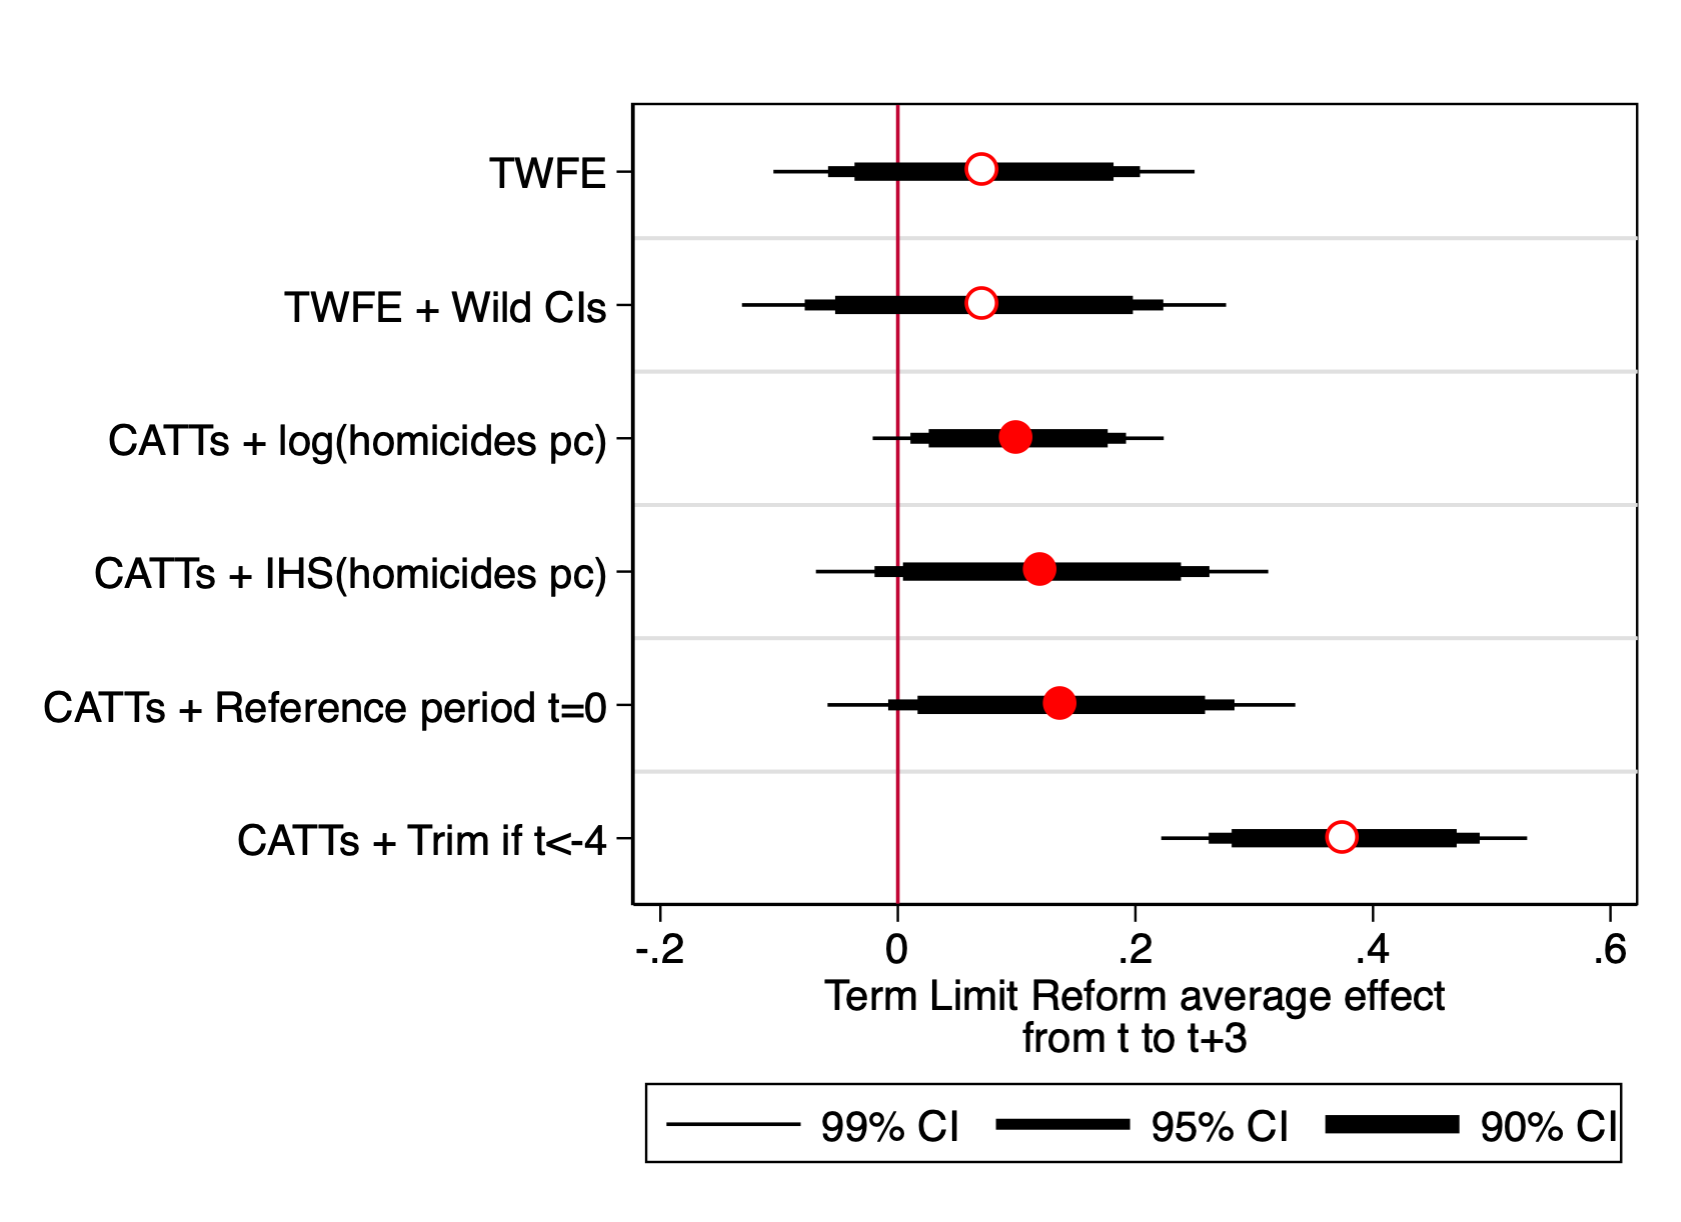
\includegraphics[width=0.9\textwidth]{Figures/average_effects_homicides.png}
       \captionsetup{justification=centering}
       
 \textbf{Note:} Figure \ref{fig:robustness_violence} shows the average treatment effect from t to t+3 across multiple specifications. This average effect was estimated using the IW estimators following \citet{abraham_sun_2020} for each lead and lag relative to the first year a municipality implemented reelection. Red points show that parallel trends hold, while hollow ones imply pretrends. 
\end{figure}      

\begin{figure}[H] 
\centering
 \caption{Effect of Term Limit Reform on Violence, propensity score matching on pretreatment covariates}
 \label{fig:matching_violence}
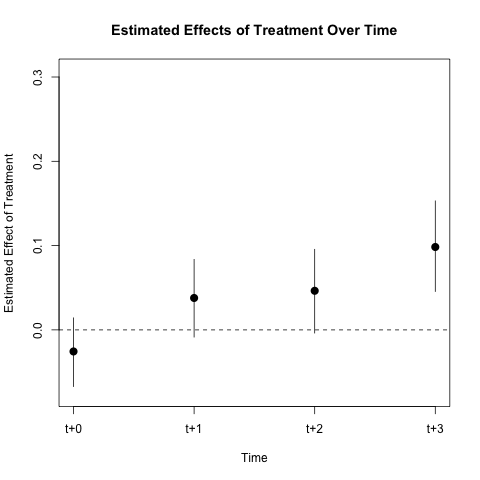
\includegraphics[width=0.75\textwidth]{Figures/panelmatch_logdefuncionespc.png}
       \captionsetup{justification=centering}
    
        
 \textbf{Note:} Figure \ref{fig:matching_violence} produced by propensity score matching that adjust for the treatment and covariate histories during the 5 year periods prior to the treatment. I report 95\% bootstrap confidence intervals clustered at the state level. Covariates include those used to generate Figure \ref{fig:event_study_agreements}. 
 
\end{figure}   
           
    
    
 \clearpage   
 
 %%%% NO ANTICIPATORY ASSUMPTION   
\section{Validating the no-anticipatory assumption \label{appendix:CDLZ}}

\renewcommand{\thetable}{C-\arabic{table}}
\setcounter{table}{0}
 \renewcommand{\thefigure}{C-\arabic{figure}}
\setcounter{figure}{0}
    
         
One way to address the no-anticipatory behavior is to assume that it can only occur in a fixed window prior to the electoral reform, say of one year, especially since the reform was announced in early 2013. However, for states that implemented reelection later this fixed window assumption would not suffice. In other words, only those early adopters of the reform would show unbiased estimates. Late adopters, however, would anticipate the term limit removal an act accordingly biasing the results upwardly.  
 
Another way to assess the no-anticipatory behavior from incumbents in this setting is test whether early vs late adopters differed in their estimated effects. Appendix Figure \ref{fig:CDLZ_agreements} presents \citet{cengiz_etal_2019} ``event-by-event analysis" that estimates treatment effects for each treated Mexican state (28 states) in the sample. States color differs if they are early (2015, red color) or late adopters (2016-2018, blue color). Specifically, I create state-event specific panel datasets and estimate state-specific estimates using separate regressions for each state. Each state dataset contains the treated state and all other states that never received treatment or received treatment after the sample window of $t+1$. For each state I estimate the following DiD regression: 
   
\begin{equation}
y_{mt}=\mu_m	 + \mu_t + \gamma Reform_{mt} + \epsilon_{mt}
\end{equation}

where $Reform_{mt}$ is an indicator variable that takes the value of 1 if the state implemented reelection. If there was evidence of strong incumbent anticipatory behavior, conditional on state covariates such as governor winning margin and alignment with Federal Executive, we would expect strong color clustering across similar estimated effects. In other words, if there is an endogenous response by states to implement the electoral reform, we would see that the positive (or negative) treatment effect would be only by those that implemented reelection earlier or later (events with the same color would be clustered). However, as seen in Appendix Figure \ref{fig:CDLZ_agreements}, this is not the case: there is wide variation in estimated coefficients across early (red) and late (blue) adopters of the reform, conditional and unconditional on state covariates. One would be concerned of the five blue states clustered in the positive end. However, if there was anticipation in these states they would only represent a downward bias of the main results found on the paper.  

\begin{figure}[h]
\centering
\caption{``Event-by-event analysis'' following \citet{cengiz_etal_2019}\\ -95\% confidence intervals-} 
\label{fig:CDLZ_agreements}
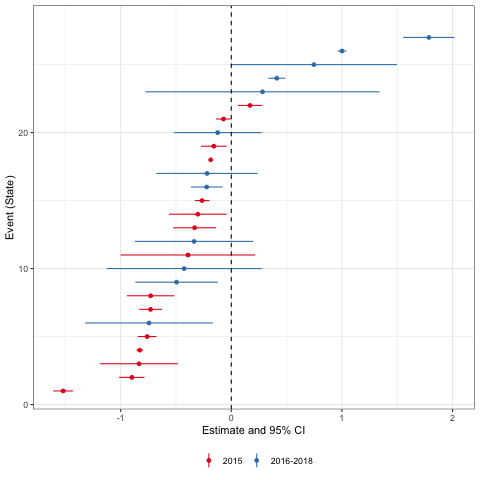
\includegraphics[width=0.5\textwidth]{Figures/CDLZ_cov_acuerdo.png}
       \captionsetup{justification=centering}
       \\
 {\textbf Note:} Estimate separate treatment effects for each event, i.e. each Mexican state in the sample. Each event dataset contains the treated state and all other states that never received treatment or received treatment after the sample window ($t+1$).   
\end{figure}     
   
For robustness, Appendix Figure \ref{fig:stacked_wcontrols_agreements} presents the ``stacked dataset analysis" from \citet{cengiz_etal_2019}. I take each of the ``event-by-event'' datasets from the Appendix Figure \ref{fig:CDLZ_agreements}, stack estimates by cohort and estimate one set of lead and lag variables not using prior treated units as controls. Appendix Figure \ref{fig:stacked_wcontrols_agreements} shows that conditional on state-level covariates, there is strong evidence of parallel trends as well as negative effect of reelection on delegation, but noisy.
       
    
\begin{figure}[H]
\centering
\caption{``Stacked dataset analysis'' following \citet{cengiz_etal_2019}\\ -95\% confidence intervals-} 
\label{fig:stacked_wcontrols_agreements}

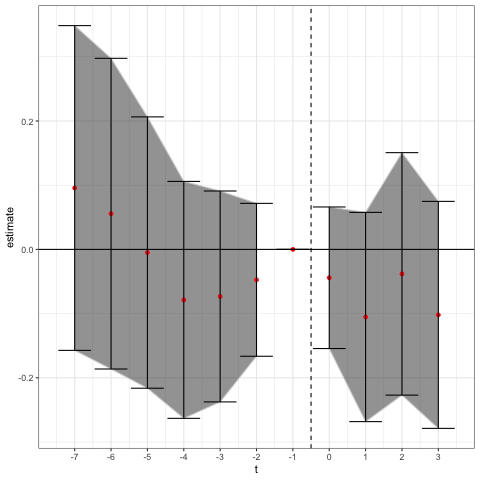
\includegraphics[width=0.5\textwidth]{Figures/stacked_dataset_wcontrols_acuerdo.png}
       \captionsetup{justification=centering}
       \\
 {\textbf Note: Utilize estimated coefficients from Figure \ref{fig:CDLZ_agreements} and stack them in relative time, and estimate lead and lag variables to treatment following the event-by-event analysis setup, i.e. without treatment containment from using prior treated units of controls. Analysis done stacking at the cohort level, and adding municipality and year fixed effects, and clustered standard errors at the state level.}     
\end{figure}   


\clearpage
   
%%%%%%%%%%%%%%%%%%%%%%%%%%%%%%%%% 

  
\end{document}
